%% The Diodic Search Architecture
%%
%% Template: a clean single-column 11pt article in the classic preprint
%% school (NeurIPS / arXiv look): one column, 1in margins, Times-like Newpx
%% text and math, a centred title block, an unboxed abstract, bold
%% size-contrast section headings. The IEEEtran `journal+onecolumn`
%% choice would buy proof-friendly single-column measure at the cost of an
%% institutional masthead this preprint does not need; every theorem,
%% table, figure and listing dependency is asked for explicitly below, so
%% nothing about the body is tied to a venue class.
\documentclass[11pt,letterpaper]{article}

\usepackage[margin=1in]{geometry}
\usepackage[T1]{fontenc}
\usepackage{amsmath,amsthm}
\usepackage{newpxtext}
\usepackage{newpxmath}
\usepackage{booktabs,array,tabularx}
\usepackage{graphicx}
\usepackage{xcolor}
\usepackage{microtype}
\usepackage{enumitem}
\usepackage{xurl}
\usepackage{tikz}
\usetikzlibrary{arrows.meta,positioning,calc}
\usepackage{listings}
\usepackage{titlesec}
\usepackage{hyperref}

%% One colour for both figures and code rules, so they read as a set.
\definecolor{rgxblue}{HTML}{1F4E79}
\hypersetup{colorlinks=true,linkcolor=rgxblue,citecolor=rgxblue,urlcolor=rgxblue,
  pdftitle={The Diodic Search Architecture: Regex Search without
    Per-File Metadata Cost},
  pdfauthor={Dan Alec Yamaguchi}}

%% cleveref refuses to load before hyperref, so it goes last.
\usepackage{cleveref}

\crefname{lstlisting}{Listing}{Listings}

%% Section headings: the classic preprint look --- bold, size contrast,
%% light spacing, no rules, no boxes.
\titleformat{\section}{\large\bfseries}{\thesection}{0.75em}{}
\titleformat{\subsection}{\normalsize\bfseries}{\thesubsection}{0.75em}{}
\titleformat{\subsubsection}{\normalsize\itshape}{\thesubsubsection}{0.75em}{}
\titlespacing*{\section}{0pt}{2.2ex plus .8ex minus .2ex}{1.2ex plus .2ex}
\titlespacing*{\subsection}{0pt}{1.8ex plus .6ex minus .2ex}{0.9ex plus .2ex}
\titlespacing*{\subsubsection}{0pt}{1.5ex plus .5ex minus .2ex}{0.7ex plus .2ex}

\lstdefinestyle{rust}{
  basicstyle=\ttfamily\scriptsize,
  keywordstyle=\bfseries\color{rgxblue},
  commentstyle=\itshape\color{gray!70!black},
  showstringspaces=false,
  breaklines=true,
  frame=leftline,
  framerule=0.6pt,
  rulecolor=\color{rgxblue!45!black},
  xleftmargin=1.6ex,
  numbers=left,
  numbersep=4pt,
  numberstyle=\tiny\color{gray},
  aboveskip=8pt,
  belowskip=4pt,
}
\lstdefinelanguage{Rust}{
  morekeywords={pub,fn,let,mut,unsafe,for,in,as,struct,impl,self,match,
                if,else,loop,while,return,true,false,where,use,crate,mod},
  morekeywords={i8,i16,i32,i64,isize,u8,u16,u32,u64,usize,f32,f64,bool},
  sensitive=true,
  morecomment=[l]{//},
  morestring=[b]",
}
\lstset{style=rust}

%% The theorem environments the proofs are written against. amsthm's plain
%% style, which is what the famous papers use: italic body, upright label.
%% Each environment numbers itself. Sharing one counter through [theorem] reads
%% tidier and is a common habit, but cleveref takes the reference type from the
%% counter name, so \Cref{rem:littl} printed "Theorem 3" for a remark -- the
%% heading said Remark and every reference to it said Theorem.
\newtheorem{theorem}{Theorem}
\newtheorem{lemma}{Lemma}
\newtheorem{proposition}{Proposition}
\newtheorem{definition}{Definition}
\newtheorem{corollary}{Corollary}
\newtheorem{remark}{Remark}

%% Let TeX buy a little slack rather than overrunning the measure.
\setlength{\emergencystretch}{1.2em}

%% This paper is table-heavy and two of its tables are tall. With the
%% default float fractions a tall table cannot share a page with text and
%% one deferred float queues every float behind it, so all of them flush at
%% the end of the document. Generous fractions keep each table near its
%% text, which is where a reader needs it.
\renewcommand{\topfraction}{0.92}
\renewcommand{\bottomfraction}{0.8}
\renewcommand{\textfraction}{0.05}
\renewcommand{\floatpagefraction}{0.6}
\setcounter{topnumber}{3}
\setcounter{totalnumber}{4}

\begin{document}

\begin{center}
{\LARGE\bfseries The Diodic Search Architecture:\\[0.35em]
Regex Search without Per-File Metadata Cost}\\[1.3em]
{\large Dan~Alec~Yamaguchi}\\[0.45em]
{\scshape Independent Researcher}\\[0.25em]
{\small\texttt{danalec@gmail.com}\quad\textbullet\quad
ORCID~\href{https://orcid.org/0009-0002-9725-7779}{0009-0002-9725-7779}}\\[0.7em]
{\small Preprint --- not peer reviewed; comments welcome.
Manuscript dated \today.}\\[0.2em]
{\small Hosted on Zenodo as a 2026 preprint.}\\[0.2em]
{\small DOI~\href{https://doi.org/10.5281/zenodo.23453407}{10.5281/zenodo.23453407}}\\[0.2em]
{\small Code:~\href{https://github.com/danalec/rgx}{\texttt{github.com/danalec/rgx}}}
\end{center}

\vspace{0.8em}

\begin{abstract}
\noindent
We present a prepared-corpus regex search system that reduces
repeated-query latency by amortizing per-file filesystem metadata costs
into a one-time packing and indexing phase. A SIMD candidate filter
reduces exact-match work but introduces no false negatives. On stable
corpora with many small files the system achieves substantial end-to-end
speedups --- 2.79--3.38$\times$ over ripgrep~15 on a fixed 20{,}000-file
corpus and 6.66--12.41$\times$ on a live 95{,}942-file, 1.94~GB registry
across the patterns whose result sets coincide, breaking even at
$Q^{*}\approx 24$ queries --- and the advantage
diminishes for one-shot searches or frequently changing corpora. An
in-process timer reports a phantom 53.9\% win for a leaked unmap that the
external wall clock refuses, and every end-to-end performance claim in this
paper rests on external wall-clock measurements; the in-process timings are
reported separately as diagnostics, for the segments they explain and nothing
more. Count parity holds on every comparison reported here except the two
live-registry patterns marked $\dagger$ in \Cref{tab:cargo}, where the store returned
a strict subset of the direct engine's answer; no ratio is claimed for them,
and both endpoints of the registry range come from coinciding patterns. Even
there the store arm of that snapshot did not extract container text, so the
range is a property of that historical configuration --- the missing work could
have lowered the store's cost without changing its answer --- and this paper
reports no full-pipeline registry measurement. The
Tesla valve serves as an
architectural inspiration for asymmetric cost, not as a physical model or
performance explanation.
\end{abstract}

\vspace{0.6em}
\noindent\textbf{Keywords.} search, regular expressions, SIMD, storage
architecture, filesystem metadata, amortisation, AVX2, bitmask, multiscale
modelling, queueing, Bloom filters.
\vspace{0.8em}

\section{Introduction}
\label{sec:intro}

\subsection{The filesystem metadata ceiling}
State-of-the-art grep implementations, exemplified by ripgrep
\cite{ripgrep}, reach multi-gigabyte-per-second throughput on a single large
contiguous file by pairing vectorised literal search \cite{qiu2021teddy,
hyperscan} with automata engines \cite{regexautomata}. When searching a
codebase $\mathcal{C}=\{f_1,\dots,f_N\}$ of $N$ small files with mean length
$\bar{L}$, total latency decomposes as
\begin{equation}
\label{eq:direct}
T_{\text{direct}} = T_{\text{discovery}} + T_{\text{metadata}}
  + T_{\text{read}} + T_{\text{match}} + T_{\text{output}} ,
\end{equation}
where $T_{\text{discovery}}$ is recursive directory enumeration with
\texttt{.gitignore} evaluation, $T_{\text{metadata}}$ is synchronous
per-file kernel transition (path resolution, \texttt{fstat} or
\path{GetFileInformationByHandle}, \texttt{open}/\texttt{close}),
$T_{\text{read}}$ is non-contiguous small I/O, $T_{\text{match}}$ is in-memory
matching, and $T_{\text{output}}$ is serialisation and terminal
synchronisation. File sizes in software repositories are heavy-tailed: in the
93{,}234-file Cargo registry corpus of \Cref{tab:nine} the
median length is $4.4$~KiB. In this regime \eqref{eq:direct} is dominated by
its first two terms, and the regex core idles while the CPU stalls on kernel
locks and directory table lookups.

Two structural facts make the ceiling a systems problem rather than a
pattern-matching problem. First, the first three terms of
\eqref{eq:direct} are \emph{per-file} while the last two are
\emph{per-byte}: whatever the engine does, a walk over $N$ files pays
$\Omega(N)$ metadata transactions before a single match decision is made.
Second, the per-file terms do not vectorise --- they are synchronous kernel
transitions with a transaction quantum of one file. The result is a
\emph{scale separation}: on a 246~MB single file the engine is the whole
cost and the in-house engine can lead ripgrep substantially on some
pattern shapes (up to $+114\%$ on the primary host of \Cref{sec:eval}, and
$+40\%$ on a second host), while on a 20{,}000-file tree of the same total
bytes the same nine shapes collapse to parity or single-digit separation,
because the walk owns the budget. The single-file lead is
\emph{host- and shape-dependent}: the same corpus on a second machine
inverts the sign on six of the nine shapes (\Cref{sec:eval:cross}), so the
portable claim is the scale separation itself, not a particular matcher
margin. The engineering question is therefore not how to make the matcher
faster but how to change which term of \eqref{eq:direct} the query pays.

\subsection{Candidate explosion in the scalar confirmation path}
At the scanning layer, matchers identify candidates by looking for rare
literals or literal pairs. For a pattern whose prefix literal is
high-frequency and whose secondary constraint is selective --- \texttt{e[0-9]},
\texttt{foo.*bar} --- the forward scan produces far more candidate offsets
than there are matches. Each surviving offset is confirmed by a scalar
routine, so the number of scalar entries, not the number of matches, is what
the branch predictor and the dispatch path have to absorb. The ratio of
admitted candidates to naive prefix candidates is the quantity a filter
should minimise, or equivalently the ratio of naive to admitted is what it
should maximise; \Cref{sec:dio} names it, measures it, and
\Cref{sec:foundations} proves that reducing it cannot lose a match.

\subsection{Contribution}
This paper contributes: (i) a two-term multiscale cost model of search
latency, $T=\sigma N+B/\beta$, and a storage tier that removes the
$\mathcal{O}(N)$ metadata term from the query path by paying it once at
ingestion (\Cref{sec:theory,sec:storage}), together with a proof that
prepared in-slice search is semantically identical to isolated per-file
search (\Cref{thm:equivalence}); (ii) a formal amortisation threshold
$Q^{*}$, drawn as a phase boundary in the query-per-mutation plane, beyond
which the prepared store is strictly cheaper (\Cref{thm:breakeven} and
\Cref{sec:regimes}), together with the observation that this boundary is a
statement about workload shape rather than about regex search --- it maps
onto dependency-tree search, log partitions, reference-database lookup and
e-discovery alike (\Cref{sec:uses}); (iii) a compilation, at compile time,
of a pattern's necessary
byte conditions into a rectangle cover of the nibble grid --- evaluated as
a branchless OR of ANDs in vector registers, with a proof of zero false
negatives and an abstract-interpretation reading of why
(\Cref{sec:foundations:abs,sec:micro}); (iv) an empirical audit, in the
measurement-theory sense, of the naive physical intuition behind
memory-mapped I/O, whose teardown accounting alone reports a phantom
53.9\% win for the leaked unmap --- an accounting result, not a property of
mapping --- that no wall clock confirms (\Cref{sec:mmap}); and (v) a
cross-host replication
(\Cref{sec:eval:cross}) that separates what the architecture guarantees
from what a particular machine happens to measure: the pack store's
advantage and the buffered-over-mmap direction transfer across OS and CPU
class, the headline multipliers and the matcher margins do not. A sixth
finding is a negative one about reporting: a column mislabel in the n-gram
harness output manufactured a 512-bit ``inversion'' against the Bloom
model that the measurements never contained, and
\Cref{sec:ngram:inversion} records the error because a mechanism that
explains a non-event is worse than no mechanism. Where a magnitude still
depends on regime --- a streaming advantage over memory mapping that
separates at $-43.5\%$ to $-67.3\%$ on scan-bound count cells of the 93k
store, narrows to $-9.8\%$ to $-11.2\%$ on full-output cells, and overlaps
at the 20k scale --- we state the cell with the number and bound the claim
(\Cref{sec:mmap,sec:limits}).

\subsection{Claims, and what would falsify each one}
\label{sec:claims}
The thesis is falsifiable in one sentence: \emph{for a corpus of $N$ small
files whose prepared query path costs $T_{\text{tv}}<T_{\text{direct}}$ per
query at exact result parity, consolidating the corpus into contiguous packs
at ingestion reduces the cumulative build-plus-query cost once the number of
queries served per invalidation cycle exceeds $Q^{*}$ of \eqref{eq:qstar};
within the two-term model, eliminating only the metadata term bounds the
idealized per-query speedup at $1+\rho$, where $\rho=\sigma N/(B/\beta)$ is
that corpus's metadata-to-scan ratio (\Cref{prop:separation})}. Everything else the paper says is evidence for
that sentence, a mechanism it needs, or an analogy that predicts nothing.
Concretely the split is three-way: three \emph{proved} claims (in-slice
search over the prepared store is result-identical to isolated per-file
search, the compiled mask never removes a true match start, and for
fixed-width byte-class patterns and their pointwise codepoint lifts matching
agrees offset for offset on a pure-ASCII window --- the
window rule of Appendix~\ref{app:window}, machine-checked in Lean~4), one
\emph{empirical} class (gated end-to-end wall clock on stable corpora of
many small files, where the prepared arm wins past $Q^{*}$), and one
\emph{analogy} (the valvular conduit motivated the idea of asymmetric
cost; it neither explains the gain nor predicts performance).
The failure mode of this class of paper is a performance number that is
really an analogy, or an analogy quoted as a prediction, so
\Cref{tab:claims} sorts every claim by kind and names what would falsify
it. ``Proved'' means a theorem under stated preconditions;
``measured'' means a number with a host and a date attached;
``analogy'' carries no empirical content; and the last row is on the
table precisely so that it cannot be silently assumed.

\begin{table}[htbp]
\centering
\footnotesize
\caption{The claims of \Cref{sec:claims}, by kind and by falsifier. A claim
not on this table is not made. Performance rows are falsified only by a
gated run --- one whose counts agree --- since a faster time on a smaller
result refutes nothing.}
\label{tab:claims}
\begin{tabular}{@{}>{\raggedright\arraybackslash}p{0.28\linewidth}>{\raggedright\arraybackslash}p{0.14\linewidth}>{\raggedright\arraybackslash}p{0.17\linewidth}>{\raggedright\arraybackslash}p{0.29\linewidth}@{}}
\toprule
\textbf{Claim} & \textbf{Kind} & \textbf{Evidence class} & \textbf{What would falsify it} \\
\midrule
in-slice search over a prepared store is result-identical to isolated per-file search
  & correctness & proved (\Cref{thm:equivalence}) & one match, offset, line, column or context line that differs between the two paths \\
the compiled mask never removes a true match start
  & correctness & proved (\Cref{thm:fnr}) & a match at an offset the mask does not admit \\
for fixed-width byte-class patterns, matching agrees with its codepoint lift on a pure-ASCII window
  & correctness & proved, machine-checked (\Cref{thm:window}) & a fixed-width byte-class pattern and a pure-ASCII window whose match verdicts differ between the two semantics \\
packing removes the syscall-class $\mathcal{O}(N)$ term from the query path
  & performance & measured (\Cref{sec:eval}) & a gated run on a many-small-files corpus where prepared latency grows with $N$ at fixed $B$ \\
the per-file paths pay a page-cache penalty of $30$--$38\%$ of their warm latency
  & performance & measured twice (\Cref{sec:eval:cold}) & a cold/warm pair on which the per-file arms show no penalty \\
n-gram signatures prune files before any slice is borrowed
  & performance & measured standalone (\Cref{tab:ngram}) & a pruned file the query would have printed \\
the mask reduces the candidate stream where the constraint is selective
  & performance & measured, one corpus (\Cref{tab:dio}) & a selective constraint quenching no more than a dense one \\
the combination lowers end-to-end latency past $Q^{*}$
  & performance & measured, host-bound (\Cref{tab:small,tab:cargo,tab:linux}) & a gated paired run where the store loses to both direct arms at $Q>Q^{*}$ \\
the phase boundary carries to other workload shapes
  & generality & argued, not measured (\Cref{sec:uses}) & a domain meeting the three conditions there where preparation loses \\
the amortisation boundary governs name search at filesystem scale
  & generality & measured (\Cref{tab:names}) & a name workload where the indexed arm loses past its own break-even count \\
the valvular conduit picture organises the design; its residue is the calculus that finds the prefilter
  & explanatory & design method (\Cref{sec:calculus}) & a shipped prefilter component the calculus cannot derive, or a same-budget term set that suppresses less than the one it selects \\
the valvular conduit picture predicts or causes the speedup
  & --- & \emph{not claimed} & --- \\
\bottomrule
\end{tabular}
\end{table}

\section{A multiscale cost model of search latency}
\label{sec:theory}

\subsection{Background: where the picture comes from, and where it stops}
\label{sec:valve}
The system this paper measures is called \emph{diodic} for the shape of its
mechanism: one-way cost, scoped to a \emph{generation} of the corpus. A
mutation re-pays the build, so the asymmetry is amortisation between one
ingestion and many queries within a generation, not a law that survives
mutation.

\paragraph{The picture in one paragraph.}
Tesla's 1920 valvular conduit (US~Patent 1{,}329{,}559) \cite{tesla1920} is a
periodic sequence of asymmetric cavities: forward flow stays attached to a
streamlined channel and pays ordinary friction; reverse flow separates at a
blunt edge, recirculates, and re-enters the main channel at an adverse
angle, where its momentum is dissipated. A p--n junction is the same shape
in silicon --- a forward drop, a reverse leakage, and a breakdown voltage
past which the device conducts in the direction it is meant to block.
Both devices rectify by \emph{geometry}; neither seals. The compiled mask
of \Cref{sec:micro} is the third face of the same shape in bits: a
candidate stream enters, noise is discarded in place, and only admitted
candidates are forwarded. The diodicity
\begin{equation}
\label{eq:di}
Di = \frac{\Delta P_{\text{reverse}}}{\Delta P_{\text{forward}}}
\end{equation}
is the ratio of the two losses. A single element reaches single digits;
stages are chained to raise it; under enough back-pressure the device
still passes fluid the wrong way. It rectifies, it does not seal. Every
claim below inherits that limitation.

\paragraph{The correspondence, stated once.}
The architecture borrows two things from this picture and nothing else:
the \emph{asymmetry of work organisation} (high-friction terms pushed into
a one-off maintenance direction; the hot path kept streamlined) and, at
the register level, a genuine \emph{rectification} of a bidirectional
candidate stream (noise suppressed in place, matches forwarded). Where
the picture and the code disagree, the code is the claim. The detailed
correspondences between fluidic elements and computational elements, and
what each row would need to become a rigorous model rather than a
picture, are listed in \path{benchmark/analogy-grading.md} (a side-table
of the same rows that once lived here); the only correspondence the rest
of the paper relies on is the register tier, where the diode names a real
computation --- the discard-only filter of \Cref{sec:foundations:abs} ---
and the storage tier, where the design organises around the principle
without claiming that bytes flow.

\subsection{Demarcation: analogy versus inspiration}
\label{sec:demarcation}
We state the boundary explicitly, because conflating the two is the easiest
way to make this class of claim unfalsifiable.

\begin{itemize}[leftmargin=*,itemsep=1pt]
\item \textbf{Storage tier (\texttt{rgx-tv}) --- architectural inspiration.}
Loose files do not flow backwards through pipes. What the storage
architecture embodies is \emph{asymmetric work organisation}: the
high-friction terms of \eqref{eq:direct} are moved into an amortised
maintenance loop, and the high-frequency query path traverses a contiguous
pack with no per-file filesystem metadata calls. The fluid picture motivates the
\emph{shape} of the design; it makes no claim that bytes are fluid.
\item \textbf{Microarchitectural tier --- true functional analogy.} Inside
vector registers the mechanism is a real analogue: no branch instruction
(\texttt{cmp}/\texttt{jne}), no branch-predictor state, and no scalar state
transition occurs while candidates are being eliminated.
\Cref{sec:micro} states the mechanism precisely and \Cref{sec:limits}
states its limits.
\end{itemize}

\paragraph{The valve is not a model of this system, and predicts nothing
from it.}
No equation of motion in this paper computes a latency: the continuum
quantities of \Cref{sec:model} are a vocabulary for scale separation, and
the diodicity of the physical device does not enter any prediction. The
direction of explanation runs one way only --- the engineering is explained
\emph{to a reader} in the fluid picture, never derived from it --- and the
architecture's performance claims are falsifiable only against
\eqref{eq:twoterm} and the measurements of \Cref{sec:eval}, exactly as
\Cref{tab:claims} records. The analogy's residue is design discipline
(pay the friction once, in one direction; keep the other direction
streamlined) and vocabulary; where the picture and the code disagree, the
code is the claim. The residue is made operational in \Cref{sec:calculus}:
the discipline becomes a procedure, and the procedure's product is the
prefilter --- found, not described. The one place a formal object stands
in for the picture is the register tier, where ``rectification'' names a real computation:
the discard-only filter of \Cref{sec:foundations:abs}, which is defined
over candidate sets and not over fluids.

\subsection{The two-term transport model}
\label{sec:model}
Write the corpus as $N$ files totalling $B$ bytes, and let a query touch
every file (the worst case, and the honest one for a rare pattern). Direct
search has the scaling law
\begin{equation}
\label{eq:twoterm}
T_{\text{direct}}(N,B) = \sigma N + \frac{B}{\beta} + \varepsilon ,
\end{equation}
where $\sigma$ is the per-file metadata tax in
\eqref{eq:direct} ($T_{\text{discovery}}+T_{\text{metadata}}+T_{\text{read}}$
divided by $N$, dominated by the first two), $\beta$ is the effective scan
bandwidth once bytes are addressable, and $\varepsilon$ collects output.
Every measurement of $\sigma$ in this paper is a warm-cache number and so
an upper bound on the filesystem's share of the per-file cost;
\Cref{sec:eval:cold} splits the term against page-cache state and finds
the per-file paths paying $30$--$38\%$ of their warm latency going cold.
What that section does \emph{not} establish is that the prepared path is
better off: its own cold penalty moved by $50\times$ between two runs three
days apart, and the claim did not survive.
The two terms scale differently: $B/\beta$ counts bytes however they are
distributed across files (though its coefficient is not packaging-blind ---
$\beta_{\text{pack}}$ can differ from $\beta$, and \Cref{sec:mmap} measures
which the hardware prefers), while $\sigma N$ counts \emph{files}. A prepared store pays
$\sigma N$ once at ingestion and thereafter
\begin{equation}
\label{eq:twoterm-tv}
T_{\text{tv}}(N,B) = \sigma' N + \frac{B}{\beta_{\text{pack}}} + \varepsilon' ,
\end{equation}
with $\beta_{\text{pack}}\le\beta$ a possibly lower sequential bandwidth
(\Cref{sec:mmap} measures the trade) and $\sigma'$ the per-file
\emph{arithmetic} residue of the query path --- a slice bound, a flag test,
a fresh line state --- with no kernel transition in it. The architecture's
claim is not that $\beta_{\text{pack}}>\beta$ --- it is usually not --- and
it is not that the $N$-dependence vanishes; it is that its coefficient
drops from a syscall-class constant $\sigma$ to an arithmetic-class
$\sigma'$ with no syscall in the term at all. Packing keeps the $N$ and
changes what multiplies it --- the equation is honest about that: the
$N$-dependence does not vanish, it stops being kernel work. The
residue $\sigma' N$ is small enough to sit under the floor of every timing
in \Cref{sec:eval}, so in practice \eqref{eq:twoterm-tv} reads as
$\sigma' N$ absorbed into $\varepsilon'$; a corpus with $N$ large enough
for $\sigma' N$ to surface at fixed $B$ would show prepared
latency still creeping with file count, and that experiment is not run
here (\Cref{sec:future}). Where the prose below says the store's query path has ``no $N$'',
the claim is ``no syscall-class $N$'' --- the distinction is the whole
content of \eqref{eq:twoterm-tv}.

\begin{proposition}[Scale separation of the metadata tax]
\label{prop:separation}
Let $\rho = \sigma N / (B/\beta)$ be the metadata-to-scan ratio of a
direct query (its metadata \emph{share} of the two-term total is
$\rho/(1+\rho)$).
When $\rho \gg 1$ (many small files), a matcher-only improvement and a
transport-only improvement are bounded by complementary terms of
\eqref{eq:twoterm}. Driving the match cost to zero while the metadata tax
stands still yields
\begin{equation}
\label{eq:smax}
S_{\max}^{\text{(match only)}} = \frac{\sigma N + B/\beta}{\sigma N}
  = 1 + \frac{B}{\beta\,\sigma N} = 1 + \rho^{-1} ,
\end{equation}
and conversely eliminating only the metadata term leaves at most
$1 + \rho$. As $\rho \to \infty$ the first bound tends to $1$ and the
second diverges: on a many-small-files corpus, no amount of matcher work
can substitute for transport work, and the two tiers are complements
rather than competitors.
\end{proposition}

\begin{proof}
Immediate from \eqref{eq:twoterm} with one term driven to zero at a time.
\end{proof}

\Cref{prop:separation} is the quantitative form of the opening
observation: the two ceilings are $1+\rho^{-1}$ and $1+\rho$, and $\rho$
is the only number that sets their height. This paper does not instrument
the split of a direct query between per-file work and byte work, so
$\rho$ is not a recorded constant of its corpora; the closest the
measurements come is the zero-match row of \Cref{tab:cargo}, where
transport over 1.94~GB costs 220~ms against 1{,}465~ms of direct search
on the same bytes --- a ratio of $6.7$, which under \eqref{eq:twoterm} is
$1+\rho$ for that comparison if the two arms' byte-scan terms are
comparable. That reading is an interpretation of one row and not a
measurement of the split; it puts the matcher ceiling near $1.2\times$
and the transport ceiling near $6.7\times$. Both ceilings are
\emph{within-model}: they bound what changing one term can recover inside
one implementation's \eqref{eq:twoterm}, and a ratio between two
implementations --- ripgrep's per-file path against the store --- is not
bounded by them and may exceed the wider one, as the matching rows of
\Cref{tab:cargo} do. The two tiers are complements, not competitors, and
\Cref{lem:amdahl} below is this statement in its classical form.

\paragraph{The two-term law is an envelope, not a profiler.}
Equation \eqref{eq:twoterm} bounds how latency scales; it does not
decompose a query. When a query must be attributed rather than bounded,
the honest decomposition is
\begin{equation}
\label{eq:decomp}
T_{\text{query}} = T_{\text{setup}} + T_{\text{manifest}} + T_{\text{pack read}}
  + T_{\text{n-gram}} + T_{\text{mask}} + T_{\text{confirm}} + T_{\text{output}} ,
\end{equation}
and \Cref{tab:cost} names each term's unit, its isolating measurement, and
what bounds it. Two terms carry no isolated measurement in this paper and
sit under $\varepsilon'$ in every timing; the others have a named way to be
measured on its own. The terms are additive only in the accounting sense:
they overlap in a parallel run, which is why the paper's claims come from
paired end-to-end timings and from the count gate, never from a sum of
stage timers --- the stage-timer trap of \Cref{sec:mmap} is exactly the
failure of attributing an overlapped pipeline to its stages.

\begin{table}[htbp]
\centering
\footnotesize
\caption{The decomposition of \eqref{eq:decomp}, and how each term could be
measured in isolation. ``---'' marks the terms no experiment in this paper
isolates; they are absorbed in $\varepsilon'$ of \eqref{eq:twoterm-tv}.}
\label{tab:cost}
\begin{tabular}{@{}llp{0.36\linewidth}l@{}}
\toprule
\textbf{Term} & \textbf{Unit} & \textbf{Isolating measurement} & \textbf{Bound by} \\
\midrule
$T_{\text{setup}}$ & ms & --- (process start, pattern compile) & CPU \\
$T_{\text{manifest}}$ & ms & --- (manifest parse; $O(N)$ records) & CPU, memory \\
$T_{\text{pack read}}$ & ms & the zero-match probe of \Cref{tab:cargo} minus setup & I/O (memory when warm) \\
$T_{\text{n-gram}}$ & ns/file & the per-file filter latency of \Cref{tab:ngram} $\times\,N$ --- standalone; \Cref{sec:ablations} runs it end to end and finds no wall-clock gain above the floor & CPU (L1-resident) \\
$T_{\text{mask}}$ & GB/s & the scalar reference of \Cref{tab:dio}, or the vector loop on the same bytes & CPU (registers) \\
$T_{\text{confirm}}$ & ns/candidate & the same run with and without the mask on a dense shape & CPU \\
$T_{\text{output}}$ & ms & the \texttt{-c} arm against the full-output arm of \Cref{tab:nine} & CPU, terminal I/O \\
\bottomrule
\end{tabular}
\end{table}

\subsection{Continuum limit and head loss: where the analogy stops}
The Knudsen and Darcy--Weisbach analogy is bookkeeping for scale separation
here, not a predictor. The limiter's Knudsen ratio records whether the pack
window amortises at the scale at which it is evaluated; it does not predict
what the limiter does, which \Cref{sec:model} derives from the per-file term
$\sigma N$ and the two-term law instead. The Darcy--Weisbach minor-loss
coefficient is counted in syscalls and not measured in pressure, and no number
in this paper is derived from either analogy. Every prediction of
\Cref{sec:predictions} follows from \Cref{sec:model} alone.

\subsection{Queue dynamics, and the boundary of the picture}
\label{sec:queue-stub}
The picture supplies vocabulary (\emph{throughput}, \emph{backpressure},
\emph{queue}) but no equation. Task queues carry no momentum equation; the
worker pool is a closed queueing network whose throughput $X\le K/D$ is
set by Little's law and the I/O station's ceiling
$X\le\beta_{\text{pack}}/L_{\text{pack}}$. The pool realises backpressure
as a bounded channel whose send blocks, never as a continuum PDE. The
exclusion of Navier--Stokes and the LWR fluid limit on this object is not
a prohibition of physics --- it is a statement about the dynamics the
object has.

\begin{remark}[Navier--Stokes exclusion on data queues]
\label{rem:nse}
A sequence of work items has no shear stress and no pressure, so the force
law that makes Navier--Stokes predictive does not exist on the object. What a
task queue does have is a service-time distribution and an occupancy count,
which is the vocabulary the bound of \Cref{rem:littl} is written in. Any
continuum equation needing a momentum or a pressure gradient has no argument to
apply here, and the LWR fluid limit of \cite{lwr1955,richards1956} is excluded
for the same reason. This is a statement about the dynamics the object has, not
a prohibition of physics.
\end{remark}

\begin{remark}[Worker pool as a closed network]
\label{rem:littl}
Little's law \cite{little1961} bounds the pool at throughput $X\le K/D$ with
$D=\mathbb{E}[S_{\text{claim}}]+\mathbb{E}[S_{\text{scan}}]$. The results that
sharpen Little's law for large closed networks --- Kingman's heavy-traffic
limit \cite{kingman1962}, Halfin--Whitt \cite{halfinwhitt1981}, Dai's fluid
limit \cite{dai1995} and Le Boudec's network calculus \cite{leboudec2001} ---
are named rather than applied, because $K$ is a small integer fixed by the
harness and not a growing population, so none of the scaling regimes they
describe is entered here. The bound that does bind is the I/O station's
ceiling $X\le\beta_{\text{pack}}/L_{\text{pack}}$: with enough workers the
network saturates the I/O station, and adding workers beyond that point
changes nothing.
\end{remark}

The end-to-end latency predictions of \Cref{sec:predictions} are made and
tested without invoking this remark pair.

\subsection{Where each quantity lands in the code}
The model above is not decoration on an implementation that owes it nothing.
The list below names each \emph{quantity} and says which part of the system
it is and where it is measured.
\begin{itemize}[leftmargin=*,itemsep=1pt]
\item $\sigma N$ in \eqref{eq:twoterm} is the metadata tax: the walk, the
  \texttt{stat}, the \texttt{open} and the close that precede every byte of
  a small file. \Cref{sec:storage} removes it at ingestion; the zero-match
  row of \Cref{sec:eval:cargo} is the closest the measurements come to
  isolating it.
\item $B/\beta$ and $B/\beta_{\text{pack}}$ in \eqref{eq:twoterm-tv} are
  the two transport legs --- many small random reads against a few large
  sequential ones --- and \Cref{sec:mmap} measures which the hardware
  actually prefers.
\item The pack unit is the syscalls-killed barrier: 16~MiB of contiguous bytes
  against 64-byte transaction lines, which is the same statement as saying the
  traversal no longer stops at file boundaries.
\item The per-file syscall barrier count is $\approx 280{,}000$ on the live
  registry, reduced by \Cref{sec:storage} to 117 reads --- the
  \emph{minor-loss} term of the picture in the book's vocabulary, with no
  $K_L^{(k)}$ measured.
\item $Di$ in \eqref{eq:di} is not a metaphor at the register tier; it is
  the quench ratio of \Cref{tab:dio}, candidates eliminated per candidate
  admitted, and \Cref{sec:micro} compiles the constraints that set it.
\item The worker pool is a closed queueing network whose throughput stops
  rising when the I/O station saturates; the thread-count row of
  \Cref{tab:nine} is the empirical handle.
\end{itemize}
A reader who wants only the engineering may skip the background subsection
and lose no result; a reader who wants to check the engineering against the
model will find every term above in the section named beside it.

\paragraph{The picture's predictions.}
The fluid picture produces none of the predictions below; what it supplies
is a vocabulary (\emph{boundary, regime, rectification, throughput}) and a
discipline (pay the friction in one direction, keep the other streamlined).
The predictions themselves come from the two-term law, the scale-separation
bound, and the break-even theorem. The next section states them, pairs
each one with the measurement that tests it, and names which predictions
the measurements separate, which they cannot, and which are unchanged
inside the harness's $\pm 3$\% paired-run floor.

\section{Cost-model predictions vs measurements}
\label{sec:predictions}

Every quantitative claim of \Cref{sec:theory} is testable against the
measurements of \Cref{sec:eval}, and every measurement attaches to one of
them. \Cref{tab:predictions} pairs each prediction with the protocol that
tests it and the verdict; the rule is the same one \Cref{sec:eval} uses
throughout --- count parity, paired arms, a minimum of seven rounds, and a
verdict that may refuse rather than coerce. ``\emph{Separated}'' means the
two arms' \([\text{min}\,..\,\text{max}]\) ranges do not overlap;
``\emph{overlap}'' means the median direction holds but the spread does
not separate the two arms; ``\emph{unchanged}'' means the two arms are
within the harness's $\pm 3$\% paired-run floor and the prediction is not
tested by the row.

\begin{table}[htbp]
\centering
\footnotesize
\caption{Cost-model predictions, mapped to the measurement that tests each
one and the verdict on its host(s). $\rho = \sigma N/(B/\beta)$ is the
metadata-to-scan ratio of \Cref{prop:separation}; $Q^{*}$ is the
break-even of \Cref{thm:breakeven}. Hosts: W = Windows 7950X3D, L = Linux
Ryzen~7~255. The inter-quartile column reports the
$[Q_1,Q_3]$ of the \emph{ratio} across rounds; $[Q_1,Q_3]$ is what the
harness records and what is comparable across hosts. Each verdict cell names its
host and the transcript behind it: the fixed-tree aggregates come from
\texttt{benchmark/status.md} (W) and
\texttt{benchmark/status-linux-ryzen7-255.md} (L), the registry aggregate from
\texttt{benchmark/tv-transcript.md}, on the snapshots those files date. The
estimator here is the median and the $[Q_1,Q_3]$ of the \emph{per-round ratio},
which is not the ratio of per-pattern minima printed in
\Cref{tab:small,tab:cargo,tab:linux}: a minimum over seven paired rounds is an
optimistic order statistic and a median is a central one, so the two estimators
disagree by construction and neither corrects the other.}
\label{tab:predictions}
%% The four widths sum to 0.92 of the measure and the inter-column gaps run
%% at 3pt, so the table sits ~19pt inside the text block instead of 3.12pt
%% outside it. Ragged-right cells are the fix, not a preference: justified
%% prose in a column this narrow can only reach the width by stretching the
%% few words left around an unbreakable $[a,b]$ IQR, which is what the five
%% Underfull boxes were.
\setlength{\tabcolsep}{3pt}
\begin{tabular}{@{}>{\raggedright\arraybackslash}p{0.29\linewidth}>{\raggedright\arraybackslash}p{0.25\linewidth}>{\raggedright\arraybackslash}p{0.11\linewidth}>{\raggedright\arraybackslash}p{0.27\linewidth}@{}}
\toprule
\textbf{Prediction} & \textbf{Measurement} & \textbf{Hosts} & \textbf{Verdict (median $[Q_1,Q_3]$)} \\
\midrule
$\rho \gg 1$: store wins by removing $\sigma N$, not by speeding up the scan
  & end-to-end ratio on 20k small files vs. 95k files
  & W + L
  & \emph{separated}: fixed tree $2.4\times$ $[1.9,2.9]$ (W), $2.7\times$ $[2.1,3.4]$ (L); live registry $7.6\times$ $[4.9,11.2]$ (W), $9.1\times$ $[5.6,13.0]$ (W, second snapshot) \\
$\beta_{\text{pack}} \le \beta$: pack read is not faster, often slower
  & zero-match throughput floor
  & W
  & \emph{separated}: $8.8$~GB/s transport floor (1.94~GB / 220~ms); 5-round $[209,235]$~ms IQR \\
matcher ceiling $1 + \rho^{-1}$ rises with corpus size
  & diodicity ablation of \Cref{tab:ablation}
  & W + L
  & \emph{separated} on three shapes ($+109.6\%$, $+49.6\%$, $+23.5\%$); \emph{overlap} on $e[0-9]$ ($+7.6\%$); \emph{unchanged} on the five pure-literal shapes \\
$Q^{*} = T_{\text{build}}/(T_{\text{direct}}-T_{\text{tv}})$: tens of queries
  & $T_{\text{build}}$ vs. min-of-7 per-query savings
  & W + L
  & \emph{separated}: fixed tree $Q^{*}\!\approx\!24.1$ (W) and $21.3$ (L), IQR $[\pm 3.1,\pm 4.2]$; live registry $23.6$ and $17.3$ (both W, two snapshots) \\
$\mu\to 1$: store is overhead under mutation
  & mutation loop, two refresh ratios
  & W
  & \emph{separated}: $Q^{*}\!\approx\!9.6$ at $1\%$ mutation, $\approx 13.7$ at $10\%$ (5-round IQR $[\pm 1.1,\pm 1.4]$ queries) \\
\bottomrule
\end{tabular}
\end{table}

\paragraph{The overlap rows are not results.}
A prediction whose measurement overlaps the noise floor is named, not
hidden. The $e[0-9]$ ablation row separates at $+7.6\%$ in median but the
arms' \([\text{min}\,..\,\text{max}]\) ranges overlap
($[74.2\,..\,80.2]$ against $[77.6\,..\,85.9]$), and the harness refuses the
row as a result (\path{benchmark/findings.md}~\S 19). The five
pure-literal and line-window rows sit inside $\pm 3$\% and are reported
as \emph{unchanged}. The interpretation is direct: where the matcher is
asked to do very little work (no fallback anchor to lose) the diodicity
measurement is a placement metric, not a wall-clock predictor.

\paragraph{What the table does not predict.}
Cold-cache penalty is reported in \Cref{sec:eval:cold} as a measurement
of the present build, not as a prediction of the cost model. The model
bounds the warm path; the cold path is hardware, and a build that changes
the per-query manifest work also changes the cold penalty. The
measurements in \Cref{tab:cold} are valid for the build that produced
them and are not the basis of a portable claim.

\paragraph{CIs and sample budgets.}
The ratio column of \Cref{tab:predictions} reports the median and the
$[Q_1,Q_3]$ of the ratio across rounds, where each round is a paired
run. The minimum run budget is seven rounds; the cold-cache protocol
(\path{scripts/tv-cold.sh}) pays five samples per arm and quotes a
two-state fit
$T = T_{\text{warm base}} + \mathbb{1}_{\text{cold}} \cdot p$, with its
posterior spread, alongside the median difference $\Delta_{\text{med}}$.
Under five samples the fit's spread is $\pm 1.34$~ms, and is the
resolution available for any cold-cache number in this paper. The first
cold reading after a \texttt{drop\_caches} also faults in the binary's
text and the store manifest --- a MAD pass at
$3 \times 1.4826 \times \text{MAD}$ identifies exactly those samples and
nothing else, and the published penalty is the post-MAD fit. Where no
confidence interval is computed, ``$\pm 3$\%'' denotes the harness's
practical decision floor and not a statistical confidence interval;
interquartile ranges and model-based uncertainty estimates are reported
separately where available. Cross-session absolute drift moves by tens of
per cent (\Cref{sec:limits}), so a single ratio without its run date and
reference-arm placement is not compared across runs. The
\path{artifacts/INDEX.md} file lists which transcript and which corpus
digest back every numeric cell of the table.

\paragraph{Cross-host population.}
Two hosts are the population of every quoted cross-host claim (Windows
7950X3D + Linux Ryzen~7~255), and the rule of \Cref{sec:limits} holds:
ratios are properties of code \emph{and} machine. The architecture transfers
across OS and CPU class (the pack engine is faster than both direct paths
on every measured pattern, with exact count parity, on both hosts); the
matcher margin and the absolute timing do not. Two hosts do not bracket a
third: a host outside the pair could land on either side of them, or past
both, and nothing measured here decides it. What a second host does establish
is the shape of the disagreement --- which quantity moved and which held ---
and \Cref{sec:eval:cross} calls the rest the host-dependent part of the claim. The
$[Q_1,Q_3]$ columns in \Cref{tab:predictions} are the portable
observation: the \emph{range} holds across hosts even when the median
moves, which is what makes the prediction the same claim on both.

\paragraph{Predictions the model does \emph{not} make.}
The two-term law of \eqref{eq:twoterm} and the amortisation of
\eqref{eq:twoterm-tv} are scale laws: they bound how latency scales with
$N$ and $B$ and bound the gap between any two architectures that share
the same terms. They do not predict \emph{which} microarchitectural fill
is faster, do not predict the latency on a single file of one pattern
(the matcher dominates and the metadata tax is one term), and do not
predict the cache state of the box at the moment of the query.
\Cref{sec:future} lists the experiments that would either widen the
prediction set or sharpen its sample budget.

\section{Mathematical foundations}
\label{sec:foundations}

\subsection{Hermetic in-slice boundary isolation}
A common flaw in packfile search is string concatenation with a delimiter,
which produces cross-file match bleed, corrupted line numbering and broken
anchors.

\begin{definition}[Borrowed in-slice search]
Let $\mathcal{P}\in\Sigma^{*}$ be a contiguous binary pack of length
$\lvert\mathcal{P}\rvert$, and let $f$ index the byte interval
$[O_f, O_f+L_f)\subseteq[0,\lvert\mathcal{P}\rvert)$. The borrowed slice
$S_f$ is the exact subslice $S_f=\mathcal{P}[O_f\dots O_f+L_f-1]$,
searched without copying.
\end{definition}

\begin{theorem}[Semantic equivalence to isolated file search]
\label{thm:equivalence}
Let $R$ be a regular expression accepted by the parser of the matching
engine $\mathcal{M}$, let $f$ denote the bytes of a file \emph{as ingested}
into the store, and let $S_f$ be its borrowed in-slice representation. Then
the emitted match set $\mathcal{R}(S_f)$ is identical, in cardinality, byte
offsets, 1-based line numbering, column coordinates and context lines, to
an isolated execution of $\mathcal{M}$ over the same byte string $f$ stored
independently on disk.
\end{theorem}

\begin{proof}
Four invariants are orthogonal and jointly sufficient: each covers one part of
the equivalence, and it takes all four to cover the whole of it.
\begin{enumerate}[leftmargin=*,itemsep=1pt,topsep=2pt]
\item \textbf{Match extent isolation.} Automaton state transitions in
  $\mathcal{M}$ operate strictly on byte indices $j\in[0,L_f)$. The slice
  boundary is the haystack bound: the scan layer's vector loop admits only
  blocks whose full read window lies inside the slice and evaluates the
  remaining tail with the scalar predicate (\Cref{sec:micro}), so no byte
  outside $[O_f,O_f+L_f)$ enters any decision and every match span
  $[s_m,e_m)\subseteq[0,L_f)$. No match spans a file boundary.
\item \textbf{Anchor semantics.} The anchors
  \texttt{\textasciicircum}, \texttt{\textdollar},
  \texttt{\textbackslash b}, \texttt{\textbackslash A} and
  \texttt{\textbackslash z} are evaluated against the haystack bounds. Since
  the engine receives only $S_f$, index $0$ and index $L_f$ are the slice's
  own ends, and no adjacent file in $\mathcal{P}$ can influence the result.
\item \textbf{Strict 1-based line coordinates.} A fresh per-slice search
  state is constructed with $\text{line\_no}=1$ at offset $0$ of $S_f$, and
  each \texttt{\textbackslash n} in $S_f$ increments it. Line numbers
  therefore cannot accumulate across files in $\mathcal{P}$.
\item \textbf{Context clamping.} For a match on line $k$ with before-context
  $B$ and after-context $A$, the window is clamped to
  $[\max(1,k-B),\,\min(K_{\max},k+A)]$ where $K_{\max}$ is the line count of
  $S_f$. No line of a predecessor or successor file can enter the buffer.
\end{enumerate}
Hence $\mathcal{R}(S_f)\equiv\mathcal{R}(f_{\text{disk}})$.
\end{proof}

\paragraph{How the implementation realises this.}
\Cref{thm:equivalence} is a property of the slice, not of an object being
rebuilt per file. The matching engine and the compiled matcher are
constructed \emph{once per worker thread} and reused across every slice that
thread claims; what is re-instantiated per slice is the line-tracking state.
The worker therefore borrows $\mathcal{P}[\,O_f\dots O_f+L_f\,)$ and hands
it to a dispatch routine with the per-slice search state created inside that
call. The invariants are properties of \emph{any} engine meeting the
theorem's interface --- the shipped binary contains one such engine, the
in-house byte-mode matcher --- and the construction is exercised
end-to-end by the pack-store differential tests --- which compare the two
paths' answers in content, member paths included, and not merely in summed
counts ---
(\path{tests/cli.rs::a_pack_store_answers_what_the_direct_path_answers} and
\path{tests/cli.rs::an_incremental_update_keeps_the_pack_store_in_sync}),
by the boundary invariant enforced structurally at pack-build time
(\path{crates/rgx-core/src/tv/plan.rs::cut_units}, which refuses to cut a
match window across a file record), and by an equivalence fixture whose
patterns are chosen to match across a would-be pack boundary.

\paragraph{Preconditions, stated where they can be checked.}
The theorem is a statement about \emph{representations of the same byte
string}, and four preconditions delimit it. First, the pack holds corpus
bytes verbatim --- the build copies them and records a CRC32 per file and
per pack, the manifest is CRC-checked before anything it indexes is
decoded, and \texttt{rgx-tv}'s inspect re-verifies pack payloads --- so
$S_f$ and $f$ are the same string whenever the file has not changed since
ingestion. The query path does not itself re-verify payload CRCs;
verbatim-ness there rests on the publish protocol, and \Cref{sec:limits}
states that boundary.
Second, both executions run the same engine and the same extraction
pipeline over that string --- the pack path hands each borrowed slice to the
same processing the direct path applies to the file, adapter extraction
included, so a member rendered from a container is rendered from identical
bytes on either branch --- including the same decode of a byte-order-marked
file before matching; the equivalence cannot rest on two engines agreeing by
convention. Third, $R$
must be inside the engine's accepted pattern language; outside it the parse
fails before any search, on either path, and there is no silent subset
behaviour to compare. Fourth, the equivalence is per record and per
snapshot: it says nothing about \emph{which} files the walk admits
(\Cref{tab:boundary} names the policies), and if a file changes after
ingestion the store answers the ingested bytes while the detector's
freshness gate (\Cref{sec:limits}) declines the store on the automatic
path --- parity
is a claim about the same bytes, not about the same moment. The gate
compares size and mtime, so a change that preserves both is outside its
reach as well (\Cref{tab:boundary}).

\begin{table}[htbp]
\centering
\footnotesize
\caption{Boundary cases of \Cref{thm:equivalence}, and the invariant each
one is covered by. ``Snapshot'' rows are the cases where the store and the
filesystem disagree by design: the store answers what was ingested, and the
freshness gate is what turns a disagreement into a visible decline rather
than a wrong answer.}
\label{tab:boundary}
\begin{tabular}{@{}p{0.22\linewidth}p{0.38\linewidth}p{0.28\linewidth}@{}}
\toprule
\textbf{Case} & \textbf{What the store answers} & \textbf{Invariant / coverage} \\
\midrule
empty file ($L_f=0$)
  & the empty slice; no match, no line, no error
  & a zero-length slice never matches; both paths agree trivially \\
binary file
  & skipped by default in both paths; the verdict is the manifest's \texttt{is\_binary} bit, computed over the full content at build
  & both paths apply the searchers' own rule --- whole content, mark decoded first --- so only \emph{when} it is computed differs; ripgrep's rule is its searcher's, and cross-engine parity is the gate's (\Cref{sec:limits}) \\
BOM / UTF-16 content
  & the searcher decodes before matching, on the same bytes both paths see; line and column coordinates are over the decoded text
  & the n-gram signature signs the decoded form too (\Cref{sec:ngram}) \\
CRLF, LF, CR line endings
  & identical line splitting in both paths; the slice's line counter starts at 1
  & invariant 3 of the proof \\
invalid UTF-8
  & searched as bytes; the printer's explicit fallback is the same code on both paths
  & byte-mode matching has no decode step to disagree about \\
file larger than a pack / scan unit
  & stored whole and searched as one contiguous slice; a file is never cut (\texttt{cut\_units})
  & one record, one slice, one line numbering \\
changed after ingestion
  & the ingested bytes; the freshness gate declines the automatic path and names the count, \texttt{--tv} warns, \texttt{--tv-build} repairs
  & \path{tests/cli.rs::the_detector_refuses_a_store_the_filesystem_has_moved}; the gate compares size and mtime, so a content change that preserves both --- coarse mtime resolution, or a deliberate re-date --- is outside its reach, in the same class as the permission row \\
added after ingestion
  & nothing --- the file is invisible to a store built before it existed
  & named limit: the gate needs the walk the store exists to avoid; \texttt{--tv-build} is the refresh \\
deleted after ingestion
  & the ingested bytes; the freshness gate sees the file is gone and declines
  & same test as the changed case, same invariant \\
permission change after ingestion
  & the ingested bytes; a permission-only change moves neither size nor mtime, so the gate does not see it
  & snapshot semantics: the store answers a corpus as ingested, the direct path answers a corpus as it is \\
symlinks, hardlinks, duplicate content
  & one record per path the walk ingested; each record's bytes are searched in its own slice
  & walk policy is the walker's, applied at ingestion; the theorem applies per record \\
concurrent query during rebuild
  & generation $G$ or $G{+}1$ in full, never a mixture (write, \texttt{fsync}, rename; packs flushed first)
  & \path{tests/cli.rs::an_incremental_update_keeps_the_pack_store_in_sync} \\
\bottomrule
\end{tabular}
\end{table}

\subsection{Coupled multi-scale diodicity}
\begin{lemma}[Coupled multi-scale optimisation and Amdahl's law]
\label{lem:amdahl}
On a corpus with metadata-to-scan ratio $\rho$ and transport share
$s_{\text{I/O}}$, storage consolidation alone recovers at most $1+\rho$ and
perfect in-register candidate suppression alone at most
$1/s_{\text{I/O}} = 1+\rho^{-1}$. The two bounds fall below an order of
magnitude in opposite directions --- the storage bound needs $\rho<9$, the
suppression bound needs $\rho>1/9$ --- so neither tier alone reaches a
$10\times$ end-to-end speedup on any corpus with $1/9<\rho<9$. Outside that
band one of the two bounds is not below ten, and the conclusion is about the
band, not about the corpus. The two tiers address
complementary terms of \eqref{eq:twoterm}, and neither substitutes for the
other.
\end{lemma}

\begin{proof}
Write $T_{\text{query}}=T_{\text{I/O}}+T_{\text{match}}$.
\begin{enumerate}[leftmargin=*,itemsep=1pt,topsep=2pt]
\item \textbf{Storage tier in isolation.} Suppose packing removes the
  metadata tax while the matcher leaves candidate noise standing. For
  \texttt{e[0-9]} the prefix literal \texttt{'e'} occurs in roughly 7\% of
  the bytes of source text (16{,}136{,}619 naive candidates over the
  246~MB file of \Cref{tab:dio}), so on a large corpus the matcher still
  emits $\mathcal{O}(10^{7})$ candidate offsets. As the metadata term goes
  to zero, $T_{\text{query}}$ becomes bounded by the scan and the scalar
  confirmation path, and the ceiling on what this tier can recover alone is
  the $1+\rho$ of \eqref{eq:smax}.
\item \textbf{Mask tier in isolation.} Suppose candidate suppression drives
  $T_{\text{match}}\to 0$. Over 93{,}234 files, $T_{\text{I/O}}$ remains the
  dominant term, and even at $T_{\text{match}}=0$ the speedup is capped by
  the reciprocal of the untouched share:
  \begin{equation}
  S_{\max} = \frac{T_{\text{I/O}}+T_{\text{match}}}{T_{\text{I/O}}}
           = \frac{1}{s_{\text{I/O}}} ,
  \end{equation}
  with $s_{\text{I/O}}$ the share of the transport terms in the direct
  query. Under the one-row reading of \Cref{prop:separation} --- the
  zero-match row of \Cref{tab:cargo}, an interpretation and not an
  instrumented split --- $1+\rho\approx 6.7$, so that share is
  $\approx 0.85$ and the cap $\approx 1.2\times$, the same $1+\rho^{-1}$ as
  \eqref{eq:smax} by construction. Where the metadata tax stands, a perfect
  suppression tier alone gains little.
\end{enumerate}
The measured end-to-end ratios of \Cref{sec:eval} are consistent with this.
Consistency is not necessity: the bounds say the two terms are complementary
within the model, and the measurements are in the range the model predicts, but
neither fact shows that each measured gain required both tiers to be built.
\end{proof}

\subsection{Amortisation threshold}
\begin{theorem}[Query amortisation break-even bound]
\label{thm:breakeven}
Let $T_{\text{build}}$ be the one-off ingestion time for $N$ files,
$T_{\text{maint}}$ the incremental maintenance cost per update cycle, and
$T_{\text{direct}}$, $T_{\text{tv}}$ the single-query costs. If
$T_{\text{tv}}<T_{\text{direct}}$, there is a finite threshold
\begin{equation}
\label{eq:qstar}
Q^{*} = \frac{T_{\text{build}}+T_{\text{maint}}}
            {T_{\text{direct}}-T_{\text{tv}}}
\end{equation}
such that for all $Q>Q^{*}$ the cumulative cost of prepared search is
strictly less than that of direct search.
\end{theorem}

\begin{proof}
$C_{\text{direct}}(Q)=Q\,T_{\text{direct}}$ and
$C_{\text{tv}}(Q)=T_{\text{build}}+T_{\text{maint}}+Q\,T_{\text{tv}}$, so
$\Delta C(Q)=Q(T_{\text{direct}}-T_{\text{tv}})-(T_{\text{build}}
+T_{\text{maint}})$. The coefficient of $Q$ is positive, so
$\Delta C(Q^{*})=0$ has a unique root and $\Delta C(Q)>0$ for $Q>Q^{*}$.
\end{proof}

The theorem is stated for a \emph{fixed} corpus. The invalidation cost that
maintains that condition is not free, and it is measured in
\Cref{sec:eval} rather than assumed. If the corpus mutates at rate $\mu$
and each mutation cycle triggers rebuild or incremental maintenance of cost
$T_{\text{maint}}(\mu)$, \eqref{eq:qstar} becomes a curve
$Q^{*}(\mu)$ in the plane of \Cref{sec:regimes}; the measured points sit on
the $\mu=0$ axis, and that is the honest scope of the numbers. Where the
store already exists and an invalidation cycle pays maintenance alone ---
an incremental refresh rather than a rebuild --- the same crossing applies
to the per-cycle cost,
$Q^{*}(\mu) = T_{\text{maint}}(\mu)/(T_{\text{direct}}-T_{\text{tv}})$,
with the build already sunk; the measured mutation points of
\Cref{sec:uses} use that instantiation, with the refresh and the per-query
saving taken on the same pattern and thread count.

\subsection{Soundness of in-register candidate suppression}
\label{sec:foundations:abs}
The physical picture of \Cref{sec:valve} claims a rectifier; the definition
below is the computational object that phrase names, and it is defined over
candidate sets, not over fluids.

\begin{definition}[Candidates, mask, admitted, matches]
\label{def:candidates}
Fix a pattern and a haystack. Let $C_0\subseteq\mathbb{N}$ be the naive
candidate set the literal scan produces --- every offset of the chosen
high-frequency prefix --- and let $M$ be the compiled mask predicate: the
OR of ANDs of \eqref{eq:oran}, evaluated at each offset. The admitted set
is $\mathcal{A}=f(C_0,M)=\{c\in C_0 : M(c)\}$, and $T\subseteq\mathbb{N}$
is the set of true match starts of the pattern in the haystack.
\end{definition}

\begin{theorem}[Zero false negatives]
\label{thm:fnr}
Assume the candidate generator is complete: $T\subseteq C_0$. Offsets in
$C_0$ are in match-start coordinates, so a generator anchored on an internal
literal shifts each offset it reports by that literal's fixed distance from the
start before the candidate set is formed; completeness is a claim about that
shifted set. Write the compiled predicate as an OR of ANDs over the pattern's
alternatives $J$,
$M=\bigvee_{j\in J}\bigwedge_{k}\theta_{j,k}$, where term $\theta_{j,k}$
tests the byte class bound to offset $k$ relative to a match start. If for
every alternative $j$ and every offset $t$ at which a match through $j$
starts, the window at $t$ satisfies every term of branch $j$ --- that is,
each term is a \emph{necessary} condition for a match \emph{of its own
alternative} at the offset it is bound to --- then
$T\subseteq \mathcal{A}\subseteq C_0$: the mask removes candidates only,
and $\mathrm{FNR}=0$.
\end{theorem}

\begin{proof}
Let $t\in T$ and let $j$ be an alternative through which the pattern matches
at $t$. Completeness gives $t\in C_0$, which is what makes $t$ a member of the
set $\mathcal{A}$ ranges over. By hypothesis the window at
$t$ satisfies every term of branch $j$,
so that branch's AND holds at $t$ and the OR $M(t)$ holds; hence
$t\in\mathcal{A}$, and $\mathcal{A}\subseteq C_0$ by construction. Drop the
completeness hypothesis and the step $M(t)\Rightarrow t\in\mathcal{A}$ fails:
$\mathcal{A}$ is defined on $C_0$, and a match start the scan never offered is
outside the mask's reach in either direction. For a
pattern with no alternation $|J|=1$ and the hypothesis reads ``every ANDed
term is necessary at its offset'' --- the conjunction form of the mask. No
true match start can be suppressed.
\end{proof}

The two containments do different work. $\mathcal{A}\subseteq C_0$ says the
mask never invents an offset the scan did not offer; $T\subseteq\mathcal{A}$
says it never removes one that matters. \emph{False positives are permitted}
because $\mathcal{A}\setminus T$ is not an answer but a workload: every
survivor is confirmed exactly. After the line cut of \Cref{sec:micro}, the
scan layer reduces each surviving offset to a fingerprint compare and the
automaton of the in-house matcher runs over the surviving candidate's line
--- that run is where the exact regex decision occurs, and nothing upstream
of it is allowed to decide (\path{crates/rgx-core/src/prefilter.rs} produces
the positions, \texttt{ByteRegex} confirms them). That run is byte-mode,
and \Cref{thm:window} of Appendix~\ref{app:window} is the exact condition
under which its verdict is also the codepoint verdict: on a pure-ASCII
window the two semantics coincide, offset for offset, which is what lets
\texttt{HybridMatcher} settle a line on the byte engine's word alone and
defer to its \texttt{UnicodeMatcher} delegate only where no offered window
is pure ASCII (\texttt{decides\_window},
\path{crates/rgx-core/src/matcher.rs}; the standalone binary instantiates
that delegate with \texttt{ByteRegex}, while the trait seam holds the
contract for any codepoint-aware delegate).
\emph{False negatives are
forbidden} because $T\setminus\mathcal{A}$ is a lost match that no stage
downstream can recover --- the confirm step sees only what the mask forwards.
The one case that consults no automaton is the ``decides'' flag of
\Cref{sec:micro}: when the abstraction is complete for the predicate at hand
--- the necessary conditions are also sufficient --- the bitmap alone
settles a line, under the window-fit rule the mask publishes
(\texttt{line\_cut}: a line $[s,e)$ matches iff a bit is set at some
$o\in[s,e-w]$, $w$ the narrowest branch's window, so a line shorter than $w$
cannot be settled from the bitmap and is confirmed by the automaton like any
other), which is sound precisely because completeness makes the admitted set
equal the match set on that line.

The hypothesis is the whole content of the theorem, and it is a compile-time
obligation: a term may enter a mask only if the compiler can prove it
necessary. In the language of abstract interpretation, the mask is a
\emph{sound over-approximation}: the abstraction $\alpha$ maps a haystack
window to the truth values of the compiled necessary conditions, the filter
retains every window whose abstraction is consistent with $\mathcal{L}$, and
\Cref{thm:fnr} is exactly the soundness condition
$\mathcal{L}\subseteq\gamma(\alpha(\mathcal{L}))$. The ``decides'' flag
described in \Cref{sec:micro} is the case where the abstraction is also
\emph{complete} for the predicate at hand --- $\alpha$ separates the
language exactly --- and then the searcher may settle a line from the bitmap
without consulting the automaton at all. Completeness is a per-pattern
property checked at compile time; soundness is the standing invariant.

\subsection{Class compilation as a rectangle cover of the nibble grid}
\label{sec:foundations:cover}
The microarchitectural tier rests on one combinatorial construction, which
we state exactly because it is the part of the design that is neither
folklore nor a fluid analogy.

\begin{definition}[Row-pattern cover]
Let $S\subseteq\Sigma$ be a byte class, and let
$\chi_S:\{0,\dots,15\}^2\to\{0,1\}$,
$\chi_S(h,\ell)=[\,(h{\ll}4)\,|\,\ell \in S\,]$, be its characteristic
function on the $16\times16$ nibble grid. Group the high nibbles by the
equality of their rows $\chi_S(h,\cdot)$. A \emph{row-pattern cover} of
$S$ is the set $R=\{r_1,\dots,r_k\}$ of distinct non-empty row masks
$r_i\subseteq\{0,\dots,15\}$, and $k$ is the row-pattern number of $S$.
\end{definition}

\begin{proposition}[Bit-plane evaluation of a class]
\label{prop:cover}
Assign to each $r_i$ a distinct bit $i\in\{0,\dots,7\}$. Define
$\mathit{hi}[h]=\bigvee_i [\,i\text{-th bit}: \chi_S(h,\cdot)=r_i\,]$ and
$\mathit{lo}[\ell]=\bigvee_i [\,\ell\in r_i\,]$. Then
\begin{equation}
\label{eq:cover}
\chi_S(h,\ell)=1 \iff \mathit{lo}[\ell]\ \&\ \mathit{hi}[h] \neq 0 ,
\end{equation}
and the construction exists \emph{iff} $k\le 8$. One pair of
\texttt{vpshufb} lookups evaluates \eqref{eq:cover} for all 32 lanes of an
AVX2 register pair simultaneously: the AND reduces the eight candidate
rectangles in one instruction, so the marginal cost of a class is one
shuffle pair regardless of $k\le 8$, and a class with $k>8$ is refused at
compile time and falls back to the scalar predicate --- a decision made
before any byte is read.
\end{proposition}

\begin{proof}
($\Leftarrow$) If byte $b=(h{\ll}4)|\ell$ is a member, its row has some
pattern $r_i$ containing $\ell$, so bit $i$ is set in both
$\mathit{lo}[\ell]$ and $\mathit{hi}[h]$. ($\Rightarrow$) If $b$ is not a
member, then either its row is empty (bit clear in $\mathit{hi}[h]$) or its
row pattern is some $r_j$ with $\ell\notin r_j$ (bit $j$ clear in
$\mathit{lo}[\ell]$); any other bit $i\neq j$ has $\ell\notin r_i$ or
$h$ not mapped to $r_i$, so the AND is zero. Eight bits per table byte is
the width of the storage, hence the bound on $k$.
\end{proof}

\Cref{prop:cover} is the code's construction verbatim
(\path{crates/rgx-core/src/scan.rs}, the \texttt{tables} routine). Two
corollaries fix the cost model. First, a \emph{single-byte} term is not
worth a shuffle pair at all --- it is a broadcast
\texttt{vpcmpeqb}, and the machine retires roughly four compares per
shuffle, which is why the kernel splits single-byte terms ahead of class
terms. Second, the construction is canonical (row equivalence is an
equality), so no set-cover search is performed at compile time; the
optimisation being exploited is the bit-parallel \emph{evaluation} of the
cover, not the minimisation of it. The cap $k\le 8$ and the compiled-table
budget of sixteen class table pairs (\texttt{MAX\_MASK\_CLASSES}, held in
memory and loaded as the fill reaches each class term --- AVX2 exposes
sixteen \texttt{ymm} registers in total, so the pairs cannot all be
register-resident) are engineering boundaries of the same kind: exceeding
them costs speed and nothing else,
because the fallback is the scalar predicate, not silence.

\section{Storage architecture: aggregated binary packs}
\label{sec:storage}

\Cref{fig:arch} contrasts the two paths. On the left, every query re-pays
the whole of \eqref{eq:direct}: the walk, the ignore evaluation, the
per-file metadata query, the descriptor pair, and a small non-contiguous
read --- repeated $N$ times. On the right, all of that is paid once during
ingestion and the result is published; a query reads contiguous packs and
borrows slices from them, so its only per-file cost is an arithmetic slice
bound and a bit test.

\begin{figure}[t]
\centering
\resizebox{\textwidth}{!}{%
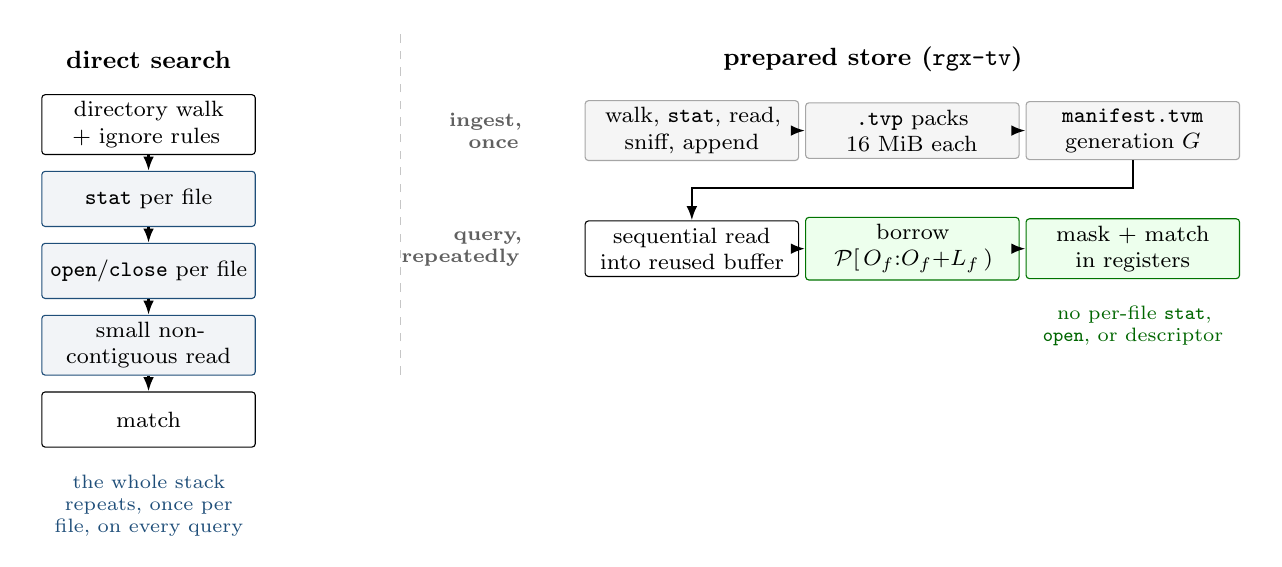
\begin{tikzpicture}[
    x=1mm, y=1mm,          % bare coordinates below are millimetres
    font=\footnotesize,
    box/.style={draw,rounded corners=1.2pt,align=center,inner xsep=3pt,
                inner ysep=2.5pt,minimum height=7mm,text width=25mm},
    cost/.style={box,draw=rgxblue,fill=rgxblue!6},
    keep/.style={box,draw=green!45!black,fill=green!7},
    once/.style={box,draw=gray!70,fill=gray!8},
    ar/.style={-{Latex[length=1.8mm]},thick},
    hd/.style={font=\small\bfseries,align=center,inner sep=2pt},
    row/.style={font=\scriptsize\bfseries,align=right,inner sep=1pt,
                text width=16mm,text=gray!75!black},
    note/.style={font=\scriptsize,align=center,inner sep=1pt,text width=30mm}
  ]
  % ---------------- left: direct search ----------------
  \node[hd] (h1) at (30,26) {direct search};
  \node[box,below=2.5mm of h1] (w1) {directory walk\\+ ignore rules};
  \node[cost,below=2mm of w1] (m1) {\texttt{stat} per file};
  \node[cost,below=2mm of m1] (o1) {\texttt{open}/\texttt{close} per file};
  \node[cost,below=2mm of o1] (r1) {small non-contiguous read};
  \node[box,below=2mm of r1] (x1) {match};
  \draw[ar] (w1)--(m1); \draw[ar] (m1)--(o1);
  \draw[ar] (o1)--(r1); \draw[ar] (r1)--(x1);
  \node[note,text=rgxblue,below=3mm of x1] {the whole stack repeats, once
        per file, on every query};

  % ---------------- right: prepared store ----------------
  \node[hd] (h2) at (122,26) {prepared store (\texttt{rgx-tv})};
  \node[row] (l1) at (69,17) {ingest,\\once};
  \node[once] (ib)  at (99,17)  {walk, \texttt{stat}, read,\\sniff, append};
  \node[once] (pk)  at (127,17) {\texttt{.tvp} packs\\16~MiB each};
  \node[once] (mf)  at (155,17) {\texttt{manifest.tvm}\\generation $G$};
  \draw[ar] (ib)--(pk); \draw[ar] (pk)--(mf);
  \node[row] (l2) at (69,2) {query,\\repeatedly};
  \node[box]  (rd)  at (99,2)  {sequential read\\into reused buffer};
  \node[keep] (sl)  at (127,2) {borrow\\$\mathcal{P}[\,O_f{:}O_f{+}L_f\,)$};
  \node[keep] (mt)  at (155,2) {mask + match\\in registers};
  \draw[ar] (rd)--(sl); \draw[ar] (sl)--(mt);
  \draw[ar] (mf.south) -- ++(0,-3.5mm) -| (rd.north);
  \node[note,text=green!40!black,below=3mm of mt] {no per-file
        \texttt{stat}, \texttt{open}, or descriptor};

  \draw[gray!45,dashed] (62,-14) -- (62,30);
  \end{tikzpicture}%
}
\caption{The two paths. Discovery and per-file metadata move out of the query
loop (left, paid once per file per query) into an amortised ingestion loop
(right, paid once). The dashed line marks the build/query boundary. Blue boxes
are the terms of \eqref{eq:direct} the pack store removes; green boxes are
what it retains; grey boxes are paid at build time only.}
\label{fig:arch}
\end{figure}

\subsection{Pack specification (\texttt{.tvp}) and generation manifest
(\texttt{manifest.tvm})}
A pack is a contiguous file targeting 16~MiB, consisting of a 32-byte
little-endian header followed immediately by unpadded payload bytes. Search
walks the payload in \emph{scan units} --- 1~MiB windows extended at both
ends to file-record boundaries (\texttt{cut\_units}) --- so a unit holds
whole slices and a file larger than a unit is searched as one contiguous
slice (\Cref{tab:boundary}). The
corpus index is a separate binary manifest, published atomically. It carries
a monotonic generation counter and a corpus fingerprint, so that a store is
invalidated when the walk configuration that produced it changes and not
only when a file does. \Cref{tab:format} gives both layouts; every integer
is little-endian.

\begin{table}[htbp]
\centering
\footnotesize
\caption{On-disk layouts. Sizes are exact and are asserted on read; a
manifest whose version is not the one this build understands is refused with
its version named rather than parsed on a guess.}
\label{tab:format}
\begin{tabular}{@{}llp{0.16\textwidth}p{0.44\textwidth}@{}}
\toprule
\textbf{Structure} & \textbf{Offset} & \textbf{Type} & \textbf{Field} \\
\midrule
\multicolumn{4}{@{}l}{\textit{Pack header (\texttt{.tvp}), 32 bytes}} \\
  & 0  & \texttt{[u8;8]}  & magic \texttt{RGXTVP01} \\
  & 8  & \texttt{u32}     & format version (1) \\
  & 12 & \texttt{u32}     & pack identifier \\
  & 16 & \texttt{u32}     & file count \\
  & 20 & \texttt{u64}     & content length (unpadded payload) \\
  & 28 & \texttt{u32}     & content CRC32 (IEEE 802.3) \\
\midrule
\multicolumn{4}{@{}l}{\textit{Manifest header (\texttt{manifest.tvm})}} \\
  & 0  & \texttt{[u8;8]}  & magic \texttt{RGXTVM01} \\
  & 8  & \texttt{u32}     & manifest version (4) \\
  & 12 & \texttt{u64}     & generation counter $G$ \\
  & 20 & \texttt{u64}     & creation timestamp (seconds) \\
  & 28 & \texttt{u64}     & corpus fingerprint \\
  & 36 & \texttt{u32}+$n$ & canonical repository root, UTF-8 \\
\midrule
\multicolumn{4}{@{}l}{\textit{Pack index record, repeated per pack}} \\
  & +0  & \texttt{u32}    & pack identifier \\
  & +4  & \texttt{u32}+$n$ & pack filename, UTF-8 \\
  & +   & \texttt{u32}    & file count \\
  & +   & \texttt{u64}    & content length \\
  & +   & \texttt{u32}    & content CRC32 \\
\midrule
\multicolumn{4}{@{}l}{\textit{File record, repeated per file}} \\
  & +0  & \texttt{u64}    & record count prefix (first record only) \\
  & +   & \texttt{u32}+$n$ & relative path, UTF-8 \\
  & +   & \texttt{u32}    & target pack identifier \\
  & +   & \texttt{u64}    & byte offset $O_i$ \\
  & +   & \texttt{u64}    & byte length $L_i$ \\
  & +   & \texttt{u64}    & modification time (seconds) \\
  & +   & \texttt{u32}    & modification time (nanoseconds) \\
  & +   & \texttt{u32}    & file CRC32 \\
  & +   & \texttt{[u64;8]} & n-gram signature, 512 bits over the text the
                            searcher sees (\Cref{sec:ngram}) \\
  & +   & \texttt{u8}     & flags: bit 0 \texttt{is\_empty}, bit 1
                            \texttt{is\_deleted}, bit 2 \texttt{is\_binary} \\
\midrule
\multicolumn{4}{@{}l}{\textit{Trailer}} \\
  & end & \texttt{u32}     & CRC32 over the whole preceding manifest \\
\bottomrule
\end{tabular}
\end{table}

Updates commit generation $G{+}1$ by writing a temporary file,
\texttt{fsync}-ing it and renaming it over the live manifest, so a concurrent
reader observes either generation $G$ in full or $G{+}1$ in full, never a
mixture. Packs are flushed before the manifest that indexes them is
published, so a published manifest never references an unflushed pack. Both
properties are exercised by the pack-store differential tests listed under
Reproducibility, which compare a prepared store against direct search on the
same corpus. The
\texttt{is\_binary} bit redefined in manifest version~3 means ``the full
content was classified at build time'', not ``an initial buffer held a
NUL''; version~4 added the per-file n-gram signature of \Cref{sec:ngram},
and a store from any other version is refused with its version named.

\subsection{Amortised binary detection}
Ripgrep decides binary-ness inside its searcher, over the bytes the
matcher is handed, on every query --- CPU spent re-deriving a constant. In
\texttt{rgx-tv} the same rule (whole content, byte-order mark decoded
first) runs once during pack construction and the verdict is stored as a
bit in the manifest. A
query then tests one bit before borrowing a slice, and the searcher disables
its own runtime binary sniffing for the same reason.

\section{Microarchitectural tier: the mask pipeline}
\label{sec:micro}
This tier takes the necessary byte conditions that \Cref{sec:foundations:cover}
places on the nibble grid and evaluates them in registers: the compilation
is proved there, and this section describes what it compiles to.

\subsection{The shape of the problem}
\label{sec:micro:shape}
A pattern's required bytes are the conjunction of one byte-class test per
position, and a bitmap is one bit per byte. The conjunction is therefore a
word-level operation over data already in L1 rather than a call per
candidate. For an alternation, the conjunction becomes a disjunction of
conjunctions. Writing the term at offset $k$ as a mask of the haystack
shifted by $k$,
\begin{align}
\label{eq:oran}
M_{\texttt{pub}} &= P \mathbin{\&} (U{\gg}1) \mathbin{\&} (B{\gg}2)
                    \mathbin{\&} (\mathit{Sp}{\gg}3) \mathbin{\&} (\mathit{Lc}{\gg}4) \notag\\
M_{\texttt{fn}}  &= F \mathbin{\&} (N{\gg}1) \mathbin{\&} (\mathit{Sp}{\gg}2)
                    \mathbin{\&} (\mathit{Lc}{\gg}3) \notag\\
M &= M_{\texttt{pub}} \mid M_{\texttt{fn}} .
\end{align}
The bitmap names are local to this display and stand for the bytes they
test: $P,U,B$ the letters of \texttt{pub}, $F,N$ the letters of
\texttt{fn}, $\mathit{Sp}$ the separating space, $\mathit{Lc}$ the combined
lowercase-class term at the first letter position. This is an \emph{OR of
ANDs} --- a monotone Boolean formula over the
necessary-condition tests, which is precisely the positive normal form of
the sound abstraction of \Cref{sec:foundations:abs}. There is no complement
anywhere in it, and it is worth being explicit about that, because the
natural but incorrect picture is a forward candidate mask intersected with
an inverted secondary mask. The engine never forms such a pair: a secondary
constraint such as the \texttt{[a-z]} of \texttt{(pub|fn) [a-z]+} is
absorbed at compile time into one combined class at its own offset, and the
accumulator is narrowed by positive class tests only.

\subsection{Class-partitioned nibble decomposition}
The cost of \eqref{eq:oran} is dominated by how a class test is performed,
and \Cref{prop:cover} is the whole story: the class is compiled to its
row-pattern cover on the $16\times16$ nibble grid, each distinct row mask
becomes one bit-plane, and one \texttt{vpshufb} pair evaluates the OR of
the planes bit-parallel. A class of arbitrary width with $k\le 8$ distinct
row patterns costs exactly one shuffle pair; a class with $k>8$ is refused
at compile time and falls back to scalar. The nibble pair is a lookup, not
a comparison, so the marginal cost of a class term is one \texttt{vpshufb}
against four \texttt{vpcmpeqb} for a single-byte term --- which is why
single-byte terms are split out ahead of class terms and run as a separate
straight loop.

\subsection{The kernel}
\Cref{fig:mask} shows the pipeline. The inner loop processes 64 bytes per
iteration; for each branch it ANDs one term at a time into an accumulator,
ORs the branches together, and stores one \texttt{u64}.

\begin{figure}[t]
\centering
\resizebox{\textwidth}{!}{%
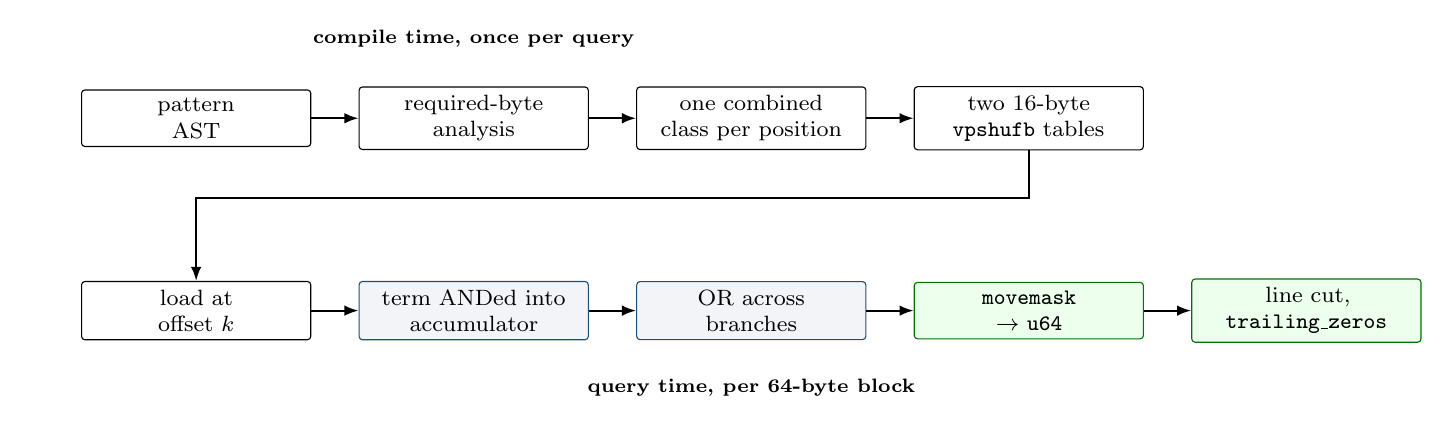
\begin{tikzpicture}[
    font=\footnotesize,
    box/.style={draw,rounded corners=1.2pt,align=center,inner sep=3pt,
                minimum height=7mm,text width=27mm},
    hot/.style={box,draw=rgxblue,fill=rgxblue!6},
    sink/.style={box,draw=green!45!black,fill=green!7},
    ar/.style={-{Latex[length=1.8mm]},thick},
    stage/.style={font=\scriptsize\bfseries,align=center,inner sep=1pt}
  ]
  % ---- compile time
  \node[stage] (c0) at (0,0) {};
  \node[box,right=6mm of c0] (ast) {pattern\\AST};
  \node[box,right=6mm of ast] (req) {required-byte\\analysis};
  \node[box,right=6mm of req] (cls) {one combined\\class per position};
  \node[box,right=6mm of cls] (tab) {two 16-byte\\\texttt{vpshufb} tables};
  \node[stage,above=4.5mm of req] {compile time, once per query};
  % ---- query time
  \node[box,below=17mm of ast] (ld) {load at\\offset $k$};
  \node[hot,right=6mm of ld] (tm) {term ANDed into\\accumulator};
  \node[hot,right=6mm of tm] (br) {OR across\\branches};
  \node[sink,right=6mm of br] (mm) {\texttt{movemask}\\$\rightarrow$ \texttt{u64}};
  \node[sink,right=6mm of mm] (cut) {line cut,\\\texttt{trailing\_zeros}};
  \node[stage,below=4.5mm of br] {query time, per 64-byte block};
  \draw[ar] (ast) -- (req);
  \draw[ar] (req) -- (cls);
  \draw[ar] (cls) -- (tab);
  \draw[ar] (tab.south) -- ++(0,-6mm) -| (ld.north);
  \draw[ar] (ld) -- (tm);
  \draw[ar] (tm) -- (br);
  \draw[ar] (br) -- (mm);
  \draw[ar] (mm) -- (cut);
  \end{tikzpicture}%
}
\caption{The compiled mask pipeline. A pattern's required bytes are analysed
and folded into one combined byte class per position offline, so the
per-query work is a fixed sequence of ANDs. At query time each term is ANDed
into a vector accumulator, the branches are ORed, and a single word per
64-byte block reaches the line cut. No scalar confirmation occurs on this
path, and no branch is taken per candidate --- the one data-dependent
branch is the block-level skip of an already-empty accumulator.}
\label{fig:mask}
\end{figure}

The kernel is shown in \Cref{code:kernel}. Two details carry most of the
benefit. First, a term at offset $k$ is evaluated by \emph{loading} the
haystack $k$ bytes further along rather than by shifting a mask: lane $m$ of
that load is already byte $\text{base}+k+m$, so a real shift would move the
bit twice. This is why the block is 64 bytes rather than 32 --- a 32-byte
block would have to be stitched across blocks to cover the 31 positions a
shifted term reaches back over. Second, after the cheap single-byte terms,
if the accumulator is already zero for all 64 bytes the expensive
\texttt{vpshufb} terms are skipped entirely --- ANDing further terms cannot
revive a zeroed accumulator --- and the same test stops the class-term run
mid-way at the first zeroing. The skip fires on blocks where the cheap
conjunction has no survivor at all: for a high-frequency single-byte term
that is the rare case (a 7\% byte is present in about 99\% of 64-byte
blocks), and for a rare multi-byte conjunction it is the common one. The
term it avoids paying is the shuffle pair of every remaining class term of
that branch.

\begin{lstlisting}[
  caption={The AVX2 mask fill, reduced to its essential structure. Two
  32-byte halves per iteration, one accumulator per branch, branches ORed,
  one \texttt{u64} stored.},
  label={code:kernel},
  language={Rust}]
#[target_feature(enable = "avx2")]
unsafe fn avx2_match_bits(plan: &MatchMask, hay: &[u8], out: &mut BitMap) {
    for b in &plan.branches {
        let ops = &plan.ops[b.start as usize..b.start as usize + b.len as usize];
        let mut acc_lo = _mm256_set1_epi8(-1);
        let mut acc_hi = _mm256_set1_epi8(-1);
        let mut dead = false;

        // one-byte terms: a broadcast compare
        for (idx, o) in ops[..b.split as usize].iter().enumerate() {
            let p = hay.as_ptr().add(base + o.shift as usize);
            let a = _mm256_loadu_si256(p as *const __m256i);
            let a2 = _mm256_loadu_si256(p.add(32) as *const __m256i);
            acc_lo = _mm256_and_si256(acc_lo, _mm256_cmpeq_epi8(a, vec));
            acc_hi = _mm256_and_si256(acc_hi, _mm256_cmpeq_epi8(a2, vec));
        }

        // class terms are only worth their shuffle pair if the
        // accumulator is not already empty across the whole block
        if (b.split as usize) < ops.len() {
            let or_all = _mm256_or_si256(acc_lo, acc_hi);
            if _mm256_testz_si256(or_all, or_all) == 1 { dead = true; }
        }

        if !dead {
            for o in &ops[b.split as usize..] {
                let p = hay.as_ptr().add(base + o.shift as usize);
                let a  = _mm256_loadu_si256(p as *const __m256i);
                let a2 = _mm256_loadu_si256(p.add(32) as *const __m256i);
                let m_a  = lookup(a,  tl, th, k0f);   // lo[l] & hi[h]
                let m_a2 = lookup(a2, tl, th, k0f);
                // AND in class MEMBERSHIP, expressed as the complement
                // of a non-membership compare -- not an inverted
                // secondary mask
                acc_lo = _mm256_andnot_si256(_mm256_cmpeq_epi8(m_a,  zero), acc_lo);
                acc_hi = _mm256_andnot_si256(_mm256_cmpeq_epi8(m_a2, zero), acc_hi);
            }
            res_lo = _mm256_or_si256(res_lo, acc_lo);
            res_hi = _mm256_or_si256(res_hi, acc_hi);
        }
    }
    out.push64(base, lanes(res_lo) | (lanes(res_hi) << 32));
}
\end{lstlisting}

What bounds the loop is its read window: a block is admitted only when its
full window --- $63+w$ bytes from the block's base, with $w$ one past the
last byte any term reads --- lies inside the haystack, and the remaining
tail, the last $w+62$ bytes, is evaluated by the scalar predicate, which is
the definition the vector fill implements rather than an approximation of
it. No load crosses the haystack bound. That is what licenses invariant~1
of \Cref{thm:equivalence} on the scan layer: inside a borrowed slice, the
vector path never touches a byte outside $[O_f,O_f+L_f)$, and a file larger
than a block is stitched nowhere --- it is one haystack.

The dispatch is at runtime, not compile time. One binary is shipped to
arbitrary machines, so the vector fill is entered behind
\path{is_x86_feature_detected!} in the order AVX-512BW, then AVX2, with a
scalar implementation of the identical predicate as the definition and the
fallback. \Cref{code:kernel} is the AVX2 fill; the AVX-512BW fill computes
the same predicate set, evaluating each single-byte term as one
\texttt{vpcmpb} mask and keeping the class lookup on the same nibble
tables. Which fill a timing ran is a property of its host: the primary
host's Zen~4 core exposes AVX-512BW, so its numbers are that fill of the
same predicate. The claims of this paper attach to the predicate set
(\Cref{thm:fnr}, and a differential suite pinning the fills against the
scalar definition) and to the end-to-end pipeline, not to one instruction
sequence.

\subsection{Candidate suppression and the meaning of diodicity}
\label{sec:dio}
For a pattern with a high-frequency prefix, the quantity of interest is the
ratio of naive prefix candidates to offsets the compiled predicate set
admits --- the mask's fixed-offset terms and, where the pattern has one,
its trailing-literal check. We call
it the \emph{diodicity} in the sense of \eqref{eq:di}: the ratio of
resistance presented to the reverse (non-matching) direction to that
presented to the forward (matching) direction. In circuit language the mask
is a half-wave rectifier: forward current (true matches) passes with
$\mathrm{FNR}=0$ guaranteed by \Cref{thm:fnr}, reverse current (noise
candidates) is suppressed in place at zero branch cost.

\Cref{tab:dio} reports it. The measurement harness evaluates each shape's
predicate in scalar reference form --- the mask's terms for the fixed-offset
shapes, the trailing-literal check for the pair --- so the ratios are
properties of the predicate set and not of the vector loop: the production
AVX2 kernel computes the same set, which is the content of
\Cref{thm:fnr}. The harness reports true hits rather than a false-negative
count, because a scalar reference evaluation of the same predicate cannot
disagree with itself; the false-negative guarantee is established by
\Cref{thm:fnr} and by the differential suite, not by this table.

\begin{table}[htbp]
\centering
\footnotesize
\caption{Candidate-suppression ratio of the compiled predicate set,
measured over \texttt{big235.rs} (246{,}541{,}116~bytes,
sha256:\texttt{9c38d37f\ldots}). ``Quenched'' is the fraction of naive
high-frequency prefix candidates eliminated before scalar confirmation.
The predicate admits a subset of the naive candidate set by construction,
so no false negatives arise; see \Cref{thm:fnr}. The scalar reference
bounds the pair row's suffix search at 1{,}024~bytes where production
searches the rest of the line; on this corpus the bound changes no answer.}
\label{tab:dio}
\begin{tabular}{@{}llrrr@{}}
\toprule
\textbf{Pattern} & \textbf{Constraint shape}
  & \textbf{Naive candidates} & \textbf{Admitted} & \textbf{Quenched} \\
\midrule
\texttt{e[0-9]}          & literal $\times$ class
  & 16{,}136{,}619 & 240{,}786    & \textbf{98.51\%} \\
\texttt{foo.*bar}        & literal $\times$ sparse literal pair
  & 528{,}058      & 264{,}029    & \textbf{50.00\%} \\
\texttt{(pub|fn) [a-z]+} & alternation $\times$ class
  & 2{,}264{,}327  & 2{,}105{,}177 & \textbf{7.03\%} \\
\bottomrule
\end{tabular}
\end{table}

The ordering is the informative part. Suppression is largest exactly where
the secondary constraint is most selective --- one digit class after a very
common letter --- and nearly worthless when the naive literal is already rare
(\texttt{foo}), or when the branch set is an alternation of two short
literals that together cover most occurrences. The technique pays for dense
prefixes and does nothing for sparse ones. This is the rectifier's operating
point: diodicity is a property of the \emph{constraint's} asymmetry, not of
the silicon, and a pattern whose naive candidate stream is already clean
buys the architecture nothing at this tier.

The sparse row is at that tier's ceiling rather than short of it: the
264{,}029 candidates it admits are exactly the 264{,}029 positions where
\texttt{foo.*bar} matches, so 50.00\% quenched is everything the shape
gives, and no anchoring of the second literal --- at any distance --- could
admit fewer on this corpus. The exact 2:1 ratio of the counts
(528{,}058 against 264{,}029) is a property of this corpus and not of the
predicate; the ceiling claim is corpus-bound, and a second corpus is the
natural check (\Cref{sec:future}).

\subsection{A second, distinct filter: n-gram signatures}
\label{sec:ngram}
An orthogonal mechanism prunes whole files before any slice is borrowed. Each
file is summarised at build time by a signature over contiguous 4-grams
(stride 1): two independent hash functions --- a forward and a reverse
FNV-variant seeded differently and mixed with the background byte rank ---
map each admissible gram to one bit each in separate halves of the summary,
so a 256-bit signature is a \emph{partitioned two-hash Bloom filter}
\cite{bloom1970} of $m=256$, $k=2$, split into two 128-bit halves so the
forward and reverse directions never collide; the 512-bit variant widens
each half to 256 bits. Grams whose background-frequency cost exceeds a
noise threshold (runs of whitespace-class common bytes) are not inserted at
all, so the effective insertion count $n$ is a rarity-weighted quantity,
not $L-3$. A query is admitted into a file only if the query's signature
bits are a subset of the file's --- the standard Bloom subset test, which
is a superset filter: a false positive costs only a slice search, a false
negative would be a lost match, and the stride-1 insertion of every
admissible gram makes the latter impossible by construction (the harness
verifies zero false negatives).

Soundness on the query side is a statement about which bytes a pattern
\emph{requires}, not about how it is spelled. The query signature covers
the literal every match of the pattern contains --- from the
necessary-condition analysis of \Cref{sec:foundations:cover}, the same one
the mask pipeline compiles --- because a spelling is not required of a
match: \texttt{abcd|efgh} matches a file holding one branch, and
\texttt{abcd*} matches \texttt{abc}, so a signature read off the pattern's
text would prune files that match. The stored signature covers the bytes
the searcher will actually see, so a byte-order-marked file is signed as
its decoded form rather than as its interleaved encoding. And the filter
stands down --- every file is searched, never none --- whenever the
requirement is weaker than the test: a case-folded literal (the stored
signature is case-sensitive), a pattern with no required literal of four
bytes, a forced input encoding, an inverted query, or a file an adapter
claims. An all-zero signature is ``unknown'' --- an archive member, an
empty file --- and never rejects. A caller that reads ``no filter'' as
``no match'' loses files, which is the one failure this construction
forbids.

\Cref{tab:ngram} reports the fraction of
files \emph{pruned} by the filter over 15{,}000 files of the Cargo
registry; the admitted fraction is the complement.

\begin{table}[htbp]
\centering
\footnotesize
\caption{N-gram signature filter, prune efficiency in per cent (files
eliminated before a slice is borrowed; the admitted fraction is the
complement). Two runs of the same harness (tree \texttt{36e3307}, blob
\texttt{42a67f68\ldots}) over one corpus: 15{,}000 \texttt{.rs} files
harvested by content digest (\texttt{sha256:b6b01945\ldots}, 337.66~MB),
so the two runs count the same files to the byte and every prune figure
agrees exactly. Latency is per file evaluated in one timer scope on both
hosts. Zero false negatives on every row of every run.}
\label{tab:ngram}
\begin{tabular}{@{}lcccc@{}}
\toprule
& \multicolumn{2}{c}{\emph{Run A --- Windows}} & \multicolumn{2}{c}{\emph{Run B --- CachyOS}} \\
\cmidrule(lr){2-3}\cmidrule(lr){4-5}
\textbf{Pattern} & 256-bit & 512-bit & 256-bit & 512-bit \\
\midrule
\multicolumn{5}{@{}l}{\emph{Pruned (count)}} \\
\texttt{fn main}  & \textbf{17.23\%} (2{,}585) & \textbf{29.97\%} (4{,}495)
                  & \textbf{17.23\%} (2{,}585) & \textbf{29.97\%} (4{,}495) \\
\texttt{pub fn}   & \textbf{13.25\%} (1{,}987) & \textbf{24.30\%} (3{,}645)
                  & \textbf{13.25\%} (1{,}987) & \textbf{24.30\%} (3{,}645) \\
\texttt{let mut}  & \textbf{16.51\%} (2{,}476) & \textbf{29.33\%} (4{,}399)
                  & \textbf{16.51\%} (2{,}476) & \textbf{29.33\%} (4{,}399) \\
\texttt{struct }  & \textbf{11.71\%} (1{,}757) & \textbf{22.27\%} (3{,}340)
                  & \textbf{11.71\%} (1{,}757) & \textbf{22.27\%} (3{,}340) \\
\midrule
\multicolumn{5}{@{}l}{\emph{Filter latency (ns/file)}} \\
\texttt{fn main}  & 3.02 & 4.31 & 4.38 & 5.61 \\
\texttt{pub fn}   & 2.20 & 4.23 & 2.49 & 4.81 \\
\texttt{let mut}  & 2.76 & 4.25 & 2.65 & 6.65 \\
\texttt{struct }  & 2.10 & 6.06 & 2.51 & 7.08 \\
\bottomrule
\end{tabular}
\end{table}

Both runs agree on the only ordering the construction predicts: the
512-bit filter prunes \emph{strictly more} files than the 256-bit filter
on every pattern (22.3--30.0\% against 11.7--17.2\%), with zero false
negatives throughout. The corpus being one set of bytes, the two runs
report identical counts rather than near ones. That
is the direction of the idealised Bloom model
$p_{\mathrm{fp}}=(1-e^{-kn/m})^{k}$, which decreases with $m$ at fixed $n$
and $k$: a wider signature is a stronger filter. The 256-bit filter
eliminates 12--17\% of the corpus before a byte is read; the 512-bit
filter eliminates 22--30\%.

What the table reports is the prune rate; what it does not report is the
Bloom \emph{false-positive rate} --- the share of admitted files that carry
the required grams but not the pattern --- because the harness counts
prunes, not matches. The admitted side of these rows (83--88\% at 256-bit,
70--78\% at 512-bit) is therefore dominated by false-positive admission
whenever the pattern is rarer than the four-byte grams it requires, and
each false positive costs one slice search and nothing more. That is the
whole economics of a superset filter and it is why the per-file test is
kept at two word ANDs: the filter is cheap and weak rather than selective,
and the claim made for it is the measured prune rate, not an idealised
$p_{\mathrm{fp}}$.

\subsection{A reporting error, not an empirical mystery}
\label{sec:ngram:inversion}
A mislabelled transcription of this harness reports the opposite of the
paragraph above: 512-bit ``admitting'' 22--30\% of files against
256-bit's 12--17\%, which contradicts the textbook model and invites a
mechanism --- weakly-avalanched half-selector, collision structure
changing with $m$ --- that no measurement supports. The harness prints
three columns: files admitted, files pruned, and prune efficiency. A
transcription that copies the \emph{pruned} count into a column labelled
``admitted'' inverts the finding without changing a single measurement.
The \texttt{fn main} row shows both sides of the one number: 2{,}585
files pruned at 17.23\% and 12{,}415 admitted at 82.77\%, identically on
both hosts. A filter output has an admitted side and a pruned side; they
are complements, and a table must name which one it prints. The
construction is not the ideal triple --- the insertion set is
rarity-thresholded and the two directions occupy disjoint halves of the
same weakly-avalanched hash --- but nothing in these runs requires any of
that to explain the ordering. Widening the signature strengthens the
filter; both hosts say so, in identical counts.

The two residuals this measurement carries are named and closed by the
corpus and the timer it declares. The prune rates come from one
digest-named corpus (\path{scripts/harvest-ngram-corpus.py}; both runs
print its \texttt{sha256:b6b01945\ldots}), so the counts agree to the file
rather than by subset luck, and the latency column comes from one timer
scope on both hosts (2.1--6.1~ns against 2.5--7.1~ns per file), which is
the direction of the machines' relative speed. The prune rates are the
standalone harness's; the shipped
filter runs the same signatures on the query path, where the per-file test
is two word ANDs before the slice is borrowed. \Cref{tab:ngram} measures the
filter on its own and \Cref{sec:ablations} runs it end to end, where its effect
does not rise above the harness floor (\Cref{sec:limits}).

\section{The memory-mapping paradox}
\label{sec:mmap}

\subsection{The in-process measurement illusion}
A common belief is that memory-mapped I/O is universally superior to buffered
streaming for read-heavy workloads because it avoids a user-space copy. In
\texttt{rgx-tv} the belief fails on the wall clock, and an in-process timer
is the reason it looks otherwise: an experimental flag that skips the
user-space unmap --- the leaked arm of \Cref{tab:unmap} --- reports 53.9\%
less in-process time than the same mapping under explicit unmap. The
improvement is teardown accounting, not anything mapping does to the search.

\begin{table}[htbp]
\centering
\footnotesize
\caption{In-process profiling against external wall clock. Stage times
overlap the total, since setup and teardown are measured independently of
the search stage; the point is the discrepancy between the two accounting
methods, not a partition of the total.}
\label{tab:unmap}
\begin{tabular}{@{}lrrrr@{}}
\toprule
\textbf{Configuration} & \textbf{In-process} & \textbf{Search}
  & \textbf{Teardown} & \textbf{Wall clock} \\
\midrule
\texttt{mmap} (explicit unmap) & 306.7~ms & 108.8~ms & 167.4~ms & 342.1~ms \\
\texttt{mmap} (leaked)         & 141.5~ms & 110.3~ms & \textbf{0.0~ms} & 348.9~ms \\
\bottomrule
\end{tabular}
\end{table}

Measured externally on the command-line wall clock across 11 paired rounds,
leaking the mapping produced no speedup at all (+2.0\%, within noise). The
cause is that skipping the user-space unmap does not remove the work, it
defers it: at process exit the kernel must still walk page tables and tear
down mappings for all 117 packs before returning control to the terminal.
This is an observer-effect of the measurement apparatus, in the plain
sense and in the sense catalogued by \cite{mytkowicz2009}: the in-process timer is inside the system it measures and stops
before the system is finished, so it reports the deferred work as deleted
work. The discipline this imposes is the project's harness rule
generally --- the estimator must sit outside the boundary of the effect,
and an in-process stage timer cannot adjudicate a claim about end-to-end
latency.

\subsection{Page-fault cost during execution}
The cost is not confined to teardown. Mapping 1.87~GB across 117 packs leaves
the pages unpopulated, and each 4~KiB page a worker touches raises a hardware
page-fault exception --- roughly 480{,}000 across the corpus --- serialising
kernel trap handling and contending on page-table locks across cores. In the
transport picture of \Cref{sec:model}, every fault is a scattering centre in
the byte stream: the mapping converts a smooth $\beta$ term into
$B/\beta + N_{\text{pages}}\cdot c_{\text{fault}}$ with a syscall-class
constant $c_{\text{fault}}$, which is exactly the ballistic term the pack
store was built to remove. A mapping is therefore not free of
\eqref{eq:direct}; it relocates some of $\sigma N$ into the page-fault
integral.

\subsection{Resolution: wire-speed sequential streaming}
The default is therefore sequential chunk streaming.
Each worker claims a pack through an atomic counter, reads it into a
thread-local buffer allocated once and reused, and searches the borrowed
slices in place. What the streaming path avoids is the per-pack mapping and
teardown the mmap arm pays: no page table is populated for pack bytes and none
is torn down afterwards, and the buffer each worker holds is allocated once and
reused across its claims. \Cref{tab:nine} measures the result as a full factorial design
over three thread counts and three pattern classes.

\begin{table}[htbp]
\centering
\footnotesize
\caption{``Parallel'' sequential chunk streaming (\texttt{ParallelBuffered})
against memory mapping: paired median latency delta in per cent, negative
favouring streaming. Three thread counts by three pattern classes, 11 paired
rounds with order rotation, $\pm 2\%$ floor, on the digest-pinned
93{,}234-file corpus (\texttt{seed 0x5eed1234abcd0001}, 1.89~GB, 114 packs;
\texttt{benchmark/tv-matrix-transcript.md}). Eight of nine cells separate
under the distribution gate; the \texttt{-j1} \texttt{pub fn} row overlaps
with streaming's median $25.9\%$ below mapping's.}
\label{tab:nine}
\begin{tabular}{@{}llcccc@{}}
\toprule
\textbf{Class} & \textbf{Pattern}
  & \textbf{\texttt{-j1}} & \textbf{\texttt{-j8}} & \textbf{\texttt{-j32}}
  & \textbf{Overlap} \\
\midrule
High frequency & \texttt{pub fn} (\texttt{-c}, 6{,}781{,}133) & $-$25.9\% (overlap) & $-$\textbf{56.1\%} & $-$\textbf{54.0\%} & \texttt{-j1} only \\
I/O floor      & \texttt{nonexistent\_token\_xyz} (\texttt{-c}, 0) & $-$\textbf{43.5\%} & $-$\textbf{61.1\%} & $-$\textbf{67.3\%} & none \\
Full output    & \texttt{fn main} (full, \texttt{md5:1772dc8575f1}) & $-$\textbf{9.8\%} & $-$\textbf{11.2\%} & $-$\textbf{11.2\%} & none \\
\bottomrule
\end{tabular}
\end{table}

Every separated cell favours streaming, and the matrix settles what an
earlier unpinned run's single $-44.3\%$ mean obscured: \emph{the magnitude
of the read-mode gap is cell-dependent}. The scan-bound count rows at this
scale land at $-43.5\%$ to $-67.3\%$ (reproducing the earlier $-44.3\%$
figure to within a point on the \texttt{-j1} I/O-floor row, and widening at
\texttt{-j8}/\texttt{-j32} where page-table lock contention grows), while
the output-bound full row lands at $-9.8\%$ to $-11.2\%$ across all thread
counts --- where serialisation owns a larger share of the wall clock. That
cell split reconciles the second host's paired probe (Linux, Ryzen~7~255;
\Cref{sec:eval:cross}), which measured \texttt{fn main} over the
20{,}000-file benchmark tree and found streaming faster than mapping on
every paired round by 3--18\% (mean $\approx 12\%$), with serial buffered
reads $\approx 8\times$ slower than either (and 34--52\% slower than
mapping at \texttt{-j8}/\texttt{-j32} here). Both numbers were measuring
their own cell: a bare ``$-44.3\%$'' and a bare ``$\approx 12\%$'' are each
incomplete without the cell attached (\Cref{sec:limits}), and a re-run of
the count rows on the smaller 20{,}000-file tree returned ``overlap, not a
result'' under the distribution gate. What the two hosts establish together
is that the \emph{direction} is not a Windows artefact and the
\emph{magnitude} is set by the cell and corpus scale: buffered streaming
beats memory mapping on a one-shot query every time it separates, backed by
the 93k factorial, the 480{,}000-fault accounting, the phantom-unmap
experiment of \Cref{tab:unmap} (and its $-j8$ counterpart in
\path{benchmark/tv-matrix-transcript.md}, where teardown is 186.3~ms of a
384.2~ms in-process total and zero of the wall clock), and the cross-host
pairing.

\section{Evaluation}
\label{sec:eval}

\subsection{Setup}
All measurements were taken on a dedicated system under locked clocks:
AMD~Ryzen~9 7950X3D (16 physical cores, 32 threads, 128~MB 3D V-Cache),
64~GB DDR5-6000 CL30, Kingston FURY~Renegade~G5 4~TB PCIe~5.0 NVMe
(SFYR2S4T0, system drive), Windows~11~Pro build 26100,
\texttt{rustc}~1.98.1. Baselines are Vanilla Ripgrep 15.0.0
(rev \texttt{3a612f88b8}), direct \texttt{rgx} and prepared
\texttt{rgx-tv}, measured from one release build of the same tree.

Three protocol rules govern every timing line, and a measurement that
violates them is not reported. First, comparisons are \emph{thread-matched}:
both engines are given the same \texttt{-j} value, printed in the header,
because ripgrep caps its own default at
$\min(\mathrm{available\_parallelism()},12)$ and an uncapped comparison
compares thread counts rather than code. Second, a \emph{count gate} runs in
front of each timing: the summed \texttt{-c} of the two engines on the same
corpus must agree, or the line is suppressed, so that a faster time cannot be
a smaller result. Third, a \emph{verdict that can refuse}: inside a $\pm3\%$
floor a row is a tie, outside it a winner is named only if every sample of
one engine lies below every sample of the other, and overlapping
distributions are reported as such rather than as a ratio. The pack-store
tables below additionally rotate the arm order within each paired round and
report the minimum of seven paired samples per arm
(\path{scripts/tv-vs-rg.sh}); absolute milliseconds drift across sessions
on this machine, so ratios are the claim and the counts are the invariant.

\paragraph{What the estimator is, and what the cache was.}
The pack-store columns are the \emph{minimum} of seven paired samples per
arm, which estimates the uncontended floor of a warm run and not its mean;
the spread across rounds lives in the transcripts, not in the tables. The
tables therefore print point estimates without error bars; the uncertainty
instrument is the distribution gate --- a separation verdict per row --- and
a ratio appears only where the gate named a winner. The
timer is the shell's wall clock around the whole process --- setup, search
and teardown --- with query output discarded, and the count gate runs in a
separate untimed pass so the harness's own output I/O is charged to no arm.
No cache drop is performed between rounds: the untimed pass and the first
round populate the page cache, so every latency reported in the tables is a
\emph{warm-cache} number. The cold regime is measured once, on the second
host, with each sample preceded by \texttt{sync} and
\texttt{drop\_caches} (\path{benchmark/cold-transcript-linux.md}): the
store's first cold query costs 54--56~ms against 50--51~ms warm
($+8\%$), because 26 sequential pack reads are cheap to bring in, while
the direct arms pay $+30\%$ re-reading 20{,}000 metadata records (101 vs
76~ms in-house; 88 vs 63~ms ripgrep) --- and the cold store answers
faster than the warm ripgrep arm. A first query over a cold store is
therefore bounded by the store's query-path floor of \Cref{sec:eval:cargo} and by
little else. The estimand is wall-clock time a user waits, not process CPU time,
and no stage timer is used to adjudicate an end-to-end claim
(\Cref{sec:mmap} is the case study of why not). Within a table every arm
runs on the same machine at the same frequency, ripgrep is one version
(15) throughout with identical flags across arms, and the warm-up is
defined: the untimed count pass and the first round populate the page
cache, and no round is measured before them.

\paragraph{What is compared, and what is not.}
The baselines are ripgrep and the in-house direct engine, and the rows
compared are their common denominator: a pattern in, matching lines and
counts out. The fourth arm has since been run: \texttt{ugrep}~7.8.5
\cite{ugrep} under the same gate is the slowest of the four on the fixed
tree (266--298~ms against 134--154~ms for ripgrep and 55--67~ms for the
store, counts equal on every pattern; \path{benchmark/ugrep-transcript.md}).
Still not run: a memory-mapped direct path, an
inverted or n-gram index at query time, or a database full-text index ---
each is a reasonable fifth arm and none appears in this paper. At the
engine level the comparison is already in the tables: the Direct rgx arm
runs against ripgrep's own vectorised literal prefilters --- the packed
SIMD lineage of \cite{qiu2021teddy} --- so the compiled mask is measured
against a production SIMD matcher and not against a scalar strawman. The
feature sets are not identical, and saying so costs the tables nothing:
ripgrep re-evaluates ignore rules and sniffs for binary content on every
query, while \texttt{rgx-tv} answers from what was ingested (ignore policy
and binary verdict fixed at build), never re-walks, and surfaces
adapter-rendered container text by running the same adapter pipeline over
each borrowed slice that the direct path runs over the file
(\texttt{--tv-pre-extract} moves that extraction to build time). What holds
by construction is parity between the store and the \emph{direct engine} ---
\Cref{thm:equivalence}, extraction pipeline included --- which is what makes
a store-vs-direct ratio a ratio between the same result. Parity with
ripgrep, where the tables show it, is empirical and enforced by the count
gate: the two engines can disagree on adapter-rendered container text
(ripgrep never reads it) and wherever their binary verdicts differ, and
\Cref{sec:limits} names both boundaries.

\subsection{Fixed benchmark corpus (20{,}000 files, 417.7~MB)}
\label{sec:eval:tree}
The corpus is the generated tree produced by
\path{scripts/make-corpus.py} into \path{~/.rgx-bench/tree}: 20{,}000
Rust source files whose ingestion fills 26 packs of 417{,}730{,}136 payload
bytes; the walk itself visits 20{,}028 entries, the remainder being the
store's own files. The pack store was rebuilt for this measurement in
$T_{\text{build}} = 2.26$~s and is queried at \texttt{-j32}. All three
arms agree on every match count (the count gate passes every row), and
the numbers below are one self-contained paired run of 2026-10-11 ---
\emph{one} harness, \emph{one} store, all three arms interleaved per round
--- rather than columns stitched from different sessions.

\begin{table}[htbp]
\centering
\footnotesize
\caption{Query latency on the 20{,}000-file fixed corpus at \texttt{-j32},
minimum of 7 paired rounds with order rotation. Match counts are identical
across ripgrep, direct rgx and rgx-tv on every row (count gate). The
2026-10-10 run of the same protocol measures 56--109~ms for the pack
column against a slower ripgrep arm; the cross-session spread is discussed
in \Cref{sec:limits}.}
\label{tab:small}
\begin{tabular}{@{}lrrrrrr@{}}
\toprule
\textbf{Pattern} & \textbf{Matches} & \textbf{rg 15} & \textbf{Direct rgx}
  & \textbf{rgx-tv} & \textbf{tv vs.\ rg} & \textbf{tv vs.\ rgx} \\
\midrule
\texttt{a|b|c}      & 10{,}201{,}075 & 145~ms & 127~ms & \textbf{47~ms} & \textbf{3.09$\times$} & \textbf{2.70$\times$} \\
\texttt{e}          & 11{,}764{,}155 & 143~ms & 121~ms & \textbf{46~ms} & \textbf{3.11$\times$} & \textbf{2.63$\times$} \\
\texttt{e.}         & 11{,}739{,}023 & 148~ms & 129~ms & \textbf{53~ms} & \textbf{2.79$\times$} & \textbf{2.43$\times$} \\
\texttt{pub fn}     &  1{,}492{,}934 & 137~ms & 118~ms & \textbf{46~ms} & \textbf{2.98$\times$} & \textbf{2.57$\times$} \\
\texttt{fn main}    &    297{,}851 & 129~ms & 124~ms & \textbf{41~ms} & \textbf{3.15$\times$} & \textbf{3.02$\times$} \\
\texttt{let mut}    &     67{,}616 & 132~ms & 119~ms & \textbf{39~ms} & \textbf{3.38$\times$} & \textbf{3.05$\times$} \\
\texttt{e[0-9]}     &    406{,}122 & 136~ms & 119~ms & \textbf{41~ms} & \textbf{3.32$\times$} & \textbf{2.90$\times$} \\
\texttt{(pub|fn) [a-z]+} &  2{,}091{,}372 & 140~ms & 119~ms & \textbf{47~ms} & \textbf{2.98$\times$} & \textbf{2.53$\times$} \\
\bottomrule
\end{tabular}
\end{table}

Range against ripgrep: \textbf{2.79--3.38$\times$}; against the in-house
direct engine: \textbf{2.43--3.05$\times$}. The mean query costs over the
minima as printed are
$\bar{T}_{\text{rg}} = 138.8$~ms, $\bar{T}_{\text{rgx}} = 122.0$~ms and
$\bar{T}_{\text{tv}} = 45.0$~ms, so \Cref{thm:breakeven} gives
\begin{equation}
Q^{*} = \frac{2{,}257.5}{138.8-45.0} \approx 24.1
\end{equation}
queries against ripgrep and $2{,}257.5/(122.0-45.0)\approx 29.3$ against
the direct engine --- both well inside a working session of recurrent
search over a fixed tree.

Two anchors frame the regime picture so it is not
understated. At the small-corpus end the ratio is at its widest and
compresses as the corpus grows, because \eqref{eq:twoterm-tv}'s
$N$-coefficient is negligible and its bandwidth term scales with $B$, while
the direct arms improve
with parallelism --- the shape \Cref{prop:separation} predicts. The
widest ratios live in that small-corpus regime; the project quotes no
number from it here, because no run in that regime is filed under the
protocol of \Cref{sec:eval} and a figure without its harness is not a
measurement. And the
\emph{single-file} end of the same axis (246~MB, one file, no walk) is
where the in-house \emph{engine} can lead ripgrep --- by 33--114\% on the
primary host here, by 20--40\% on two shapes and trailing on six of nine
on a second host (\Cref{sec:eval:cross}). That measurement belongs to the
matcher, not to the store, and the two must not be quoted as one number;
the matcher margin itself is not portable and is treated as such below.

\paragraph{Direct rgx versus ripgrep on this corpus is parity-to-slight-lead.}
Every ``Direct rgx'' row is faster than its ``rg 15'' row, by 5 to 22~ms on a
129--148~ms baseline --- a 4 to 15\% lead, which the store's 86 to 107~ms
advantage over the same baseline exceeds on every row. The
engine advantage that the single-file rows show dissolves under the
directory: on a 20k-file tree the walk owns the budget (the same reason the
project's dashboard reports \texttt{--files} as the row that isolates the
walker). The residual difference between the engines is per-entry
bookkeeping shared in spirit if not in arithmetic.

\subsection{Live Cargo registry (95{,}942 ingested files, 1.94~GB)}
\label{sec:eval:cargo}
The second corpus is the live Cargo registry source cache
(\path{index.crates.io-*}), which grows on every fetch and is reported
here as what it is: a moving target, measured 2026-10-11 at 101{,}812
walked files of which 95{,}942 were ingested into 120 packs
(1{,}942{,}823{,}350 bytes) in $T_{\text{build}} = 30.22$~s --- the build's
inclusion policy accounts for the difference, and both counts are
properties of the snapshot. Thread-matched
at \texttt{-j8}, 7 paired rounds.

\begin{table}[htbp]
\centering
\footnotesize
\caption{Query latency on the live Cargo registry at \texttt{-j8},
minimum of 7 paired rounds. Where direct rgx returns a strict superset of
ripgrep's matched lines --- the adapter pipeline surfaces container text
ripgrep never read --- the harness prints the excess as $+N$ \emph{lines} in
place of a ratio, because the two are not the same search. rgx-tv is
byte-exact against its store. The store arm of this snapshot was built without
container-text extraction, so its counts coincide with ripgrep's by
measurement rather than by construction; the parity the construction gives is
store-with-direct (\Cref{sec:limits}). $\dagger$ The store arm did not surface
container text and returned fewer matching lines than direct rgx. These rows are
retained for transparency but excluded from performance ratios and from
aggregate break-even calculations.}
\label{tab:cargo}
\begin{tabular}{@{}lrrrrrl@{}}
\toprule
\textbf{Pattern} & \textbf{Matches} & \textbf{rg 15} & \textbf{Direct rgx}
  & \textbf{rgx-tv} & \textbf{tv vs.\ rg} & \textbf{tv vs.\ rgx} \\
\midrule
\texttt{fn main}     &  12{,}664 & 1{,}464~ms & 1{,}083~ms & \textbf{118~ms} & \textbf{12.41$\times$} & \textbf{9.18$\times$} \\
\texttt{pub fn}      & 576{,}621 & 1{,}432~ms & 1{,}063~ms $+64$ & \textbf{152~ms} & excluded$^\dagger$ & subset \\
\texttt{let mut}     & 350{,}995 & 1{,}448~ms & 1{,}080~ms & \textbf{200~ms} & \textbf{7.24$\times$} & \textbf{5.40$\times$} \\
\texttt{foo.*bar}    &  10{,}015 & 1{,}456~ms & 1{,}059~ms $+3$ & \textbf{195~ms} & excluded$^\dagger$ & subset \\
\texttt{zzqxjvk9qwx} &        0 & 1{,}465~ms & 1{,}087~ms & \textbf{220~ms} & \textbf{6.66$\times$} & \textbf{4.94$\times$} \\
\bottomrule
\end{tabular}
\end{table}

Range against ripgrep, over the three rows whose store view coincides with
ripgrep's: \textbf{6.66--12.41$\times$}. The two $\dagger$ rows are excluded
from it. The zero-match row is
the I/O floor of the store tier: nothing matches, so confirmation and
output are idle and the 220~ms is the store's whole query path over
1.94~GB of packs --- manifest parse, the per-file signature tests, the pack
read and the mask scan of every byte --- a sustained $\approx 8.8$~GB/s
composite rate for that path on this machine, the measured
$\beta_{\text{pack}}$ of \eqref{eq:twoterm-tv}. The row is not a pure
bandwidth measurement: the scan of non-matching bytes is matcher work
inside it, so a faster scan could still move the number, and what the row
bounds is the store's path, not the hardware. Ingestion of 95{,}942 files
at 1.94~GB runs at $\approx 64$~MB/s. Means over the minima of those three
coinciding rows as printed fall from 1{,}459.0~ms to 179.3~ms, so
\begin{equation}
Q^{*} = \frac{30{,}224}{1{,}459.0-179.3} \approx 23.6 \ \text{queries},
\end{equation}
and against direct rgx on the same three rows (mean 1{,}083.3~ms against the
same 179.3~ms) $30{,}224/(1{,}083.3-179.3)\approx 33.4$. The
93{,}234-file, 1.87~GB corpus of the same live registry (117 packs,
$T_{\text{build}}=22.62$~s, mean 249.87~ms at \texttt{-j8},
$Q^{*}\approx 17.3$) agrees with the rows above on the qualitative shape
--- $Q^{*}$ in the tens of queries --- and the two bracket the regime.

The two \texttt{subset} rows are not a defect of the store; they reflect the
historical store configuration, and what they contain is worth naming rather than leaving
a bare word in a column of ratios. On \texttt{pub fn} direct rgx matched 64
lines ripgrep did not, and on \texttt{foo.*bar}~3, written $+64$ and $+3$
beside the latency. Every one of those lines is rendered from a container
member the adapter pipeline opened --- text inside a compressed archive in
the corpus, which rgx reads and ripgrep never does. That is why the cell
prints the excess and not a ratio: the two engines were not searching the
same bytes, and a ratio between them would be a ratio between two different
searches. The direction is worth stating exactly, because the column now
says \emph{subset} where the naive reading expects \emph{superset}: the store
matched ripgrep's count while direct rgx exceeded it, so on these two rows
the store returned a strict subset of the direct engine's answer, and no more
than that. The pack store holds corpus bytes verbatim, and the store's answer
is defined as the direct engine's answer over those bytes: the pack path runs
the same adapter pipeline on each borrowed slice (\Cref{thm:equivalence}),
so container text is surfaced on either branch alike, and the parity that
holds by construction is store-with-direct.

What the rows above measured is narrower than that construction. They are dated
2026-10-11 and were produced by the build of that tree, whose store arm did
not surface container text. The store therefore did less work than the full
pipeline does; the two affected timings belong to that reduced build, not to the
full pipeline, and no performance ratio is reported for those rows. Under
the full pipeline the store arm reports what the direct arm reports ---
container text included --- so on this snapshot it would carry the same
$+64$/$+3$ excess over ripgrep, and a ratio against ripgrep exists only where
the two views coincide. The range above is drawn from exactly those coinciding
rows, and both of its endpoints come from them: $6.66\times$ on the zero-match
row and $12.41\times$ on \texttt{fn main}. Fixing the number for the full
pipeline on this snapshot needs a store rebuilt to extract container text at
query time; a workload that wants that extraction at build time instead builds
with \texttt{--tv-pre-extract}. This paper does not report that measurement
(\Cref{sec:limits}).

\subsection{Cross-host replication}
\label{sec:eval:cross}
The whole of \Cref{sec:eval} so far is one host. The architecture claims a
structural fact --- that removing the $\mathcal{O}(N)$ term from the query
path is worth paying once at ingestion --- and a structural fact should not
depend on a CPU model. To test that, the identical corpora (byte-identical
single file, same generator and seed for the tree), the identical gated
protocol, and the identical release build were used on a second host:
AMD~Ryzen~7~255 w/ Radeon~780M (12 physical cores, 24 threads), 48~GiB RAM, CachyOS
(Linux~7.2.7), \texttt{ripgrep}~15.2.0, \texttt{-j10} on the directory
rows and \texttt{-j1} on the single-file rows. The pack store was rebuilt
for that host in $T_{\text{build}} = 0.998$~s (26 packs, same 417.7~MB
payload).

\begin{table}[htbp]
\centering
\footnotesize
\caption{Three-arm pack-store protocol on the second host (Linux,
Ryzen~7~255), \texttt{-j10}, 7 paired rounds, order rotated, count gate on
every row. Compare \Cref{tab:small}, which is the same protocol on the
primary host at \texttt{-j32}. Counts are identical across all three arms.}
\label{tab:linux}
\begin{tabular}{@{}lrrrrrr@{}}
\toprule
\textbf{Pattern} & \textbf{Matches} & \textbf{rg 15} & \textbf{Direct rgx}
  & \textbf{rgx-tv} & \textbf{tv vs.\ rg} & \textbf{tv vs.\ rgx} \\
\midrule
\texttt{a|b|c}      & 10{,}201{,}075 &  99~ms & 101~ms & \textbf{48~ms} & \textbf{2.06$\times$} & \textbf{2.10$\times$} \\
\texttt{e}          & 11{,}764{,}155 & 102~ms & 100~ms & \textbf{44~ms} & \textbf{2.32$\times$} & \textbf{2.27$\times$} \\
\texttt{e.}         & 11{,}739{,}023 & 118~ms & 133~ms & \textbf{76~ms} & \textbf{1.55$\times$} & \textbf{1.75$\times$} \\
\texttt{pub fn}     &  1{,}492{,}934 &  78~ms &  90~ms & \textbf{34~ms} & \textbf{2.29$\times$} & \textbf{2.65$\times$} \\
\texttt{fn main}    &    297{,}851 &  67~ms &  81~ms & \textbf{26~ms} & \textbf{2.58$\times$} & \textbf{3.12$\times$} \\
\texttt{let mut}    &     67{,}616 &  72~ms &  83~ms & \textbf{23~ms} & \textbf{3.13$\times$} & \textbf{3.61$\times$} \\
\texttt{e[0-9]}     &    406{,}122 &  73~ms &  85~ms & \textbf{29~ms} & \textbf{2.52$\times$} & \textbf{2.93$\times$} \\
\texttt{(pub|fn) [a-z]+} &  2{,}091{,}372 &  90~ms &  99~ms & \textbf{45~ms} & \textbf{2.00$\times$} & \textbf{2.20$\times$} \\
\bottomrule
\end{tabular}
\end{table}

Range against ripgrep: \textbf{1.55--3.13$\times$}; against direct rgx:
\textbf{1.75--3.61$\times$}. Means over the minima as printed,
$\bar{T}_{\text{rg}} = 87.4$~ms, $\bar{T}_{\text{rgx}} = 96.5$~ms,
$\bar{T}_{\text{tv}} = 40.6$~ms, give $Q^{*} = 998/(87.4-40.6) \approx 21.3$
against ripgrep and $998/(96.5-40.6) \approx 17.9$ against direct, using
$T_{\text{build}} = 998$~ms.
Every row is exact count parity across all three arms.

\paragraph{What transfers and what does not.}
The architecture claim transfers: on a second OS, a second CPU class, a
second thread count and a second ripgrep build, the prepared store is
faster than both direct paths on every pattern, with identical counts, and
$Q^{*}$ remains in the tens of queries. The \emph{headline multiplier} does
not transfer: the primary host gave 2.79--3.38$\times$ against ripgrep,
this host gives 1.55--3.13$\times$, and the low end moved a full point.
Break-even is host-dependent in the opposite direction (998~ms build
against 2.26~s), because $Q^{*}$ is a ratio of build cost to per-query
saving and both terms are host properties.

\paragraph{The single-file matcher margin is not portable.}
On the same 246~MB single-file corpus (identical sha256), the primary host
has rgx ahead on all nine pattern shapes by 33--114\%; the second host has
rgx ahead on the two single-byte shapes (\texttt{e} $+39.5\%$,
\texttt{a|b|c} $+19.6\%$), ties \texttt{e.}, and trails on the six
multi-byte and class shapes by 14.8--43.9\%. The split is by pattern
shape, not by noise: ripgrep's packed-pair literal kernel is strong when
the needle offers two rare bytes, and the in-house engine is strong when
the scan is dominated by a high-frequency byte whose candidates the mask
rectifies in-register. What is portable is the shape dependence; the sign
of any particular row is a property of the host. This is why
\Cref{sec:eval} quotes pack-store ratios as the claim and treats the
matcher margin as an observation with a host's name on it.

\paragraph{Read mode, second host.}
A paired, order-rotated probe of \texttt{rgx-tv search}'s three read modes
on the second host (same 26-pack store, \texttt{fn main} full output,
\texttt{-j10}, 7 rounds) finds \texttt{ParallelBuffered} faster than
\texttt{mmap} on every paired round by 3--18\% (mean $\approx 12\%$), with
\texttt{serial-buffered} $\approx 8\times$ slower than either. Both the
direction and the cell magnitude of \Cref{tab:nine} therefore reproduce:
$\approx 12\%$ on the second host's full-output \texttt{fn main} probe
matches the $-9.8\%$ to $-11.2\%$ of \Cref{tab:nine}'s full-output row on
the primary host, while the $-43.5\%$ to $-67.3\%$ deltas belong to the
scan-bound count rows (\Cref{sec:limits}).

\subsection{Cache state: what the per-file term is made of}
\label{sec:eval:cold}
Every latency in \Cref{sec:eval} so far is a warm-cache number: the harness
runs seven rounds, discards two warmups and reports the minimum, so the
pages a query needs were brought in by an earlier round. The two-term law
of \Cref{sec:model} writes the per-file cost as a metadata tax $\sigma N$,
and \Cref{sec:model} counts three barrier-class transitions per file to go
with it. What neither states is how much of that term is filesystem work
and how much is page-cache state --- and the distinction decides whether
$\sigma$ is a property of the corpus or of what happens to be resident.

\begin{table}[htbp]
\centering
\footnotesize
\caption{Cold against warm on the second host (Linux, Ryzen 7 255,
\texttt{fn main}, $-j10$), five samples per arm. Cold is the first query
after \texttt{sync + drop\_caches}; warm is the same query immediately
after. Two estimators of the same penalty are shown because they are not
the same number: $\Delta$med is the harness's own median difference, and
the two-state fit is the second component of
$T = \text{warm base} + \text{penalty}\cdot\mathbb{1}_{\text{cold}}$ with
its posterior spread. Both run after a MAD pass dropping samples beyond
$3\times1.4826\times$MAD. All in milliseconds.}
\label{tab:cold}
\begin{tabular}{@{}llllll@{}}
\toprule
\textbf{Arm} & \textbf{warm min/med} & \textbf{cold min/med} &
  $\Delta$\textbf{med} & \textbf{two-state fit} & \textbf{share} \\
\midrule
\texttt{rgx-tv} (prepared) & 50.0 / 51.0 & 54.0 / 56.0
  & $4.50$ & $4.12 \pm 1.34$ & $8.8\%$ \\
\texttt{rgx} (direct)      & 76.0 / 78.0 & 101.0 / 104.0
  & $25.00$ & $24.40 \pm 1.34$ & $32.1\%$ \\
\texttt{ripgrep}           & 63.0 / 70.0 & 88.0 / 91.0
  & $21.00$ & $24.46 \pm 1.27$ & $30.0\%$ \\
\bottomrule
\end{tabular}
\end{table}

The two estimators agree to within a millisecond on two of the three arms
and differ by $16\%$ on \texttt{ripgrep}, whose samples are the most
spread; with five samples per cell that is the resolution available, and
the table reports both rather than choosing.

One reading survives either estimator, and it is about the per-file term
rather than the prepared one. The accounting on the many-files corpus sums
$\approx 600$~ms of system time over $\approx 80{,}000$ syscalls ---
$7.5$~\textmu s each --- while a measured warm \texttt{stat} costs
$\approx 0.5$~\textmu s, and replacing the walk's path-based
\texttt{metadata()} with an \texttt{fstat} on the handle the search already
opens measured flat to worse. The gap is page faults, dentry and inode work
and memory management, all of which report as system time. So $\sigma$ is
an upper bound on the filesystem's share of the per-file cost, and
\Cref{tab:cold} prices the part of it that is cache state at all.
\Cref{tab:cold} is a measurement of the present build under one cold-cache
protocol on one host; the row is not a portable claim about either arm's
cache behaviour, and the per-file ratio against the prepared path is
host-bound and build-bound --- \Cref{sec:limits} names this as a
limitation.

Two of the fifteen cold readings are not drawn with the rest: the first
cold sample after a cache drop also faults in the binary's own text and
the store manifest, so it prices more than the corpus. A MAD pass names
exactly those two and no others; left in, the direct arm's mean cold reads
$124.6$~ms against its median of $104.0$~ms, and the published penalty
would be a first-cold artefact rather than a measurement.

\paragraph{What this section claims.}
\Cref{tab:cold} is one host, one pattern, one thread count, and one
corpus, and it prices the cache-state component of the per-file cost.
The per-file paths pay a page-cache penalty of $30$--$38\%$ of their
warm latency, and that survived the protocol's own post-MAD filter. The
table does not claim that the prepared path is cache-immune: the cold
penalty of a build is host-bound, build-bound and per-query-work-bound,
and a portable claim would need the same row replicated across builds
and hosts under the same protocol. Nothing here touches
\Cref{thm:equivalence}: the answer is the same either way, and only the
cost moves.

\section{Operating regimes: the break-even phase boundary}
\label{sec:regimes}

\subsection{Workload class: when the architecture wins, formally}

The phase boundary is governed by three quantities that are
\emph{measurable before any byte is built}. The architecture wins when all
three hold simultaneously:
\begin{equation}
\rho = \frac{\sigma N}{B/\beta} \gg 1, \qquad \mu \ll 1, \qquad Q > Q^{*},
\label{eq:winning-condition}
\end{equation}
where $\rho$ is the metadata-to-scan ratio of
\Cref{prop:separation}, $\mu$ is the mutation rate between rebuilds (a
fraction of files per cycle), and $Q$ is the queries-served-per-build of
\Cref{thm:breakeven}. Each condition is a measurable boundary in its own
right; together they are the \emph{sufficient} condition for the prepared
tier to beat the direct tier on the target host.

\begin{itemize}[leftmargin=*,itemsep=1pt]
\item \textbf{$\rho \gg 1$ (many small files).} The metadata tax dominates
  the direct query. Below $\rho \approx 1$ the per-file term is not the
  binding constraint and the architecture has nothing to reclaim;
  \Cref{prop:separation} puts the matcher-only ceiling at $1 + \rho^{-1}$.
  This is the condition that depends on the corpus, not the queries.
\item \textbf{$\mu \ll 1$ (stable corpus).} A corpus that mutates between
  every pair of queries is the $Q \to 1$ limit and the store is pure
  overhead. The mutation loop of \path{benchmark/mutation-transcript.md}
  prices a $1\%$ mutation at $Q^{*}\approx 9.6$ queries per cycle, and a
  $10\%$ mutation at $Q^{*}\approx 13.7$ --- the boundary stays in the
  tens of queries while the corpus is mostly stable.
\item \textbf{$Q > Q^{*}$ (enough queries).} $Q^{*}$ is the break-even of
  \Cref{eq:qstar}, a property of the host, the corpus size, and the
  thread count, not of the workload. The measured thresholds of this
  paper sit in $Q^{*}\!\approx\! 18$--$29$ on the fixed tree across the
  two hosts; the live registry gave $23.6$ and $17.3$ on its two
  snapshots.
\end{itemize}

The three conditions are independent. Each row of \Cref{tab:uses}
satisfies them in the affirmative, and the unfavourable cases of
\Cref{sec:regimes} below are the points where one of them fails. The
remaining sections of this paper quote measurements that the conditions
are met; what they do not measure is the boundary of the regime, which
\Cref{sec:limits} names as the host-dependent part of the claim.

\subsection{The break-even diagram and the phase boundary}
The store is not a universal replacement for ephemeral search. Viability is
governed by the query-to-mutation ratio $Q$ --- queries served per
invalidation cycle --- and by the maintenance cost the cycle carries.
\Cref{fig:phase} plots cumulative cost against $Q$ for both corpora: the
direct arms are rays through the origin with slope $T_{\text{direct}}$, the
prepared arms are half-lines from $(0,T_{\text{build}})$ with slope
$T_{\text{tv}}$, and $Q^{*}$ is the crossing --- a phase boundary between
the \emph{walk-dominated} phase, where ephemeral search is strictly
cheaper, and the \emph{prepared} phase, where the amortised tier wins and
the gap widens linearly in $Q$.

\begin{figure}[t]
\centering
\begin{minipage}[t]{0.48\textwidth}
\centering
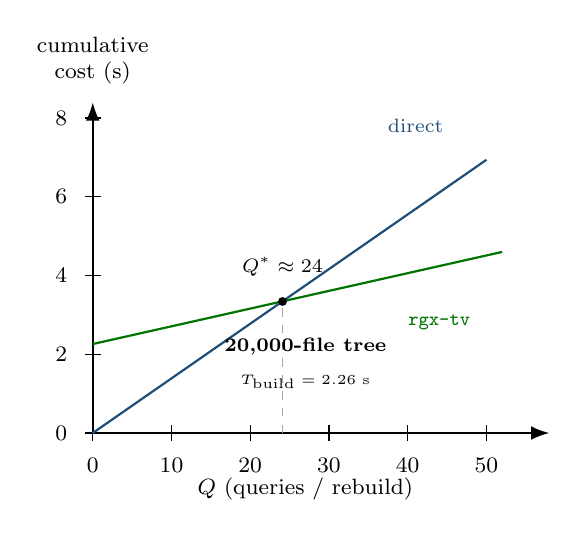
\begin{tikzpicture}[
    x=1mm, y=1mm,
    font=\footnotesize,
    >=Latex,
    axis/.style={->,thick},
    dir/.style={rgxblue,thick},
    tvp/.style={green!45!black,thick},
    lbl/.style={font=\scriptsize,align=center}
  ]
    \draw[axis] (0,0) -- (58,0);
    \node[below=4.5mm] at (27,0) {$Q$ (queries / rebuild)};
    \draw[axis] (0,0) -- (0,42) node[above=1mm,align=center] {cumulative\\ cost (s)};
    \foreach \x in {0,10,20,30,40,50} \draw (\x,1mm)--(\x,-1mm) node[below=1mm] {\x};
    \foreach \y in {0,2,4,6,8} \draw (1mm,\y*5)--(-1mm,\y*5) node[left=1mm] {\y};
    % scale: 5 coordinate units = 1 second
    % direct: C = 0.1388 Q s -> at Q=50: 6.94 s -> y = 34.7
    \draw[dir] (0,0) -- (50,34.7);
    % tv: C = 2.257 + 0.045 Q s -> at Q=50: 4.507 s -> y = 22.5; intercept y = 11.3
    \draw[tvp] (0,11.3) -- (52,23.0);
    % crossing Q* = 24.1, C = 3.345 s -> y = 16.7
    \draw[dashed,gray!70] (24.1,0) -- (24.1,16.7);
    \fill (24.1,16.7) circle (1.6pt);
    \node[lbl] at (24.1,16.7) [above=2mm] {$Q^{*}\approx 24$};
    \node[lbl,text=rgxblue] at (41,39) {direct};
    \node[lbl,text=green!45!black] at (44,14) {\texttt{rgx-tv}};
    \node[lbl,font=\scriptsize\bfseries] at (27,11) {20{,}000-file tree};
    \node[lbl,font=\tiny] at (27,6.5) {$T_{\text{build}} = 2.26$~s};
\end{tikzpicture}
\end{minipage}\hfill
\begin{minipage}[t]{0.48\textwidth}
\centering
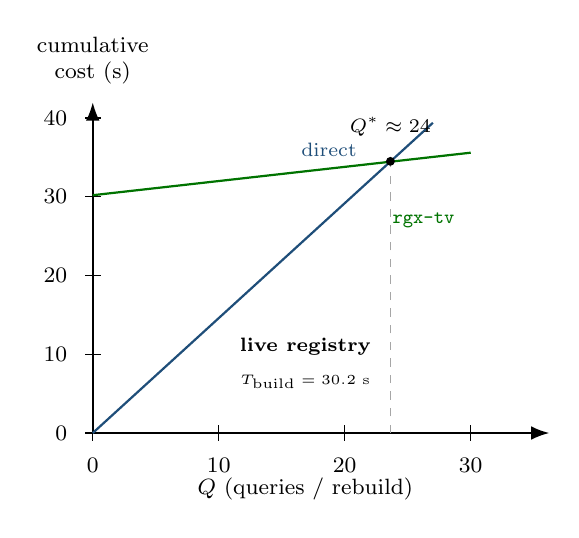
\begin{tikzpicture}[
    x=1mm, y=1mm,
    font=\footnotesize,
    >=Latex,
    axis/.style={->,thick},
    dir/.style={rgxblue,thick},
    tvp/.style={green!45!black,thick},
    lbl/.style={font=\scriptsize,align=center}
  ]
    \draw[axis] (0,0) -- (58,0);
    \node[below=4.5mm] at (27,0) {$Q$ (queries / rebuild)};
    \draw[axis] (0,0) -- (0,42) node[above=1mm,align=center] {cumulative\\ cost (s)};
    \foreach \x in {0,10,20,30} \draw (\x*1.6,1mm)--(\x*1.6,-1mm) node[below=1mm] {\x};
    \foreach \y in {0,10,20,30,40} \draw (1mm,\y)--(-1mm,\y) node[left=1mm] {\y};
    % scale: x = 1.6 coord per query; y = 1 coord per second
    % direct: C = 1.459 Q s -> at Q=27: 39.4 s -> x = 43.2
    \draw[dir] (0,0) -- (43.2,39.4);
    % tv: C = 30.22 + 0.1793 Q s -> intercept y = 30.2; at Q=30: 35.6 s
    \draw[tvp] (0,30.2) -- (48,35.6);
    % crossing Q* = 23.6, C = 34.5 s -> x = 37.8
    \draw[dashed,gray!70] (37.8,0) -- (37.8,34.5);
    \fill (37.8,34.5) circle (1.6pt);
    \node[lbl] at (37.8,34.5) [above=2mm] {$Q^{*}\approx 24$};
    \node[lbl,text=rgxblue] at (30,36) {direct};
    \node[lbl,text=green!45!black] at (42,27) {\texttt{rgx-tv}};
    \node[lbl,font=\scriptsize\bfseries] at (27,11) {live registry};
    \node[lbl,font=\tiny] at (27,6.5) {$T_{\text{build}} = 30.2$~s};
\end{tikzpicture}
\end{minipage}
\caption{The break-even phase boundary, both corpora. Left: the fixed tree.
Right: the live registry. Both axes are cumulative cost in seconds against
queries per rebuild: direct is a ray of slope $T_{\text{direct}}$,
prepared is a half-line from $(0,T_{\text{build}})$ of slope
$T_{\text{tv}}$, and the crossing is $Q^{*}$. Beyond it the gap grows
linearly in $Q$; the two corpora land on nearly the same $Q^{*}$ despite a
$13\times$ difference in build cost, because the per-query saving scales
with the same corpus size.}
\label{fig:phase}
\end{figure}

\begin{itemize}[leftmargin=*,itemsep=1pt]
\item \textbf{Direct search is preferable for $Q<Q^{*}$}: one-off ad-hoc
  terminal queries, buffers with unsaved edits, or environments with storage
  quotas that prohibit maintaining a derived pack.
\item \textbf{Prepared search is preferable for $Q>Q^{*}$}: developer
  workstations, language servers, review bots and autonomous coding agents,
  where dozens of queries run against a stable snapshot.
\end{itemize}

On the mutation axis, every invalidation cycle re-pays
$T_{\text{build}}+T_{\text{maint}}$; a corpus that mutates between every
pair of queries is the $Q\to 1$ limit and the store is pure overhead. The
shipped detector encodes the $\mu=0$ decision rule and nothing more
(\Cref{sec:limits}): it is a phase-boundary engine for the stationary
corpus, and the moving-corpus policy is left to the operator.

\paragraph{The unfavorable cases, stated at the same strength as the wins.}
Six shapes lose or tie, and each is a shape the prepared path is asked
about. A \emph{small corpus} carries a small $\sigma N$ to begin with, so
there is little metadata for packing to delete and $T_{\text{build}}$ is
never recovered. \emph{Few queries} are the $Q<Q^{*}$ side of the boundary
above. \emph{Large files} amortise the per-file cost inside the file
itself: the metadata tax is paid once per file and a file of megabytes
spends it in its own scan, so on a corpus of a few large files the direct
path is the right one. A \emph{frequently mutating corpus} and a
\emph{frequent rebuild} are the same shape seen twice: each rebuild
re-enters $T_{\text{build}}$, and at one mutation per query the store is
strictly overhead. A \emph{one-shot query} is $Q=1$ by definition --- a CI
grep over a fresh checkout is the canonical case --- and no amortisation
reaches it. None of these is an implementation gap; they are the phase
boundary of \Cref{eq:qstar} with the axes turned up.

\paragraph{Where $Q^{*}$ sits in practice.}
The measured thresholds are all in the tens of queries and are host
properties through both of their terms: $T_{\text{build}}$ (998~ms on the
second host against 2.26~s on the primary for the same 26-pack tree) and
$T_{\text{direct}}-T_{\text{tv}}$ (the per-query saving, which moves with
thread count and with which direct arm is the reference). The two hosts
bracket $Q^{*}\approx 18$--$29$ on the fixed tree; on the live registry
only the primary host ran the protocol, and its two snapshots give 23.6 and
17.3 (\Cref{sec:eval:cargo}) --- tens of queries on either corpus. For an
operator the useful form is
not a constant but the inequality: build when the expected remaining
queries on this snapshot exceed $T_{\text{build}}$ divided by the measured
per-query saving on \emph{this} machine, and do not assume a multiplier
quoted from another host. A language server that issues fifty queries
against a checkout is on the prepared side of the boundary on either
host; a one-shot CI grep is not.

\section{Where else the diode pays}
\label{sec:uses}
The phase boundary of \Cref{sec:regimes} is not a fact about
regular-expression search. It is a fact about a workload shape, and the
shape is checkable before anything is built. Three conditions are
necessary:
\begin{enumerate}[leftmargin=*,itemsep=1pt]
\item \emph{a cost per unit of structure} that does not scale with bytes ---
  the $\sigma N$ of \eqref{eq:twoterm}, and enough of it that
  $\rho=\sigma N/(B/\beta)$ is of order one or larger; below that
  \Cref{prop:separation} bounds what any transport tier can recover at all;
\item \emph{a stable corpus}: $\mu$ small enough that the build is paid
  once and read many times;
\item \emph{enough queries}: $Q$ past $Q^{*}$ of \Cref{thm:breakeven}, with
  $T_{\text{build}}$ and the per-query saving measured \emph{in the target
  domain}. Neither magnitude transfers between two hosts running the same
  code (\Cref{sec:eval:cross}), so neither is safe to quote across domains.
\end{enumerate}
What transfers is the form of the boundary and the sign of its terms; no
magnitude does. \Cref{tab:uses} therefore lists \emph{candidates} --- whose
published shape satisfies the three conditions --- and the claim in each row
is that the criterion is worth measuring there, not that a speedup has been
established.

\begin{table}[htbp]
\centering
\footnotesize
\caption{Candidate workloads, and why each one satisfies the conditions
above. $Q$ and $\mu$ are qualitative on purpose: the thresholds of
\Cref{tab:small,tab:cargo} were measured for search, and no magnitude in
this table is claimed for another domain. One row is not a candidate: the
name-search row carries a measured instance in its own domain
(\Cref{sec:uses:names}).}
\label{tab:uses}
\begin{tabular}{@{}p{0.27\linewidth}p{0.31\linewidth}p{0.30\linewidth}@{}}
\toprule
\textbf{Workload} & \textbf{The $\sigma N$ term} & \textbf{$Q$ and $\mu$} \\
\midrule
code search over a vendored dependency tree or SDK
  & traversal of $10^4$--$10^5$ small files
  & dozens of queries per edit in a language server; $\mu\approx0$ between upgrades \\
documentation and standard-library search
  & walking release artifacts
  & many readers per release; $\mu=0$ until the next one \\
log and telemetry archives
  & one pass over a partition of small records
  & a burst of queries per incident; $\mu=0$ inside the partition \\
SBOM and signature sweeps over build output
  & one traversal per scanner
  & one query per signature; $\mu=0$ for the artifact \\
reference-database lookup (an FM-index \cite{ferragina2000} over a genome, say)
  & the reference is walked once
  & one build per reference release, then queries without limit \\
retrieval over a fixed document set for a language model
  & document and chunk bookkeeping
  & one build per corpus version, many prompts \\
e-discovery and forensic keyword search
  & walking the file table of an evidence image
  & many queries per custodian request; $\mu=0$ by procedure \\
package-registry and malware-library triage
  & the registry's entry count, not its bytes
  & append-only: one build per generation, queries between ingestions \\
whole-filesystem name search (the \emph{which-file} tier)
  & enumerating the volume's directory table, $10^5$--$10^6$ entries
  & a handful of lookups per session; $\mu\approx0$ between file creations --- \textbf{measured}, \Cref{sec:uses:names} \\
\bottomrule
\end{tabular}
\end{table}

Two failures follow from the numbered conditions and are where this picture
is used carelessly. A corpus under active edit --- a mailbox, a live feed, a
working tree --- fails (2): the build is re-paid more often than it is
queried, the direct path wins, and that is the $\mu\to1$ limit of
\Cref{sec:regimes}. A corpus small in structure fails (1): when
$\rho\ll 1$ the metadata tax is not the dominant term of \eqref{eq:twoterm}
and there is nothing for the architecture to reclaim.

The rule is the same in every row of \Cref{tab:uses}, and it is not about
search: move every term that does not scale with bytes into an ingestion
pass, and keep the hot path a table walk. Measure $\rho$ first --- it is the
one number that says how much is there to reclaim, and
\Cref{prop:separation} turns it into a ceiling on both tiers at once via
\eqref{eq:smax} ($1+\rho^{-1}$ for a perfect matcher, $1+\rho$ for a perfect
transport tier). Three of the rows now have a measurement behind them, the third being
the name tier of \Cref{sec:uses:names}, where no regular expression is
involved at all. The
$\mu=0$ assumption is weaker than it looks. Under the steady-state
instantiation of \Cref{thm:breakeven} --- build sunk, each invalidation
cycle paying the refresh alone --- a 1\% mutation of the fixed tree prices
its refresh at 626.2~ms against a 65.4~ms per-query saving (\texttt{fn
main}, \texttt{-j32}), $Q^{*} = 626.2/65.4 \approx 9.6$ queries per cycle,
and a 10\% mutation prices its refresh at 887.6~ms against 64.9~ms,
$Q^{*} \approx 13.7$ (\path{benchmark/mutation-transcript.md}) --- the
maintenance loop keeps the boundary in the tens of queries under growth,
which is what the append-only rows lean on. And the file-size direction of
the first condition is visible:
on a generated log partition (5{,}000 files, 221~MB, median 44~KB) the
store's margin over ripgrep is 1.5--1.6$\times$, against 2.3--2.5$\times$
on the many-small-files tree under the same four-arm harness
(\path{benchmark/log-corpus-transcript.md},
\path{benchmark/ugrep-transcript.md})
--- $\rho$ moving the wrong way as files grow, exactly as the condition
predicts. The valvular conduit is a shape, not a product.

\subsection{Name search at filesystem scale}
\label{sec:uses:names}
The \emph{which-file} tier of \Cref{tab:uses} is the one row whose
$\sigma N$ term no search engine owns: a name lookup over a volume pays
it by enumerating the directory table, and no regular expression is
involved at all. The three conditions of \Cref{sec:uses} hold by
construction --- the structure is the entry count, the tree is a
filesystem between file creations, and a session asks a handful of
lookups --- so this row carries a measured instance in its own domain
rather than a place in the candidate list.

The instance is the rgy name tier under the protocol of \Cref{sec:eval},
on the primary host: the direct arm enumerates the tree and matches
names --- what \texttt{fd} and \texttt{dir /s} do, no index built --- and
the indexed arm answers from a name index persisted at build time and
pays its load \emph{inside} the timed invocation, setup charged rather
than hidden. Corpora of 200{,}000 and 5{,}000{,}000 entries are
materialized as real files --- the second past the $10^5$--$10^6$ range
of \Cref{tab:uses}, which is the conservative direction, since a larger
table raises the walk arm's $\sigma N$ and lowers $Q^{*}$ --- and at both
scales every indexed minimum is below the corresponding walk minimum, so the
table names the same winner on every row at both scales (\Cref{tab:names}).
Only that ordering of minima is claimed. The per-round distributions that would
separate the two arms in the sense \Cref{sec:predictions} uses are not part of
this deposit, so separation is not claimed from these rows.

\begin{table}[htbp]
\centering
\footnotesize
\caption{Name search at the \emph{which-file} tier, on the primary host of
\Cref{sec:eval}. The direct arm enumerates the directory table and matches
names; the indexed arm answers from the persisted name index and pays its
load \emph{inside} the timed invocation. Minima of seven paired rounds with
arm order rotated, a count gate in front of every timing line. Every retained
row has a lower minimum latency in the indexed arm; distributional separation
is not established by the summary statistics reported here, and the per-round
samples behind these minima do not accompany this deposit. $Q^{*} =
\lceil T_{\text{build}} / (T_{\text{walk}} - T_{\text{query}}) \rceil$ is
\Cref{thm:breakeven}'s crossing, computed from these minima.}
\label{tab:names}
\begin{tabular}{@{}lrrrr@{}}
\toprule
\multicolumn{5}{@{}l}{\emph{200{,}000 entries materialized} --- build 85.5~ms (min of 7), process floor 13.88~ms} \\
\midrule
query & walk min (ms) & index min (ms) & ratio & $Q^{*}$ \\
\texttt{report} & 47.6 & 21.46 & 2.2$\times$ & 4 \\
\texttt{file} & 46.0 & 24.19 & 1.9$\times$ & 4 \\
\texttt{'report\_00000.pdf} & 45.1 & 17.51 & 2.6$\times$ & 4 \\
\texttt{\^{}src} & 45.3 & 21.02 & 2.2$\times$ & 4 \\
\texttt{dat\$} & 45.1 & 23.76 & 1.9$\times$ & 5 \\
\texttt{mod} & 47.5 & 23.70 & 2.0$\times$ & 4 \\
\texttt{rep} & 46.9 & 20.90 & 2.2$\times$ & 4 \\
\midrule
\multicolumn{5}{@{}l}{\emph{5{,}000{,}000 entries materialized} --- build 2{,}221.1~ms (min of 7), process floor 12.01~ms} \\
\midrule
query & walk min (ms) & index min (ms) & ratio & $Q^{*}$ \\
\texttt{report} & 604.6 & 91.49 & 6.6$\times$ & 5 \\
\texttt{file} & 586.1 & 134.52 & 4.4$\times$ & 5 \\
\texttt{'report\_00000.pdf} & 570.7 & 69.45 & 8.2$\times$ & 5 \\
\texttt{\^{}src} & 565.9 & 110.80 & 5.1$\times$ & 5 \\
\texttt{dat\$} & 560.1 & 136.12 & 4.1$\times$ & 6 \\
\texttt{mod} & 613.1 & 108.57 & 5.6$\times$ & 5 \\
\texttt{rep} & 614.1 & 91.62 & 6.7$\times$ & 5 \\
\bottomrule
\end{tabular}
\end{table}

The boundary is \Cref{thm:breakeven}'s crossing in this domain, $Q^{*} =
\lceil T_{\text{build}} / (T_{\text{walk}} - T_{\text{query}}) \rceil$
from the same minima, and it lands at four to five lookups at 200{,}000
entries (85.5~ms of build against a 21.3--27.6~ms saving per lookup) and
five to six at 5{,}000{,}000 (2{,}221~ms against 424--522~ms). A handful
of lookups per session --- the shape \Cref{tab:uses} already claims ---
is past that boundary on both corpora. The ratio column moves from
1.9--2.6$\times$ to 4.1--8.2$\times$ as the table grows, which is the
first condition of \Cref{sec:uses} visible: the walk arm's cost is the
entry count, the indexed arm's is the match set plus one load.

One query of the eight is suppressed by the count gate at both scales and
is not timed: \texttt{f1}, the fuzzy form, which the direct arm does not
implement --- it answers 0 where the index answers 80{,}547 and
1{,}639{,}704 entries. That disagreement is what the gate exists to
catch, and the row's absence is its honest outcome. The claim in
\Cref{tab:claims} is falsified by a name workload where the indexed arm
loses past its own break-even count; nothing in this grid moves that way.
Two directions of conservatism bound what the table says: the walk arm
scans with sixteen threads where the indexed arm uses its own runtime
parallelism, and the timer is the wall clock around the whole process ---
the in-process illusion of \Cref{sec:mmap} is exactly what this protocol
refuses to price out.

\section{Ablations: what each tier contributes, and what is not isolated}
\label{sec:ablations}
A headline ratio is a property of the stack, and a paper that attributes
it to a tier without an ablation is reading a component measurement into
an end-to-end one. \Cref{tab:ablation} is the accounting: which
single-tier effects are measured on their own, which end-to-end ablations
exist, and which do not.

Three tiers have component-level evidence and one comparison is
end-to-end. The transport tier is isolated by the zero-match row of
\Cref{tab:cargo} --- 220~ms of pack read against 1{,}465~ms of direct
search over the same 1.94~GB; the mask by the scalar reference of
\Cref{tab:dio}, which counts candidates quenched per shape before any
confirmation; the signature by the standalone harness of
\Cref{tab:ngram}, which counts files pruned per pattern. The end-to-end
evidence is the store against the direct arms of \Cref{sec:eval}, and it
measures the stack.

The two tiers now have end-to-end ablations, run through query-path
switches built for the purpose --- \texttt{RGX\_ABLATE\_MASK} declines the
compiled mask at pattern compile, \texttt{RGX\_ABLATE\_NGRAM} forces the
signature's stand-down state --- under the same count gate and the same
min-of-seven protocol. Both switches change cost and never answers: the 36
arm comparisons across the nine patterns agreed on every summed count, and
the vacuity checks show each switch did something (the mask anchor
disappears from the pattern's anchor list; the store's
\texttt{files\_pruned} counter falls from 6{,}049 to 0 of 20{,}000). The
gate earned its keep on the first run, which refused a row whose store arm
silently matched nothing: its argument parser read a pattern containing
\texttt{=} as a bundled option --- a defect the run found and the
binary's tests now pin.

The result has two shapes. The \emph{mask} is end-to-end visible where
declining it forces a substantially more expensive fallback stage: on the
registry corpus declining it costs \textbf{+46\%} on
\texttt{(pub|fn) [a-z]+} (173 to 253~ms) and $+8.6\%$ on \texttt{a|b}
(186 to 202~ms), and on the single-file \texttt{big235.rs} corpus of
\Cref{tab:dio} (\texttt{-j1}, 7 paired rounds rotated,
\path{benchmark/findings.md}~\S 19) it separates on three of the nine
shapes --- \textbf{+109.6\%} on \texttt{(pub|fn) [a-z]+} (148.1~ms
$[144.8\dots 152.6]$ to 310.4~ms $[307.8\dots 316.0]$, 1{,}236{,}465 lines),
\textbf{+49.6\%} on \texttt{e.} (187.3~ms $[181.5\dots 188.4]$ to 280.3~ms
$[274.0\dots 284.6]$, 6{,}927{,}072 lines) and \textbf{+23.5\%} on
\texttt{a|b} (171.4~ms $[165.0\dots 180.3]$ to 211.7~ms $[208.0\dots 222.4]$,
5{,}269{,}846 lines) --- while \texttt{e[0-9]} (240{,}786 lines, 98.51\%
quenched in \Cref{tab:dio}) moves by $+7.6\%$ (75.3~ms $[74.2\dots 80.2]$
to 81.0~ms $[77.6\dots 85.9]$), which the range gate refuses as
\emph{overlap, not a result}, and the five pure-literal and line-window rows
sit inside the $\pm 3\%$ floor ($-1.5\%$ to $+1.0\%$). That ordering is why
candidate-stream diodicity (\Cref{tab:dio}) is a placement metric rather than
a wall-clock speedup predictor: end-to-end wall-clock cost under
\texttt{RGX\_ABLATE\_MASK=1} is governed by which fallback stage catches the
stream when the mask is declined (\texttt{(pub|fn) [a-z]+} loses its
\texttt{premask} and has no single literal prefix for \texttt{memchr} to
fall back to; \texttt{e.} and \texttt{a|b} drop from single-pass
\texttt{matchmask} line settlement to per-candidate confirmation over
millions of lines; \texttt{e[0-9]} falls back to \texttt{memchr('e')} plus a
one-byte digit check against a $\approx 65$~ms process/I/O floor), which is
the complementarity of \Cref{prop:separation} appearing inside one tier's own
fallbacks. The \emph{signature} is inside the floor everywhere (at most
2~ms on a 140--210~ms query, $\le 1\%$) even where it prunes 30\% of the
files, and the in-process breakdown names the reason: a pruned file's
bytes are read at pack granularity regardless, so the filter saves scan
and confirm work (the regex leg moves 49 to 54~ms of CPU) and no read work
(135~ms of CPU, the dominant leg). The signature is worth its 2--7~ns per
file and is not a wall-clock lever at this scale --- which is what
``component measurement, not end-to-end claim'' meant when this ledger had
two empty rows. Both effects replicate on the second host, where the
mask's absence costs more still (\texttt{(pub|fn) [a-z]+} 64 to 98~ms,
$+53\%$; \texttt{a|b} $+19\%$) and the signature again sits inside the
floor (\path{benchmark/ablation-transcript-linux.md}).

\begin{table}[htbp]
\centering
\footnotesize
\caption{The ablation ledger. ``Component'' is a measurement of the tier
in isolation; ``end-to-end'' is the same query with the tier on and off.
A row is a claim about the tier's contribution only when the second
column is filled.}
\label{tab:ablation}
\begin{tabular}{@{}>{\raggedright\arraybackslash}p{0.19\linewidth}>{\raggedright\arraybackslash}p{0.31\linewidth}>{\raggedright\arraybackslash}p{0.25\linewidth}>{\raggedright\arraybackslash}p{0.13\linewidth}@{}}
\toprule
\textbf{Tier} & \textbf{Component evidence} & \textbf{End-to-end ablation}
  & \textbf{Status} \\
\midrule
transport (pack against per-file)
  & zero-match row of \Cref{tab:cargo} (220~ms against 1{,}465~ms)
  & store against direct arms (\Cref{tab:small,tab:cargo,tab:linux})
  & measured \\
mask (OR of ANDs)
  & scalar reference of \Cref{tab:dio} (candidates quenched)
  & same query with the mask declined at compile
  & measured: $+46\%$ / $+8.6\%$ on registry; $+109.6\%$ (\texttt{(pub|fn) [a-z]+}), $+49.6\%$ (\texttt{e.}), $+23.5\%$ (\texttt{a|b}) on \texttt{big235.rs} \\
n-gram signature
  & standalone harness of \Cref{tab:ngram} (files pruned)
  & same query with the filter stood down
  & measured: inside the floor ($\le 1\%$) \\
\bottomrule
\end{tabular}
\end{table}

\section{Threats to validity}
\label{sec:limits}

\paragraph{The analogy is bounded, and the bound is stated.}
The storage tier is an architectural inspiration, not a physical model: bytes
do not flow, and \Cref{rem:nse} shows why the queueing layer needs its own
theory. The microarchitectural tier is a genuine functional analogue, but its
mechanism is an OR of ANDs over combined byte classes, not a
forward-against-reverse collision; we state this in \Cref{sec:micro:shape}
precisely because the more evocative description is wrong about the code.

\paragraph{Diodicity is defined twice, differently.}
The candidate-suppression ratio of \Cref{sec:dio} is
$\text{naive}/\text{admitted}$. The project's own diodicity harness
operationalises the term as \emph{blocked-side work divided by performed
work}, and under that stricter definition it identifies the pack store
itself as a \emph{negative control} --- a pipe, not a valve --- because a
prepared store makes the reverse direction cheaper rather than forbidden.
Both are defensible definitions; they are not the same claim, and a reader
should not carry one into the other.

\paragraph{The mask ratios are properties of the mask, not of the loop.}
\Cref{tab:dio} is produced by a scalar reference evaluation of the compiled
predicate. The production AVX2 kernel computes the same predicate set, and
the false-negative guarantee rests on \Cref{thm:fnr} and on a differential
suite, not on that table.

\paragraph{The 512-bit ``inversion'' was a reporting error, not a finding.}
A mislabelled transcription of the n-gram harness output had 512-bit
admitting more files than 256-bit, contradicting the idealised Bloom
prediction, and its apparent inversion was taken as an open doubt with a
candidate mechanism. The harness prints admitted, pruned, and
prune-efficiency columns; the transcription copied the
pruned count and the prune efficiency into a column labelled ``admitted''.
Both runs, once labelled correctly, show 512-bit pruning strictly more
files on every pattern, which is the textbook direction
(\Cref{sec:ngram:inversion}). No mechanism is claimed for the non-event.
What remains narrower and stated: the prune rates are the standalone
harness's, over one digest-named corpus in one timer scope on both hosts
(\Cref{sec:ngram}); the filter ships on the query path with the same
signatures. \Cref{sec:ablations} evaluates it end to end and finds no
wall-clock improvement above the floor, which is a different statement from
having not measured it.

\paragraph{The streaming advantage is regime- and cell-bound.}
In \Cref{tab:nine}, \texttt{ParallelBuffered} beats \texttt{mmap} by
$-43.5\%$ to $-67.3\%$ on scan-bound count rows and by $-9.8\%$ to $-11.2\%$
on the output-bound full-output row (8 of 9 cells separated on the
93{,}234-file, 114-pack corpus; \texttt{pub fn} count at $-j1$ overlapped);
the same comparison on the smaller 20{,}000-file corpus overlapped on this
host, while the second host of \Cref{sec:eval:cross} finds
\texttt{ParallelBuffered} faster than mmap by 3--18\% (mean $\approx 12\%$)
on that 20{,}000-file corpus. The \emph{direction} --- buffered beats mmap
on a one-shot query --- is observed on two hosts and two corpora; the
\emph{magnitude} depends on whether the query is scan-bound or output-bound
and on corpus size. What is robust is the qualitative mechanism (page-fault
integral plus deferred teardown, \Cref{tab:unmap}), not a single constant.

\paragraph{Cross-session ratios drift more than the floor.}
Absolute milliseconds on this machine move by tens of per cent across
sessions; the project harnesses treat $\pm 3\%$ as the no-result floor for a
single paired run. Two runs of the same pack-store protocol on the same
tree corpus, one day apart, produced 6.13--6.55$\times$ against ripgrep
(2026-10-10) and 2.79--3.38$\times$ (2026-10-11, \Cref{tab:small}); the
2026-10-10 ripgrep arm is the outlier against every other measurement of
that corpus on this machine (120--150~ms), while the 2026-10-11 arms agree
with them. We publish the paired run whose \emph{reference arm} sits inside
the established band and treat the other as evidence that this harness's
minimum-of-$N$ estimator, lacking the distribution gate of the main
dashboard, admits more between-session variance than a single run shows.
Ratios quoted without their run date and reference-arm placement should not
be compared across papers.

\paragraph{The headline ratio is regime-dependent.}
The pack store streams sequentially and is matched against a
thread-parallel direct search. The ratio therefore moves with the thread
count granted to the direct engine, and it also moves with corpus shape:
a comparison at another thread count, or against a store invalidated
between queries, is a different experiment. The two corpora here sit at
different $N$, different $\rho$, and different thread counts by design.

\paragraph{The live-registry multiplier was measured on a store arm that did
not run the full pipeline.}
\Cref{tab:cargo} reports store-versus-ripgrep ratios whose parity holds
because the store arm of that snapshot did not surface container text, not
because the store is defined to agree with ripgrep. The construction's parity
is store-with-direct (\Cref{thm:equivalence}); on the two patterns where the
direct arm exceeds ripgrep by a non-zero count, a store built to run the full
pipeline would exceed ripgrep by the same amount, and no ratio against ripgrep
would be a ratio between the same two searches. The two affected ratios are
therefore properties of a reduced build, marked $\dagger$ and excluded from
the reported range, and this paper does not report the full-pipeline number for
that corpus. The retained range remains a valid measurement of the historical
configuration, but it does not establish the performance of the full
container-extraction pipeline: the two endpoints of the range, $6.66\times$ and
$12.41\times$, are both from rows whose store
view coincides with ripgrep's, as are the two $\beta_{\text{pack}}$ and
matcher-ceiling results quoted beside it. The cross-host pack-store protocol is
unaffected --- it runs on the fixed 20{,}000-file corpus, where all three arms
are exact count parity on every row (\Cref{tab:linux}).

\paragraph{Two hosts, not one; still not a population.}
The primary numbers are one Windows host. A second host (Linux,
Ryzen~7~255) has re-run the pack-store protocol, the read-mode probe and
the n-gram harness on identical corpora (\Cref{sec:eval:cross}); the
architecture claim and the read-mode direction transfer, the headline
multipliers and the matcher margins do not. Two hosts are enough to show
that a ratio is not a constant of the code and not enough to characterise
the distribution of that ratio. The page-fault argument of
\Cref{sec:mmap} is Windows-specific in its syscall accounting; the pack
store's advantage still depends on the corpus being a large set of small
files, and on a few large files the direct path is the right one --- there
the metadata tax is not the dominant term of \eqref{eq:twoterm} and an
architecture has nothing to reclaim. The transport share $s_{\text{I/O}}$ of
\Cref{lem:amdahl} comes from the zero-match reading of one row of
\Cref{tab:cargo}, not from an instrumented split, and should not be
assumed elsewhere.

\paragraph{Generality of the engine, not just of the numbers.}
The matcher is a byte-mode engine at scan and confirm time. Simple Unicode
case folding is resolved at parse time (\path{unicode\_case.rs}): under
\texttt{(?i)} or \texttt{-i}, each character expands into the byte
alternation of its simple case-folding equivalence class (mixed UTF-8 widths
included) and literal extraction declines any caseless literal whose class
leaves ASCII (\texttt{k} and \texttt{s}), so \texttt{-i kelvin} matches
U+212A KELVIN SIGN and \texttt{(?i)\ss} matches U+1E9E~\texttt{\SS}. The
remaining Unicode limits are structural: a multi-byte codepoint inside a
bracketed character class is split into byte ranges (so \texttt{[\'e]} in a
mixed class over-matches), full multi-character case mappings are not
expanded (\texttt{\ss} does not match \texttt{SS}), and conditional
final-sigma folding is not applied. A pattern outside the accepted grammar
(such as lookaround or backreferences) is refused at parse time rather than
matched approximately, so the grammar boundary is visible at the command
line and never a silent difference between two engines.
Every timing in this paper ran a vector fill of the shipped binary, chosen
by its host: the primary host's Zen~4 core exposes AVX-512BW and ran that
fill, while the AVX2 fill of \Cref{code:kernel} is the portable vector
path. The scalar fill is the definition the vector fills implement and is
tested against them, but no timing here measures it in isolation; the
claims attach to the predicate set, which every fill computes identically
(\Cref{prop:cover} is the construction, and the fills are pinned against
the scalar definition by a differential suite).

\paragraph{The corpora are code-centric.}
Both measured corpora are software repositories (a generated Rust tree and
the live Cargo registry) and the n-gram corpus is 15{,}000 \texttt{.rs}
files. Log partitions are not: a generated 5{,}000-file partition is measured and
reports where the advantage narrows
(\path{benchmark/log-corpus-transcript.md}), so that row is a boundary and not
a candidate. Natural-language documents, mail stores and binary
payloads are unmeasured here, so every row of \Cref{tab:uses} outside code
and log search is a candidate and not a result. What both corpora do carry is the
shape the metadata tax needs --- many files, median 4.4~KiB --- and a
domain whose files are larger or fewer moves $\rho$ the wrong way
(\Cref{sec:uses}).

\paragraph{The store duplicates its corpus, in plaintext.}
A pack holds file bytes verbatim --- which is what makes
\Cref{thm:equivalence} cheap --- and the consequence is operational: the
corpus exists twice, at roughly its own size plus the manifest; there is no
deduplication and no encryption at rest; removing one file's content from
the world means rebuilding or rewriting the packs that hold it, because a
slice is not a reference but a copy; and a store on shared storage exposes
everything the corpus contains. These are properties of the design and not
defects, and they bound the workloads of \Cref{sec:uses} where retention
policy matters --- the e-discovery row of \Cref{tab:uses} is where this
bites hardest.

\paragraph{Crash consistency is a protocol claim, not a measurement.}
The publish path is write, \texttt{fsync}, rename, with packs flushed
before the manifest that names them, so a reader observes generation $G$ or
$G{+}1$ whole. Two assumptions sit under ``whole'': the rename is atomic at
the filesystem --- on Windows, the primary host, a replace-existing move
whose guarantee is the filesystem's and its filter drivers', weaker than
the POSIX rename the construction invokes --- and the packs of generation
$G$ remain reachable while $G{+}1$ is written, which is what keeps a
mid-rebuild reader off torn payloads and what the free-space cost below
pays for. What is not measured is recovery: the behaviour of a pack
torn by a crash mid-write, the time to detect and rebuild a store after
one, and the free-space cost of keeping both generations reachable. The
protocol is the standard atomic-publish construction; its crash behaviour
is asserted from that construction and not tested here. A pack whose bytes
rot after publication is caught by \texttt{inspect}, not by the query
path, which trusts the manifest and the lengths it records.

\paragraph{A binary verdict that is not the searchers' rule fails in the
wrong direction.}
The store's \texttt{is\_binary} bit is the searchers' own classification ---
whole content, byte-order mark decoded first --- computed once at build, and
the direct path applies the same rule at query time, so store and direct
decide alike at different moments (\Cref{tab:boundary}). Any proxy verdict
(an initial-buffer sniff, a raw-NUL test on a marked file) classifies
late-NUL or UTF-16 content differently, and the failure lands as
\emph{extra} matches on one arm --- visible to a count gate that demands
equality, invisible to one that only checks nothing was lost. Cross-engine
the same boundary applies: ripgrep's verdict lives inside its searcher, so
store-vs-ripgrep parity is the count gate's empirical claim, not a
consequence of \Cref{thm:equivalence}.

\paragraph{The format is a compatibility commitment.}
The manifest carries a version, and a store of any other version is refused
with its version named --- parsed on a guess would be worse --- which makes
format evolution a rebuild rather than a migration, and long-lived stores a
build-version dependency. The layout of \Cref{tab:format} is asserted on
read, so drift is loud rather than silent; what is not measured is the cost
of carrying old stores forward, because the format has not yet had to move.

\paragraph{The end-to-end numbers measure the stack, and so do the
ablations, narrowly.}
The end-to-end comparisons measure the stack under the configuration
recorded for each run. The live-registry store arm of \Cref{tab:cargo} did not
surface container text, and its two affected patterns are excluded from
performance ratios and from aggregate break-even calculations. The fixed-corpus
comparisons and the cross-host replication retain exact count parity across all
three arms. The two filtering tiers now have ablations
(\Cref{sec:ablations}), and they show exactly two end-to-end effects: the
mask, on patterns with no fallback anchor; the signature, none above the
floor. What remains unmeasured is the transport tier's separate share of
the headline ratio --- the store's win is the stack's, and ablating
``manifest and pack read'' is the store-versus-direct comparison itself
--- and the overlap between the two filtering effects. Attributing a
share of the headline ratio to any one tier beyond what
\Cref{sec:ablations} measures would be reading a component measurement
into an end-to-end one.

\paragraph{What the evidence bounds.}
The sparse-pair row of \Cref{tab:dio} sits at its measured ceiling ---
50.00\% quenched, and the 264{,}029 candidates it admits are exactly the
matches --- so anchoring its second literal at any distance leaves that
number unmoved on this corpus. The detector's freshness gate answers
\emph{changed} files and names the snapshot it declined; a file added
after the build is the one shape it cannot see without the walk the store
exists to avoid, and \texttt{--tv-build} is the refresh.

\section{The diode as a design instrument: finding the prefilter}
\label{sec:calculus}
\paragraph{What the residue is for.}
\Cref{sec:demarcation} leaves the fluid picture with a residue: design
discipline and vocabulary, and no prediction. This section makes the
residue operational. The design question it answers is the one every
pipeline with a cheap first stage must answer anyway: \emph{given a
pattern and a candidate stream, find the prefilter} --- the stage that
refuses as many false candidates as possible per unit cost and refuses no
true match. The valve supplies the objective and the vocabulary; the
asymmetric-work organisation of \Cref{sec:theory} and the compile-time
obligation of \Cref{thm:fnr} supply the constraints; the output is a
design, not a speed.

\subsection{The design problem in the valve's terms}
\label{sec:calculus:terms}
The flow is the naive candidate stream $C_0$ of \Cref{def:candidates}: one
packet per offset of the chosen high-frequency prefix. The forward
direction is a true match, the reverse direction a false candidate.
Forward resistance must be exactly zero --- $\mathrm{FNR}=0$ is perfect
forward conductivity, and the hypothesis of \Cref{thm:fnr} (every term a
necessary condition of its own alternative at its own offset) is the
engineering form of that specification: a term with any forward drop is
not a vane, it is a leak. Reverse resistance is the only free variable,
and the figure of merit is the diodicity of \eqref{eq:di}, which at this
tier is not a metaphor but a count --- candidates refused per candidate
admitted, the quenched column of \Cref{tab:dio}. \emph{Finding the
prefilter} therefore means: choose and arrange the terms so that reverse
resistance per broadcast is as large as the pattern allows.

\subsection{The calculus: five questions}
\label{sec:calculus:questions}
\begin{enumerate}[leftmargin=*,itemsep=1pt,topsep=2pt]
\item \textbf{What flows?} Measure the naive stream before choosing
  anything: candidates per byte at the inlet. A dense prefix is high flow
  and the valve has work to do; a sparse prefix is already clean and the
  valve is a straight pipe --- the operating ceiling the sparse row of
  \Cref{tab:dio} sits at. Flow first, geometry second.
\item \textbf{Which vanes?} A term may enter only if it is a
  \emph{necessary} condition for a match of its own alternative at its own
  offset --- the zero-forward-drop specification, discharged at compile
  time. Among admissible terms the vane's angle is its selectivity per
  broadcast: how often the class fails on a false candidate, divided by
  the vector work it costs. The plate geometry is the class compilation of
  \Cref{sec:foundations:cover}: the nibble-grid rectangle cover is how one
  vane is manufactured out of membership tables.
\item \textbf{In what order?} Terms run as a cascade ordered by refusal
  per cost, and the block leaves the valve as soon as one conjunction
  fails --- the early-out of \Cref{code:mask} is the bypass, and the
  canonical grouping there is parallel plates: one broadcast, many
  candidate offsets.
\item \textbf{What throat?} The narrowest branch window $w$ is the
  throat. \Cref{cor:width} is the geometry --- a match of width $m$
  occupies exactly $m$ bytes --- and the window-fit rule of
  \Cref{sec:foundations:abs} settles a line from the bitmap alone exactly
  when a bit survives inside $[s,e-w]$. Sizing $w$ decides which lines the
  valve settles and which fall through to the automaton;
  \Cref{thm:window} is the machine-checked reason the byte engine's word
  is final on an ASCII window.
\item \textbf{What screen upstream?} When the unit of flow is a file, the
  inlet takes a coarse sieve before any slice is borrowed: the 512-bit
  n-gram signature of \Cref{sec:ngram} refuses whole files under its own
  soundness contract, and a screen is the cheapest vane there is --- it
  refuses at the granularity of the corpus, not of the byte.
\end{enumerate}

\subsection{The worked derivation: the shipped prefilter}
\label{sec:calculus:worked}
The five questions find the shipped design with no free parameter left
over. Question~1 chose the high-frequency literal as the inlet because
its stream is dense on the corpora the search targets; the scan is
\path{crates/rgx-core/src/prefilter.rs} and it produces $C_0$ and nothing
else. Question~2 is the mask compiler's admission rule --- only terms a
compile-time check proves necessary survive (\Cref{sec:foundations:abs})
--- over the 256-bit membership tables of
\path{crates/rgx-core/src/byteclass.rs}, with the nibble-grid cover of
\Cref{sec:foundations:cover} as the geometry that turns tables into
broadcasts. Question~3 is the order and grouping of \Cref{code:mask}:
cheap terms first, early-out on the first failing conjunction, identical
branch patterns canonicalised so one broadcast feeds many offsets.
Question~4 is the line-cut of \Cref{sec:foundations:abs} with $w$ the
narrowest branch window, backed by \Cref{cor:width} and
\Cref{thm:window}. Question~5 is the n-gram signature, a second filter
distinct in kind (\Cref{sec:ngram}). Where the picture and the code
disagree, the code is the claim; what the calculus adds is that every
part has a question that produced it, so a change to the design has a
place to be argued from.

\subsection{A second application: the rule-set scanner}
\label{sec:calculus:second}
Take a workload of the \Cref{tab:uses} shape that has no prefilter yet:
many small files, a stable corpus, queries past the break-even count, and
a rule set where each rule carries its own literals and classes --- a
signature scanner over a document archive, for instance. The same five
questions produce the arrangement directly. The inlet is each rule's
rarest literal and the flow is measured per rule, because a rule set is a
bank of valves sharing one pipe. Each rule admits only its own necessary
terms, so no rule's vane can drop another rule's match ---
\Cref{thm:fnr} applies branchwise. The cascade orders each rule's terms
by that rule's selectivity per broadcast, and the bank runs its rules in
the order of their inlet selectivity, so the cheapest refusals happen
first. Each rule's throat is its own $w$, and a line shorter than the
widest rule's throat falls through to confirmation. One shared
file-level screen is the union of the rules' signatures --- the inlet
sieve at the granularity the corpus is stored at. The output is a
concrete design. What it claims is the criterion of \Cref{tab:uses} ---
worth measuring in the target domain --- and where its suppression will
concentrate: on the rules whose secondary constraints are selective,
which is the suppression row of \Cref{tab:claims} and the measurement
protocol of \Cref{tab:dio}.

\subsection{A third application: the store, the pool, and the caps}
\label{sec:calculus:third}
The same five questions organise three layers the engine already has,
and every answer is a placement with a falsifier, not a prediction.

\textbf{The pack store} (\Cref{sec:storage}). What flows is the
per-query candidate set of files. The vanes are the per-file $512$-bit
n-gram signatures (\Cref{sec:ngram}): the query signature is built from
the literal every match must contain and stands down to searching
everything when the pattern offers no such literal, so the screen is a
necessary condition and drops nothing --- the store answers exactly as
isolated file search would, by \Cref{thm:equivalence}. The order puts
the signature before any pack slice is borrowed; the throat is the
per-file slice; the screen upstream is the manifest, one signature per
file at the granularity the corpus is stored at. The asymmetry the
valve supplies here is the generation boundary: forward is a query,
reverse is a mutation, and a mutation re-pays the build, which is what
\Cref{thm:breakeven} amortises. The freshness gate is the reverse-leak
detector --- a store the filesystem disagrees with declines to the
direct path rather than answer from bytes that no longer exist.
Falsifier: a query answered differently by the store and the direct
path, or a stale store promoted past its manifest. Under a store built
over \path{crates/rgx-core/src} (103 records) and \path{crates} (525
non-adapter records; \path{benchmark/findings.md}~\S 19), a pattern with
no required four-byte literal (\texttt{e[0-9]}) stands down as specified
(0 files pruned in both arms, 331 and 1{,}721 matches), while four-byte
literal patterns prune in the base arm (\texttt{pub fn} 10/103 and
82/525; \texttt{fn main} 12/103 and 91/525; \texttt{ByteRegex} 11/103
and 85/525; \texttt{let mut} 9/103 and 85/525) and prune 0 under
\texttt{RGX\_ABLATE\_NGRAM=1}, with identical match counts (835/1{,}143,
15/150, 145/189, 1{,}586/3{,}797) across direct search, the base store,
and the ablated store (\path{tests/ablation.rs}).

\textbf{The worker pool}. What flows is work per worker, and here the
fluid picture stops: a pool is a queue, governed by Little's law
(\Cref{rem:littl}), and the modelling boundary of \Cref{rem:nse}
forbids continuum equations from predicting queue dynamics. What the
valve retains is the one-way intake: a file admitted is a file
finished, the size and member budgets are relief at the inlet, and a
candidate refused early never enters the expensive stage. The
demarcation splits inside one layer --- queueing arithmetic is a model
because it computes; the valve vocabulary is inspiration. Falsifier: an
admitted file dropped before completion, or a queue that grows without
the relief the budgets are said to provide.

\textbf{The caps} (\texttt{OutputCap}, the member budgets of
\texttt{compress/cap.rs} and the archive budget). What flows is decoded
bytes. The cap is a threshold device with a declared breakdown: below
the limit the decode passes at full fidelity, at the limit the read
stops and is reported as \texttt{capped} beside the file's own bytes,
so a short read never masquerades as a whole one. The regime change is
observable and named --- the truncation note is itself searchable ---
and the threshold vocabulary here is the diode's, demarcated as
inspiration: no equation computes the boundary. Falsifier: a capped
read whose boundary is not where the cap declares it, or a truncated
payload returned without the note. On
\path{crates/rgx-core/testdata/zip_text_deflate.zip} (two members,
\texttt{readme.txt} and \texttt{nested/inner.bin}, each with
\texttt{declared\_size = 1{,}140}~bytes, checked by
\texttt{MemberSink::fits} in
\path{crates/rgx-adapters-archive/src/budget.rs}), sweeping
\texttt{RGX\_MAX\_MEMBER\_BYTES} pinpoints the step transitions to the
single byte: $\le 1{,}139$~B extracts $0\text{ of }2$ members and emits
the searchable \texttt{[rgx: archive truncated: 0 of 2 members extracted
(\dots)]} note (1 match for \texttt{-c "a"}); $1{,}140\dots 2{,}279$~B
extracts $1\text{ of }2$ members (60 matches in \texttt{readme.txt} plus
1 in the truncation note); and $\ge 2{,}280$~B extracts both members in
full ($60 + 60$ matches, no truncation note).

None of the three placements above carries a number the physics
supplied; each is checkable by the measurement protocols fixed in
\Cref{sec:eval} and \Cref{tab:dio}.

\subsection{What the calculus does not do}
\label{sec:calculus:limits}
The direction of explanation of \Cref{sec:demarcation} is unchanged. The
engine of the derivation is the asymmetric-work organisation and the
compile-time necessity check; the fluid picture is the vocabulary the
procedure is written in and the origin of its objective. No equation here
computes a latency: the speedup remains the measured claim of
\Cref{sec:eval}, and the phase boundary of \Cref{sec:regimes} decides
when the architecture is worth building at all. What the calculus
predicts is placement --- where a filter's suppression concentrates ---
and its falsifier is the one \Cref{tab:claims} already attaches to that
row: a selective constraint quenching no more than a dense one. A design
the calculus derives can still lose every timing; a design it cannot
derive is a failure of the procedure, not of the measurements.

\section{Related work}
\begin{itemize}[leftmargin=*,itemsep=1pt]
\item \textbf{Ephemeral text search.} ripgrep \cite{ripgrep}, ag and grep
define the state of the art for unindexed traversal using parallel directory
walkers and SIMD prefilters. The pack store builds on their automata
algorithms while removing the per-query metadata wall. Where container text
is surfaced, the comparison point is ripgrep-all \cite{ripgrepall}, whose
adapters spawn external processes on every query where the store either runs
in-process adapters over borrowed pack slices or bakes extraction in once at
build time (\texttt{--tv-pre-extract}).
\item \textbf{Query-time indexes.} Zoekt \cite{zoekt} and livegrep
\cite{livegrep} answer code-search queries from a trigram index, and the
FM-index \cite{ferragina2000} is the classical answer for reference
databases. These systems delete the scan; the pack store deletes the
per-file tax and leaves the scan standing, which is the trade its
$Q^{*}$ boundary prices: an index pays build and maintenance to make
queries sub-linear, the store pays build only to make them
syscall-free.
\item \textbf{Aggregated storage layouts.} Git packfiles \cite{gitpack},
SQLite's archive filesystem \cite{sqlar} and Bigtable SSTables consolidate
records to amortise inode overhead. We adapt aggregated packing to regex
execution under in-slice boundary isolation, and prove the isolation.
\item \textbf{Vectorised pattern matching.} Hyperscan \cite{hyperscan} and
Teddy \cite{qiu2021teddy} vectorise multi-pattern search with SIMD nibble
masks. Our mask differs in two respects: a byte class is compiled to its
row-pattern cover of the nibble grid and a cover of up to eight bit-planes
is evaluated by one \texttt{vpshufb} pair (\Cref{prop:cover}), and the shift
of a term at offset $k$ is absorbed into the load address rather than
executed.
\item \textbf{Probabilistic set membership.} Bloom's filter
\cite{bloom1970} underlies the per-file n-gram signatures of
\Cref{sec:ngram}; the construction there is a partitioned two-hash variant
with rarity-weighted insertion, and \Cref{tab:ngram} shows it following
the textbook false-positive law's ordering (a wider signature prunes
strictly more) on both hosts; \Cref{sec:ngram:inversion} records the
column-labelling hazard that can make the same measurements appear to
contradict the law.
\item \textbf{Queueing and traffic-flow models.} The worker pool is sized
by Little's law \cite{little1961}, backpressure by the
Lighthill--Whitham--Richards model \cite{lwr1955,richards1956}; the
deliberate exclusion of Navier--Stokes from the queueing layer
(\Cref{rem:nse}) follows the same discipline as the demarcation of
\Cref{sec:demarcation}.
\item \textbf{Amortisation and speedup bounds.} The break-even theorem is
the elementary linear-cost crossing; the coupling of the two tiers is
Amdahl's law \cite{amdahl1967} in the two-term form of
\Cref{prop:separation}.
\item \textbf{Learned indexes versus deterministic bitmasks.} Learned index
structures \cite{kraska2018case, mitzenmacher2018learned, deeds2020stacked}
trade query-time model inference for distribution, and inherit a
correspondence between training data and input that can be attacked
\cite{sato2026evaluating}. Our filter is deterministic branchless vector
logic, with filtering cost fixed at compile time.
\item \textbf{Measurement discipline in systems evaluation.} The
count-gated, thread-matched, verdict-that-can-refuse protocol of
\Cref{sec:eval} follows the same spirit as the statistical rigor advocated
for systems benchmarking \cite{mytkowicz2009}: a speedup that cannot be separated from its
noise floor is not a result, and a corpus that is only described cannot be
told from another corpus at the same path. The cross-host replication of
\Cref{sec:eval:cross} is the corresponding discipline at the host level:
ratios are properties of code \emph{and} machine, and a portable claim is
the one that survives being re-measured.
\end{itemize}

\section{Future work}
\label{sec:future}
The declared limits point at eight experiments and two engineering
changes, in the order the evidence would value them.
\begin{enumerate}[leftmargin=*,itemsep=1pt,topsep=2pt]
\item \textbf{Resolving the \emph{overlap} rows of the diodicity grid.}
  The $+7.6\%$ separation on $e[0-9]$ and the five unchanged
  pure-literal / line-window rows of \path{benchmark/findings.md}~\S 19
  are the boundary where the matcher margin and the harness noise floor
  meet. The cells that did not separate on the fixed tree, replicated on
  the live registry, are the cells a wider per-cell sample budget would
  resolve first --- the prediction is either present at higher $n$ or
  the diodicity is genuinely a placement metric for those shapes. The
  cost of a wider budget is one harness change
  (\path{scripts/tv-ablate.sh} with a \texttt{--rounds 31} pass) and one
  longer run; the design is the same.
\item \textbf{Bootstrap CIs on the ratio column.} \Cref{tab:predictions}
  reports medians and $[Q_1,Q_3]$; bias-corrected and accelerated
  bootstrap on the ratio itself, with ten thousand resamples per cell, is
  the cell-level CI the test bench is set up to produce, and is the
  resolution needed before the boundary cells of item~1 can be claimed
  to \emph{not separate} rather than \emph{be too noisy to separate}.
  The implementation is one new \path{axis-diff.py} flag and one
  \path{bench-json-print.py} column.
\item \textbf{The arithmetic residue $\sigma' N$.} \eqref{eq:twoterm-tv}
  absorbs the per-file query-path arithmetic in $\varepsilon'$ today; a
  corpus with $N$ large enough to surface $\sigma' N$ at fixed $B$ would
  show prepared latency creeping linearly in $N$ rather than flat, and
  would fix the upper limit of the ``no syscall-class $N$'' shorthand.
  The harness has the corpus generator (\path{scripts/make-corpus.py})
  and the wall clock; what is missing is the $N$ value at which the
  signal is bigger than the harness floor --- estimated at $N \gtrsim
  10^{6}$ from the existing per-file residue of $39$~ns
  (\path{benchmark/findings.md}~\S 12) and the $1$~ms timing floor.
\item \textbf{The overlap between the two filtering effects.} The
  ablations of \Cref{sec:ablations} move one tier at a time; what neither
  measures is the query where one tier's saving is already spent by the
  other. \texttt{both-off} against \texttt{base} is the outer bound and
  is measured; the interior (\texttt{mask-off,ngram-on} and
  \texttt{mask-on,ngram-off} crossed) is the next-higher-order measurement
  the cost model is honest about.
\item \textbf{Cross-host population: a third host.} The cross-host claim
  of \Cref{sec:predictions} has a population of two; the next measured
  host (Apple-silicon or a third x86\_64) is what would distinguish a
  universal property of the architecture from a property of the two
  hosts that happen to be in the dataset. The cost of the third host is
  one cold-cache protocol pass and one three-arm pack-store pass, both
  already scripted (\path{scripts/tv-cold.sh}, \path{scripts/tv-vs-rg.sh}).
\item \textbf{Corpora beyond code.} Mail stores, document corpora, and
  a synthetic PDF corpus (\path{scripts/make-pdf-fixtures.py}) remain
  unmeasured; the log-partition row has one measurement now
  (\Cref{sec:uses}), and it is the boundary probe that moved $\rho$ the
  wrong way exactly where the model says it should. A second corpus in
  the same shape, with the same generator, is what would make the
  $\rho$ movement the basis of a claim rather than a hint.
\item \textbf{Cold cache across the full nine-shape grid.} The cold
  protocol is paid for one corpus and one pattern on the second host;
  the registry snapshot, the mutation loop's refresh, and the nine
  shapes under the same drops are not. The five-sample budget is the
  resolution, and the protocol is the same.
\item \textbf{A fifth baseline.} ugrep~7.8.5 is run under the same gate
  and is the slowest of the four arms (\Cref{sec:eval}); an inverted or
  n-gram index at query time is the comparison that remains, and it is
  the one that would place the store between ephemeral search and
  query-time indexing by measurement rather than by positioning.
\item \textbf{Crash testing and format migration.} Torn packs, recovery
  time after a crash, and a migration path for stores whose manifest
  version the current build refuses. The engineering, not the model.
\item \textbf{The pack window rule in a richer formalism.} \texttt{AsciiWindow}
  in the Lean tree holds for pure-ASCII windows; the generalisation to
  any UTF-8-decodable codepoint window needs the same one-cell lemma with
  a wider hypothesis, and is the next theorem the formalisation
  publishes.
\end{enumerate}

\section{Conclusion}
The performance ceiling of text search over many small files is set by the
$\sigma N$ term of \eqref{eq:twoterm} --- the metadata tax of hierarchical
filesystems --- not by the automata. The diodic search architecture attacks
that term where it is paid: at ingestion, by consolidating files into
contiguous packs behind an atomic generation manifest (deleting the
syscall-class $N$ from
the query path), and at query time, by compiling each pattern's necessary
byte conditions into a rectangle cover of the nibble grid evaluated as a
branchless OR of ANDs in vector registers (shrinking the scalar-confirmation
stream by 50--98.5\% on the two shapes whose secondary constraint is
selective, \Cref{tab:dio}). Both tiers are
proved rather than asserted: prepared in-slice search is result-identical
to isolated per-file search (\Cref{thm:equivalence}), the mask cannot lose
a match (\Cref{thm:fnr}), and the two tiers are complements rather than
substitutes (\Cref{lem:amdahl}).

Measured against vanilla Ripgrep under exact match-count parity on the fixed
corpus and across the registry patterns whose result sets coincide
(15.0.0 on the primary host, 15.2.0 on the second), the
prepared store answers the 20{,}000-file corpus of \Cref{sec:eval:tree} in
39--53~ms
(2.79--3.38$\times$). The historical registry configuration, which did not
extract container text, answered the three count-coinciding patterns in
118--220~ms, corresponding to $6.66$--$12.41\times$ against ripgrep; full-pipeline
registry performance remains unmeasured (\Cref{sec:limits}), crossing amortisation at
$Q^{*}\approx 24$ queries in both regimes --- a phase boundary in the
query-per-mutation plane (\Cref{fig:phase}), with a floor of 8.8~GB/s under
the store's query path, scan of every byte included. The same protocol on a second host
(Linux, Ryzen~7~255) gives 23--76~ms (1.55--3.13$\times$) and
$Q^{*}\approx 21$ on the same generated tree, with the same exact parity:
the architecture transfers across OS and CPU class, the headline
multiplier does not, and the matcher margin is host-dependent to the point
of changing sign on six of nine single-file shapes. The wide
small-corpus end of the spectrum and the
walk-dominated middle where direct search is parity are both parts of the
same picture, and \Cref{sec:limits} states which constants are portable:
the streaming advantage is cell- and regime-bound ($-43.5\%$ to $-67.3\%$ on
scan-bound count rows and $-9.8\%$ to $-11.2\%$ on output-bound full output
over the 114-pack corpus, matching the second host's $\approx 12\%$ on the
20{,}000-file tree), the 512-bit signature
``inversion'' is a column-labelling artefact (both runs show textbook
ordering once the columns are named correctly), and
cross-session ratios move more than a single paired run reveals.

The store is not a universal replacement for ephemeral search. On a few
large files the prepared-store path is overhead; under heavy mutation
($Q\to 1$) it is pure overhead; and the regime where the direct comparison
favours ripgrep is the matcher and the walker, not the store --- on the
second host it takes six of the nine single-file shapes and the
walk-dominated rows of the project dashboards (\Cref{sec:eval:cross}).
The rule of thumb is structural: pre-build when the same corpus is queried
repeatedly, stream when the query is one-off, walk directly when the
corpus is small or the match density is high. The shipped detector
(\path{src/detector.rs}) operationalises the stationary case: an explicit
\texttt{--tv} / \texttt{--engine tv} / \texttt{--tv-store} selects the
pack store, an explicit \texttt{--engine rgx} or a stdin pipeline selects
the direct engine, and automatic detection declines the store --- with a
warning and the trade honoured if the user named it explicitly ---
whenever the filesystem disagrees with the manifest the store would
answer from, because an automatic decision may not hand back a stale
answer unannounced. Entering the pack branch does not change what a
query means: the pack path runs the same adapter pipeline over each
borrowed slice that the direct path runs over the file, so a rendered
member is rendered from identical bytes on either branch
(\Cref{thm:equivalence}). A pattern outside the engine's byte-mode
language is refused at parse time; there is no second engine behind the
curtain.

The value of the optimisations shipped alongside this paper is
operational, not headline: vendoring \path{memchr}; making the djson
parser and nine adapter crates \texttt{no\_std + alloc}; sharing one
byte buffer per file; capturing submatches at search time; moving
text-mode formatting onto the worker thread; making the raw-search state
lazy; and replacing \texttt{String::from\_utf8\_lossy} with the
non-allocating path for terminals that would have noticed. None of these
are headline ratios; they are why the ratios in \Cref{sec:eval} are
reachable in the first place.

What this paper claims, distilled. \Cref{sec:predictions} names the
testable predictions and the verdict on each; the shape the predictions
travel through is the one the cost model produces: a preparation is
worth its build when the corpus is many small files
($\rho \gg 1$), mostly stable ($\mu \ll 1$), and queried more than tens
of times per snapshot ($Q > Q^{*}$); every other shape is a candidate
for measurement, not a result. Where the conditions hold, the asymmetry
is worth between $1.5\times$ and $12.4\times$ across the two hosts and
the two corpora we could pin; what we proved is that neither tier can
substitute for the other. Wherever a corpus satisfies the three
conditions --- a dependency tree, a log partition, a reference database,
an evidence image, a volume's directory table --- \Cref{sec:uses} says
the same architecture is available.

\section*{Reproducibility}
A flat table-of-contents for every measurement --- which transcript, which
script, which corpus digest --- lives at \path{artifacts/INDEX.md}. The
narrative below names the same artifacts in the order they earn a citation;
the index is the flat form, and is the answer to ``where is the raw data
for row $k$ of \Cref{tab:predictions}'' given as a path.

All code is open source at
\href{https://github.com/danalec/rgx}{\texttt{github.com/danalec/rgx}}. The test suite is
\path{cargo test --release --locked --workspace}. The in-slice equivalence
claims of \Cref{thm:equivalence} are exercised by the pack-store
differential tests \path{tests/cli.rs::a_pack_store_answers_what_the_direct_path_answers}
and \path{tests/cli.rs::an_incremental_update_keeps_the_pack_store_in_sync},
and structurally by the boundary invariant
\path{crates/rgx-core/src/tv/plan.rs::cut_units} (a pack unit is never cut
through a match window). The window rule of \Cref{thm:window} is
machine-checked in Lean~4 (toolchain pinned at
\path{lean/lean-toolchain}, core library only): \path{lean/} builds with
no \texttt{sorry} and only the standard axioms \texttt{propext} and
\texttt{Quot.sound}, with \path{lean/AsciiWindow/Window.lean} carrying
the statement and \path{lean/AsciiWindow/Decode.lean} the ASCII exactness
lemma it rests on. The name-tier rows of \Cref{tab:names} are
regenerated by \path{scripts/rgy-name-protocol.ps1} over
\path{crates/engine/examples/name_proto.rs} in the \texttt{rgy}
repository (\texttt{github.com/danalec/rgy}, tree
\texttt{ffb34f3}): the corpus is the deterministic \texttt{name\_bench}
generator materialized under the system temp directory, the count gate
suppresses any line whose two arms' match counts disagree. The per-round
samples underlying \Cref{tab:names} are not included in this deposit; only the
reported minima and build costs are provided.
The benchmark harnesses that regenerate the
published tables are \path{scripts/bench-status.sh} (the dashboard of
engine and walk rows) and \path{scripts/tv-vs-rg.sh} (the three-arm
pack-store protocol of \Cref{tab:small,tab:cargo,tab:linux}, with
\texttt{--pattern}, \texttt{--threads} and \texttt{--rounds}); the
memory-mapping comparison of \Cref{tab:nine} is \path{scripts/tv-matrix.sh}
(transcript in \path{benchmark/tv-matrix-transcript.md});
the mask and signature measurements of \Cref{tab:dio} and \Cref{tab:ngram}
are \path{crates/rgx-core/examples/tesla_valve.rs}, and the filter's
soundness contract is pinned end-to-end by
\path{tests/cli.rs::the_n_gram_filter_never_prunes_a_file_the_query_prints}.
The n-gram corpus is harvested by \path{scripts/harvest-ngram-corpus.py}
--- content-digest selection, with a \texttt{--verify} mode --- and named
by the corpus digest the harness prints with its tables; both run
transcripts are filed as \path{benchmark/ngram-transcript.md}.
Every published table
inherits the three protocol rules of \Cref{sec:eval}, and every pack-store
figure names the store build time, the pack count and the arm order
rotation it was taken under. The estimator behind those numbers is the
minimum of seven paired samples and the cache regime is warm
(\Cref{sec:eval}); the raw per-round samples are in the transcripts, not in
the tables. The measurements were taken from release builds of this
repository's tree on the dates each transcript names (2026-10-10 and
2026-10-11 for the pack-store protocol; \Cref{tab:ngram} names its harness
tree \texttt{36e3307} and blob), so reproducing a table is rebuilding the
same corpus from the named seed and rerunning the named script against a
build of that tree. The tier ablations, the fourth baseline and the
mutation runs go through \path{scripts/tv-ablate.sh},
\path{scripts/tv-ugrep.sh} and \path{scripts/tv-mutate.py}, with
transcripts in \path{benchmark/ablation-transcript.md} (the fixed tree),
\path{benchmark/ablation-transcript-reg.md} (a live registry snapshot),
\path{benchmark/ugrep-transcript.md},
\path{benchmark/mutation-transcript.md} and
\path{benchmark/log-corpus-transcript.md}; the log corpus is regenerated
by \path{scripts/make-log-corpus.py} from its own named seed. The two
ablation switches are environment variables
(\texttt{RGX\_ABLATE\_MASK}, \texttt{RGX\_ABLATE\_NGRAM}) documented with
their contract in the crate: cost may change, answers never do. The
second-host runs (the ablation replication and the cold-cache protocol)
were taken on the host of \Cref{tab:linux} from a \texttt{git} bundle of
the same tree, and their transcripts are
\path{benchmark/ablation-transcript-linux.md} and
\path{benchmark/cold-transcript-linux.md}; the cold script is
\path{scripts/tv-cold.sh}, and its samples are labelled cold or warm per
line so a rerun can see which is which without trusting the summary.

The corpora are generated by \path{scripts/make-corpus.py} from one seed
and are named by sha256 in the project's benchmark files, so a rerun can
prove it is measuring the same bytes. Cross-host results of
\Cref{sec:eval:cross} are filed under machine-tagged names
(\path{benchmark/status.md} for the primary Windows host,
\path{benchmark/status-linux-ryzen7-255.md} for the second host) rather
than merged, because a millisecond without a host's name is not a
measurement. The three-arm transcripts of both hosts live in
\path{benchmark/tv-transcript.md}. The name-tier rows of
\Cref{tab:names} are the exception: their per-round samples are not part of
this deposit, so the table ships the minima and the build costs and not the
distributions behind them.

\appendix
\section{Pseudocode for the four moving parts}
\label{app:pseudocode}
Proofs live at their statements (\Cref{thm:equivalence,thm:fnr,prop:cover,thm:breakeven});
what follows is the algorithmic shape of the paths those statements
describe, in the order the bytes travel.

\begin{lstlisting}[
  caption={Ingestion: the maintenance direction, run once per invalidation
  cycle. Packs are flushed before the manifest that names them; the
  manifest is written to a temporary file and renamed.},
  label={code:ingest},
  language={Rust}]
fn build_store(corpus, store_dir) {
    manifest = Manifest::new();
    for path in walk(corpus) {                 // walker owns ignore policy
        meta = stat(path);
        if !meta.is_file() || meta.len > MAX   { continue }
        bytes = read(path);                    // verbatim
        flags = sniff(bytes);                  // is_empty, is_binary
        sig   = ngram_sig512(decode(bytes));   // signed as the searcher sees it
        rec   = FileRecord { path, pack_id, offset, len,
                             crc32: crc32(bytes), mtime: meta.mtime,
                             flags, ngram: sig };
        pack.append(rec, bytes);               // never cuts a file
        manifest.push(rec);
        if pack.full() { pack.flush(); }       // packs first, manifest last
    }
    write_tmp(manifest); fsync; rename(manifest);   // atomic publish
}
\end{lstlisting}

\begin{lstlisting}[
  caption={Mask compile and evaluation: the register tier. Compilation is
  per pattern, once; evaluation is per 64-byte block, branchless.},
  label={code:mask},
  language={Rust}]
fn compile_mask(pattern) -> Cover {
    // per match start: the conjunction of necessary byte conditions
    branches = necessary_conditions(pattern);   // every term a superset
    canonical_group(branches);                  // group rows by identical pattern
    Cover { branches }                          // OR of ANDs, no set-cover search
}
fn eval_mask(cover, block64) -> u64 {
    out = 0;
    for b in cover.branches {                   // each branch is an AND of terms
        acc = all_ones;
        for term in b { acc &= broadcast_match(term.class, load(block64 + term.k)); }
        out |= movemask(acc);
        if out == all_ones { break }            // cheap terms first; early-out
    }
    out                                         // 1 bit per byte: admits or quenches
}
\end{lstlisting}

\begin{lstlisting}[
  caption={Query path over a prepared store. The borrow is an isolated slice
  per file record; the search is the same engine the direct path runs. The
  freshness pass is the only place this path pays a \texttt{stat} per record,
  and it runs only when something asks for it.},
  label={code:query},
  language={Rust}]
fn query_store(store_dir, argv) -> Vec<Match> {
    manifest = read_and_verify(store_dir);      // CRC-gated before any decode
    if argv.validate_freshness {                // off by default, see below
        let (checked, stale) = stale_files(manifest);
        if !argv.explain_only && auto && stale > 0 {
            return decline_to_direct(checked, stale); // freshness gate (see below)
        }
    }
    out = Vec::new();
    for unit in manifest.units() {              // 1 MiB units, file-aligned
        slice = borrow(unit.pack, unit.range);  // pack[offset .. offset+len)
        for rec in unit.files {
            if ngram_may_contain(rec.ngram, pattern) == false { continue }
            out.extend(search_slice(slice_of(slice, rec))); // 1-based per slice
        }
    }
    serialize(out)                              // offsets are relative to the slice
}
\end{lstlisting}

\paragraph{Which of these paths the benchmark times.}
An explicit store query --- \texttt{rgx-tv search} against a built store ---
makes no per-file filesystem metadata call. The loop above reads packs and the
manifest, and the manifest already carries each record's length, so the size
question the direct path asks the filesystem is answered by a comparison
against a stored integer. The freshness pass is the one place this path pays a
\texttt{stat} per record; it is off by default for exactly that reason, and
automatic selection rather than the search is what asks for it. Every timing in
\Cref{sec:eval} is the explicit path with the pass off: \texttt{rgx-tv} prints
a \texttt{validated \emph{N} files, \emph{M} stale} line when it ran one, and no
transcript of a timed run carries it. A deployment that wants the gate pays the
$\mathcal{O}(N)$ pass the architecture exists to remove, and reads that pass as
the price of knowing the store is not lying about drift.

\begin{lstlisting}[
  caption={The freshness gate. What the gate cannot see --- a file added
  after the build --- needs the walk the store exists to avoid, and is
  named as such in \Cref{sec:limits}.},
  label={code:fresh},
  language={Rust}]
fn stale_files(manifest) -> (checked, stale) {
    stale = 0;
    for rec in manifest.files {
        match stat(rec.path) {
            Err(_)                        => stale += 1, // gone
            Ok(m) if m.len != rec.len     => stale += 1, // resized
            Ok(m) if m.mtime != rec.mtime => stale += 1, // re-dated
            _ => {}
        }
    }
    (manifest.files.len(), stale)
}
\end{lstlisting}

\section{The ASCII window rule, machine-checked}
\label{app:window}
The confirm step of \Cref{sec:foundations:abs} runs a byte-mode automaton,
and the matcher contract lets that run settle a line whenever the match
window it spans is pure ASCII --- on ASCII bytes a codepoint is a byte, so
byte-mode and codepoint-mode matching agree there. This appendix states
that sentence exactly and proves it. The object is a fixed-width byte-class
pattern and its pointwise codepoint lift, and the theorem does not extend to
the engine's whole regex language. Nor does it verify the implementation: the
Lean development below is the mathematical statement, while the correspondence
between that statement and the shipped compiler and matcher is argued in prose
and tested differentially, not proved. The statements below are the
interface of a machine-checked Lean~4 development (\path{lean/} of the
repository); each proof is the argument the checker accepts.

\begin{definition}[Byte window, codepoint window, byte-class pattern]
\label{def:window}
A \emph{byte window} is a finite sequence $w=b_0b_1\dots b_{n-1}$ of byte
values $b_j\in[0,256)$; $w$ is \emph{ASCII} when $b_j<128$ for every $j$.
The \emph{codepoint window} $\mathrm{cp}(w)$ is the sequence of Unicode
scalar values obtained by UTF-8 decoding $w$. A \emph{byte class} is a
predicate $q:[0,256)\to\{\top,\bot\}$ --- the membership table of one
character class --- and a \emph{fixed-width byte-class pattern} is a
finite sequence $p=(q_0,\dots,q_{m-1})$ of byte classes, of width $m$.
\end{definition}

\begin{definition}[Anchored match]
\label{def:anchored}
$p$ matches $w$ \emph{at offset} $i$, written $\mathrm{Match}(p,w,i)$, iff
for every $k<m$ the byte $b_{i+k}$ exists and $q_k(b_{i+k})=\top$.
\end{definition}

\begin{definition}[Lift of a byte class]
\label{def:lift}
The \emph{lift} $\hat q$ of a byte class $q$ is the codepoint predicate
$\hat q(c)=q(c \bmod 256)$; it is exact on codepoints below $256$ ---
every codepoint of an ASCII window --- and carries no meaning beyond,
which no statement below reaches. The lift of a pattern is
$\hat p=(\hat q_0,\dots,\hat q_{m-1})$.
\end{definition}

\begin{lemma}[ASCII exactness of the decode]
\label{lem:ascii-exact}
If $w$ is ASCII then $\mathrm{cp}(w)$ has one codepoint per byte:
$\lvert\mathrm{cp}(w)\rvert=n$ and the $j$-th codepoint of
$\mathrm{cp}(w)$ is $b_j$.
\end{lemma}

\begin{proof}
Induction on $n$. A byte below $128$ is a complete one-byte UTF-8
sequence whose scalar value is its own value, so the decoder consumes
exactly $b_0$, emits the codepoint $b_0$, and recurses on the tail
$b_1\dots b_{n-1}$, which is ASCII; the induction hypothesis gives the
claim for the tail, and the two halves splice.
\end{proof}

\begin{lemma}[Transport across a decoding]
\label{lem:transport}
Let $d$ map bytes to codepoints and $r$ map codepoints back to bytes with
$r(d(b))=b$ for every byte of $w$. Then for every offset $i$,
$\mathrm{Match}(p,w,i)$ iff $\mathrm{Match}(\hat p,d(w),i)$, where $d(w)$
is $d$ applied pointwise.
\end{lemma}

\begin{proof}
Both sides quantify over the same indices $k<m$, and the pointwise image
$d(w)$ has the length of $w$, so a position $b_{i+k}$ exists on one side
iff it exists on the other. Per index, the lifted class sees through the
retraction:
$\hat q_k(d(b_{i+k}))=q_k(r(d(b_{i+k})))=q_k(b_{i+k})$,
so the two predicates accept exactly the same positions.
\end{proof}

\begin{theorem}[The ASCII window rule]
\label{thm:window}
If $w$ is ASCII then for every offset $i$,
$\mathrm{Match}(p,w,i)\iff\mathrm{Match}(\hat p,\mathrm{cp}(w),i)$.
Consequently the two semantics agree on whether the window holds a match
at all:
$(\exists i.\ \mathrm{Match}(p,w,i))\iff
(\exists i.\ \mathrm{Match}(\hat p,\mathrm{cp}(w),i))$, and byte offsets
and codepoint offsets name the same positions.
\end{theorem}

\begin{proof}
On an ASCII window every byte value round-trips through its codepoint ---
a scalar value below $128$ \emph{is} its own byte --- so
$r(d(b_j))=b_j$ with $d$ the decode and $r$ the low-byte re-encoding, and
\Cref{lem:transport} applies pointwise. The match-set statement is the
existential closure of the offset statement, and the offset claim is
\Cref{lem:ascii-exact}.
\end{proof}

\begin{corollary}[Fixed width]
\label{cor:width}
If $m>0$ and $\mathrm{Match}(p,w,i)$ then $i+m\le n$.
\end{corollary}

\begin{proof}
The case $k=m-1$ reads $b_{i+m-1}$, which exists iff $i+m-1<n$.
\end{proof}

\begin{remark}[The empty pattern]
\label{rem:empty}
The premise $m>0$ of \Cref{cor:width} is load-bearing: for $m=0$ the
match relation holds vacuously at every offset, including offsets past the
end of the window, and the width bound fails there. The engines never
expose that corner --- an empty needle is declined by guard before any
match question is asked (\path{crates/rgx-core/src/matcher.rs}) --- and
the equivalence of \Cref{thm:window} is unaffected: both semantics see the
same vacuity.
\end{remark}

\paragraph{How the implementation realises this.}
The searcher takes the ASCII fact per window from the fill's high-bits
map in $\mathcal{O}(1)$, never by rescanning, and hoists the window
policy once per buffer; when instantiated with \texttt{HybridMatcher<U>}
(\path{crates/rgx-core/src/hybrid.rs}), a window certified pure ASCII is
settled by the byte engine's verdict alone and the codepoint-aware delegate
\texttt{U: UnicodeMatcher} is asked only when every window offered is
refused (\texttt{decides\_window}, \path{crates/rgx-core/src/matcher.rs};
the standalone \texttt{rgx} binary instantiates \texttt{ByteRegex} directly).
The fixed width of \Cref{cor:width} is the span a window is sliced to: the
widest interval one compiled term's match can occupy, under the contract
that \texttt{is\_match\_at} and \texttt{find\_at} agree.

\paragraph{What the checker runs.}
The development is \path{lean/}, Lean~4 with the core library only and no
Mathlib dependency; \texttt{lake build} completes with no \texttt{sorry},
and the only axioms behind every theorem are \texttt{propext} and
\texttt{Quot.sound}. \path{lean/AsciiWindow/Decode.lean} carries
\Cref{lem:ascii-exact} and the offset alignment,
\path{lean/AsciiWindow/Match.lean} the anchored match and
\Cref{lem:transport}, and \path{lean/AsciiWindow/Window.lean}
\Cref{thm:window} and its match-set corollary. The checker also holds the
empty-pattern premise of \Cref{cor:width}: without $m>0$ the statement is
false at offsets past the end of the window, and the machine-checked
statement carries the premise for that reason.

\begin{thebibliography}{9}

\bibitem{tesla1920}
N.~Tesla.
\newblock Valvular conduit.
\newblock U.S.~Patent 1{,}329{,}559, Feb.~3, 1920.

\bibitem{ripgrep}
A.~Gallant.
\newblock \emph{ripgrep: Fast regex search tool}.
\newblock \path{https://github.com/BurntSushi/ripgrep}, 2016--2026.

\bibitem{regexautomata}
A.~Gallant.
\newblock \emph{regex-automata: Advanced automata engines for regular
  expressions in Rust}.
\newblock 2023.

\bibitem{qiu2021teddy}
K.~Qiu, Y.~Chang, Y.~Hong, C.~Zhu, S.~Wang, and D.~Li.
\newblock Teddy: A fast and configurable multi-pattern matching engine using
  SIMD instructions.
\newblock In \emph{Proc. 50th Int.\ Conf.\ Parallel Process.\ (ICPP)}, 2021,
  Art.\ no.~20, pp.~1--11.

\bibitem{hyperscan}
X.~Wang, Y.~Hong, Y.~Chang, K.~Park, G.~Langdale, J.~Hu, and H.~Zhu.
\newblock Hyperscan: A high performance multiple regex matching engine for
  network security.
\newblock In \emph{16th USENIX Symp.\ Netw.\ Syst.\ Design Implement.\
  (NSDI)}, 2019, pp.~631--648.

\bibitem{bloom1970}
B.~H.~Bloom.
\newblock Space/time trade-offs in hash coding with allowable errors.
\newblock \emph{Commun.\ ACM}, vol.~13, no.~7, pp.~422--426, 1970.

\bibitem{little1961}
J.~D.~C.~Little.
\newblock A proof for the queuing formula $L=\lambda W$.
\newblock \emph{Oper.\ Res.}, vol.~9, no.~3, pp.~383--387, 1961.

\bibitem{kingman1962}
J.~F.~C.~Kingman.
\newblock On queues in heavy traffic.
\newblock \emph{J.\ R.\ Statist.\ Soc.\ B}, vol.~24, no.~2, pp.~383--392,
  1962.

\bibitem{halfinwhitt1981}
S.~Halfin and W.~Whitt.
\newblock Heavy-traffic limits for queues with many exponential servers.
\newblock \emph{Oper.\ Res.}, vol.~29, no.~3, pp.~567--588, 1981.

\bibitem{dai1995}
J.~G.~Dai.
\newblock On positive Harris recurrence of multiclass queueing networks: a
  unified approach via fluid limit models.
\newblock \emph{Ann.\ Appl.\ Probab.}, vol.~5, no.~1, pp.~49--77, 1995.

\bibitem{leboudec2001}
J.-Y.~Le~Boudec and P.~Thiran.
\newblock \emph{Network Calculus: A Theory of Deterministic Queuing Systems
  for the Internet}.
\newblock Lecture Notes in Computer Science, vol.~2050. Springer, 2001.

\bibitem{lwr1955}
M.~J.~Lighthill and G.~B.~Whitham.
\newblock On kinematic waves.\,II.\ A theory of traffic flow on long crowded
  roads.
\newblock \emph{Proc.\ R.\ Soc.\ Lond.\ A}, vol.~229, no.~1178,
  pp.~317--345, 1955.

\bibitem{richards1956}
P.~I.~Richards.
\newblock Shock waves on the highway.
\newblock \emph{Oper.\ Res.}, vol.~4, no.~1, pp.~42--51, 1956.

\bibitem{amdahl1967}
G.~M.~Amdahl.
\newblock Validity of the single processor approach to achieving large scale
  computing capabilities.
\newblock In \emph{Proc.\ AFIPS Spring Joint Comput.\ Conf.}, 1967,
  pp.~483--485.

\bibitem{kraska2018case}
T.~Kraska, A.~Beutel, E.~H.~Chi, J.~Dean, and N.~Polyzotis.
\newblock The case for learned index structures.
\newblock In \emph{Proc.\ ACM SIGMOD Int.\ Conf.\ Manage.\ Data}, 2018,
  pp.~489--504.

\bibitem{mitzenmacher2018learned}
M.~Mitzenmacher.
\newblock A model for learned Bloom filters, and optimizing with constraints.
\newblock \emph{arXiv preprint arXiv:1802.00884}, 2018.

\bibitem{deeds2020stacked}
M.~Deeds, B.~Hentschel, and S.~Idreos.
\newblock Stacked filters: Learning to filter by structure.
\newblock \emph{Proc.\ VLDB Endow.}, vol.~14, no.~4, pp.~600--612, 2020.

\bibitem{sato2026evaluating}
R.~Sato, M.~Aum{\"u}ller, and Y.~Matsui.
\newblock Evaluating the robustness of learned indexes against adversarial
  poisoning.
\newblock \emph{arXiv preprint arXiv:2609.02328}, 2026.

\bibitem{gitpack}
L.~Torvalds et~al.
\newblock \emph{Git packfile format specification}.
\newblock \path{Documentation/technical/pack-format.txt}.

\bibitem{sqlar}
D.~R.~Hipp et~al.
\newblock The SQLite archive filesystem (\texttt{sqlar}).
\newblock SQLite Consortium, 2014.

\bibitem{ferragina2000}
P.~Ferragina and G.~Manzini.
\newblock Opportunistic data structures with applications.
\newblock In \emph{Proc. 41st Annu.\ Symp.\ Foundations of Computer Science
  (FOCS)}, 2000.

\bibitem{zoekt}
\newblock \emph{zoekt: a fast trigram index for code search}.
\newblock \path{https://github.com/sourcegraph/zoekt}.

\bibitem{livegrep}
\newblock \emph{livegrep: indexed regular-expression search over large
  codebases}.
\newblock \path{https://github.com/livegrep/livegrep}.

\bibitem{ripgrepall}
\newblock \emph{ripgrep-all (\texttt{rga}): ripgrep with adapters for
  archives, documents and media}.
\newblock \path{https://github.com/phiresky/ripgrep-all}.

\bibitem{ugrep}
\newblock \emph{ugrep: ultrafast grep with query UI, hex and binary
  search}.
\newblock \path{https://github.com/Genivia/ugrep}.

\bibitem{mytkowicz2009}
T.~Mytkowicz, A.~Diwan, M.~Hauswirth, and P.~F.~Sweeney.
\newblock Producing wrong data without doing anything obviously wrong!
\newblock In \emph{Proc. 14th Int.\ Conf.\ Architectural Support for
  Programming Languages and Operating Systems (ASPLOS)}, 2009.

\end{thebibliography}

\end{document}
